%###############################################################################
% HOWTO
%###############################################################################

% COMPILE
% - Overleaf tips
%   - clear cache: logs button > trash button
% - splitting
%   - use \input to split over files
%   - use \include + \includeonly instead of \input to work on one file
% - .bib file
%   - generate in Zotero using Better Biblatex addon
%   - in .bib file, use ctrl+f for any unicode characters you get warning about

% FIGURES
% - use the floating environment figure*/table* for multi-column spanning figures/tables
% - save as pdf/eps in Python or Matlab, then import in Inkspace to edit
% - for sizing figures so that figure + captions fits page, use following expression:
%   `\includegraphics[height=\dimexpr \textheight - X\baselineskip\relax]{...}`
%   where X is the number of text lines in the caption
% - Inkscape tips
%   - add guides by dragging from rulers
%   - after editing: File > Document Properties > Resize page to drawing or selection
%   - interpret text between $$ as LaTeX : check LaTeX option when saving as PDF
%       - must add: \def\svgwidth{\columnwidth} + \input{figure.pdf_tex}

% ZOTERO
% - manually export BibTex library via `File > Export Library`
%   - select '(Better) Biblatex' for correct biblatex fields
% - auto-synchronization of BibTex file using BBT plugin: https://retorque.re/zotero-better-bibtex/push-and-pull/

% COMMENTS
% - Tags TODO an FIXME are used to mark tasks
% - Commented sections to structure document have headers:
%   - CONTENTS    (what should go into the section)
%   - STRUCTURE   (how text should be structured)
%   - ARGUMENTS   (key arguments to convey)
%   - FIGURES     (what should be shown graphically)
%   - REFERENCES  (references for statements and data)
%   - RELATED     (other resources related to the section, in our own notes or elsewhere)


%###############################################################################
% PREAMBLE
%###############################################################################

\documentclass[11pt]{book} % SETPARAM: option [a4paper,oneside/twoside] for printing
\usepackage[utf8]{inputenc}
\usepackage{amsmath}
\usepackage{amsfonts}
\usepackage{amssymb}
\usepackage{siunitx} % \ang{30} and SI{50}{\micro}

% Page Layout
% \usepackage{rotating} % for sidewaysfigure environment
% \usepackage{fullpage}
% \usepackage{pdfpages} % include PDF pages using \includepdf{}
\usepackage[a4paper]{geometry} % SETPARAMS margins: either use options outer,inner,top,bottom or margin/width/bindingoffset
\usepackage[usenames,dvipsnames]{xcolor}
\usepackage[colorlinks=false,bookmarks=true,bookmarksopenlevel=2]{hyperref} % options: colorlinks=true,linkcolor=blue,citecolor=red
% \usepackage[open,openlevel=1]{bookmark} % bookmarks/outline in generated pdf
% \usepackage{fancyhdr} % header on top of each page (ch., section)
% \pagestyle{fancy}
\raggedbottom % no variable paragraph spacing

% Bibliography
% https://www.overleaf.com/learn/how-to/Using_bibliographies_on_Overleaf
%   - see bottom for different guides for natbib, biblatex, or pure bibtex
%   - biblatex styles: https://www.overleaf.com/learn/latex/Biblatex_citation_styles
%   - natbib styles: https://www.overleaf.com/learn/latex/Natbib_bibliography_styles
% \usepackage[round,authoryear]{natbib} % for \citet and \citep
% \usepackage[style=authoryear,natbib=true,uniquename=false,uniquelist=false,maxcitenames=2,maxbibnames=10,giveninits=true,date=year,dashed=false,isbn=false,url=false]{biblatex} % natbib for \citep, doi=false, One may also need: uniquelist=false,labeldate=year,alldates=year,urldate=short

% Figures
\usepackage{rotating} % for sidewaysfigure/sidewaystable environment
\usepackage[section]{placeins} % command \FloatBarrier to flush figures/tables
\usepackage{graphicx} % SETPARAM: option [draft] to remove figures in draft
\usepackage{xcolor} % control text/block color, using names
%\usepackage{graphics}

% Tables
\usepackage{booktabs}
\usepackage{adjustbox}
\usepackage{multirow}

% Todo notes
% \usepackage[colorinlistoftodos,shadow]{todonotes}
% 'todonotes' usage: \todo{...}, \todo[inline]{...}, \missingfigure[figwidth=]{figtext}
\newcommand{\comment}[1]{\textcolor{Orange}{#1}}
% \newcommand{\commented}[1]{{\color{Blue}#1}}
% \newcommand{\commentinvisible}[1]{\iffalse#1\fi}
% \newcommand{\marktodo}[1]{\textcolor{red}{#1}}

\DeclareUnicodeCharacter{2212}{-} % minus sign not set up by default with inputenc

%###############################################################################
% DOCUMENT SETTINGS
%###############################################################################

% Line spacing
\linespread{1.3} % use 1.0/1.3/1.6 for single/1.5/double

% SETPARAM: Biblatex bibliography files
% \addbibresource{bibliography/zotero_library_BMO_biblatex-20200506.bib}
% \addbibresource{bibliography/manual_references.bib}

% SETPARAM: include only chapter you're working on
% \includeonly{ch_frontmatter/ch_abstract}
% \includeonly{ch_background_literature/ch_literature_review}
% \includeonly{ch_detailed_model/ch_detailed_network_model}
% \includeonly{ch_dbs_fem/ch_dbs_fem_integration}
% \includeonly{ch_reduced_model/ch_reduced_cell_models}
% \includeonly{ch_discussion/ch_thesis_discussion}

\title{Investigation of Pathophysiology of Parkinson's Disease and Mechanisms of Deep Brain Stimulation using Biophysically Detailed Neuron Models}
% - Biophysically Detailed Modeling of the Basal Ganglia in Parkinson's Disease
% - Investigation of Pathophysiology and Mechanisms of Deep Brain Stimulation using Multi-compartment Cable Neuron Models (Simulation of Basal Ganglia Network Activity)
% - Investigation of Pathophysiology and Mechanisms of Deep Brain Stimulation in the Basal Ganglia using Biophysically Detailed Neuron Models
% - Simulation of the Basal Ganglia Network using Detailed Neuron Models - Investigation of Pathophysiology and Mechanisms of Deep Brain Stimulation in Parkinson's Disease
\author{Lucas Koelman}
\date{January 2020} % \today

%###############################################################################
% FRONTMATTER
%###############################################################################

\begin{document}

% Cover page
% \includepdf[pages={1}]{cover_page.pdf}
% \maketitle

\makeatletter
\begin{titlepage}
\begin{center}

\vspace*{1cm}

\Huge
\textbf{\@title}

\vspace{0.5cm}
\LARGE
% Investigation of Pathophysiology and Mechanisms of Deep Brain Stimulation in Parkinson's Disease
% Biophysically detailed modeling of the basal ganglia network

\vspace{6mm}

\LARGE
\textbf{Lucas Koelman M.Sc.}

\vspace{12mm}

\includegraphics[width=0.3\textwidth]{ch_frontmatter/ucd_logo.png}

\vspace{8mm}

% \large
\normalsize
This thesis is submitted to University College Dublin\\
for the degree of Doctor of Philosophy\\
in the College of Engineering and Architecture\\

\vspace{6mm}

\LARGE
\@date

\vspace{6mm}

\large
School of Electrical and Electronic Engineering\\
Research Supervisor:   Prof. Madeleine Lowery\\
Head of School:        Prof. Peter Kennedy

% \begin{center}
% \begin{tabular}{ c c } 
% Prof. Madeleine Lowery & Prof. Peter Kennedy \\
% Research Supervisor & Head of School
% \end{tabular}
% \end{center}

\end{center}
\end{titlepage}
\makeatother

% TODO: experiment with font sizes


% ToC
% \addcontentsline{toc}{chapter}{Contents} % add unnumbered sec. to ToC
% \pdfbookmark{\contentsname}{toc}
\tableofcontents
% \clearpage

% List of figures/tables
% \addcontentsline{toc}{chapter}{List of Figures}
% \listoffigures
% \addcontentsline{toc}{chapter}{List of Tables}
% \listoftables

% NOTE: use format
% \chapter[toc version]{doc version}
% \chaptermark{version for page header}

\frontmatter % starts page numbering in roman

% Front matter: unnumbered chapters
\chapter*{Abstract}
\label{fm:abstract}
% \addcontentsline{toc}{chapter}{\nameref{fm:abstract}} % add unnumbered sec. to ToC
%
%
%
%
%
%
%
%
%
%
%

%


The basal ganglia (BG) constitute a central brain region common to all mammals that
underlies action selection and the coordination between goal-directed and habitual
behaviors across cognitive domains. Pathological oscillatory and bursting activity
throughout basal ganglia nuclei is associated with the motor symptoms of Parkinson’s
disease. Increased power of beta-band (13-30 Hz) oscillations in particular is correlated
with bradykinetic-akinetic symptoms. Deep brain stimulation (DBS) is
an established clinical therapy to treat Parkinsonian motor symptoms in patients
and is observed to regularize pathological spiking patterns arising as a result of the disease.
%
However, its mechanisms of action are not clearly understood and, as a result, 
treatment is hampered by limitations including variable efficacy across patients
and over the treatment period, behavioral side effects, and limited battery life
as a result of high-frequency stimulation protocols.
%
%
%
%
%
%
%
%
%
%
%
%
Because DBS affects many neural populations near, downstream, and
upstream of the stimulation site, its effects on neuronal activity in the basal ganglia
network are complex and unclear at present. Besides in vitro and in vivo experimentation,
computational models provide a valuable tool to investigate BG pathophysiology
and the mechanisms of action of DBS at both the cellular and network level.
Network models of the BG comprised of simplified neuron models have revealed how 
DBS can interact with intrinsically generated oscillations and how stimulus-induced
action potentials can propagate orthodromically and antidromically away from the
stimulated elements to affect population activity throughout the network.
On the other hand, detailed biophysical neuron models have been used to show 
how neuronal synchronization properties and spiking responses can depend on
subcellular properties like spatial distributions of voltage-gated ion channels
in dendrites. Moreover, they have revealed how the response to electrical stimulation
depends on the placement of their morphologies in the electric field, and on the 
interaction with those spatially distributed electrical properties.
However, no computational models of the BG have so far reconciled these effects
occurring at different spatial scales to account for the mechanisms of action
of DBS operating simultaneously at the cellular and network level.
%
%
%
To address this problem, the primary aim of this thesis was to develop a detailed
computational model of the basal ganglia network that can be used to investigate the
pathophysiology of Parkinson’s disease and therapeutic interventions that aim to 
regularize pathological activity.
To achieve these aims, the computational model should capture both the essential 
biophysical properties that shape pathological neuronal unit and network activity,
and the effects exerted by DBS upon it.
Moreover, the network implementation should leverage modern, parallel computing
architectures to reduce computation time so that the network behavior can be investigated
on reasonable time scales.
%
%
%
%
The second aim  was to investigate the local cellular and wider 
network-level effects of DBS upon the basal ganglia with the aim of better understanding
its mechanism of action. Subsequently, the following aim was to use the resulting insights 
to improve the efficacy of continuous DBS, and guide the development of closed-loop 
adaptive stimulation protocols. Because of the finer temporal scales required
to simulate network-DBS interactions resulting in increased computational requirements,
the model should be implemented in a computationally efficient manner that allows
time-efficient simulation of the network behavior under different parameter settings.
Therefore, the final aim of the thesis was to investigate what elements of the detailed 
biophysical model could be dispensed with to arrive at a compact model that retains
its essential biophysical properties but consists of a lower number of state variables.
%
%
Such a reduced model enables the development of new closed-loop stimulation
algorithms for DBS by exploring the parameter space of the network,
electrode configuration, and stimulation parameters in a computationally efficient
manner.

%

%
In the first study in this thesis, a biophysically detailed model of the
subthalamo-pallidal (STN-GPe) network is presented. To capture both intrinsic cellular
biophysics and interactions with extracellular electric fields, neurons were represented
by branching morphology models that include dendritic ion channels. The use of detailed
multi-compartment conductance-based neuron models allowed to take into consideration
for the first time the interplay of active dendritic channel currents and synaptic
currents affecting the integration of patterned inputs and shaping network activity.
%
%
The model was used to investigate the development of beta-band synchrony and bursting within the STN-GPe network by changing the balance of excitation and inhibition in both nuclei, and by adding exogenous oscillatory inputs with varying phase relationships through the hyperdirect cortico-subthalamic and indirect striato-pallidal pathways. The model showed an intrinsic susceptibility to beta-band oscillations that was manifest in weak autonomously generated oscillations within the STN-GPe network and in selective amplification of exogenous beta-band synaptic inputs near the network's endogenous oscillation frequency. The frequency at which this resonance peak occurred was determined by the net level of excitatory drive to the network. Intrinsic or endogenously generated oscillations were too weak to support a pacemaker role for the STN-GPe network, however, they were considerably amplified by sparse cortical beta inputs and were further amplified by striatal beta inputs that promoted anti-phase firing of the cortex and GPe, resulting in maximum transient inhibition of STN neurons. 
These results suggest that the strength of pathological beta-band oscillations can be modulated
by altering the phase relationships between neural populations in the network.
In summary, the model elucidates a mechanism of cortical patterning of the STN-GPe network through feedback inhibition whereby intrinsic susceptibility to beta-band oscillations can lead to phase locked spiking under parkinsonian conditions. These results point to resonance of endogenous oscillations with exogenous patterning of the STN-GPe network as a mechanism of pathological synchronization, and a role for the pallido-striatal feedback loop in amplifying beta oscillations.
%
%
%
%
%
%
%
%
%
%
%
%

%
In a second study, the detailed model of the STN-GPe network was extended to include a
three-dimensional representation of axonal projections between the subthalamic nucleus and
globus pallidus, and in the hyperdirect pathway originating in layer V pyramidal neurons
in the cortex. A spatial dimension was added to the model by positioning cells in a 3D
anatomical reconstruction of a rat brain and the model was used to elucidate the cellular
and networks effects of DBS. This is the first study where cells consisting of detailed
morphologies with many compartments are embedded in a network and subjected to electrical
stimulation by DBS during ongoing network activity.
%
The model showed how STN and GPe neurons became progressively entrained
to DBS as its amplitude was increased. It revealed
how action potentials were initiated in the somatic region of STN neurons, and in the
distal axonal region in GPe neurons. Stimulus-locked action potentials propagated 
orthodromically along STN axons projecting to the GPe. Activation of GPe somata by DBS
also occurred, due to antidromic propagation of action potentials initiated in GPe axons
projecting to the STN. STN neuron firing patterns in response to DBS exhibited a
decoupling between somatic and axonal spiking in a subpopulation of cells, and it was
demonstrated how this decoupling increased when short-term depression in GPe-STN synapses
was reduced. However, disabling synapses in the network indicated that the primary source
of entrainment and excitation/inhibition of STN neurons in our model was direct activation
of neurite structures rather than stimulus-locked synaptic currents.
Finally, the mechanism of phase-locked low-frequency DBS was investigated and
it was shown how the optimal phase for the suppression of beta-band oscillations resulted
in a dispersed firing of STN neurons over the oscillation cycle.

%
In the final study, the detailed STN-GPe network model was reduced to a more compact and
computationally efficient form for the purpose of parameter exploration and future
optimization of DBS stimulation protocols. To achieve this, morphology reduction algorithms
were applied to the constituent cells of the detailed network model. The reduction
algorithms were based on previous algorithms that attempt to preserve synaptic integration
properties mediated by dendritic active ion channels. However, the algorithms were
adapted to preserve outward tapering of neurite diameters in order to improve the
match in local input impedances.
%
It was shown that the reduced morphology neuron models preserved synaptic phase response
curves and responses to current clamp protocols exhibited by the detailed cell models.
The resulting network model
represented a reduction in the number of state variables of 85.5 \% and computation time of
79 \% compared to the detailed model. Moreover, key synchronization properties and neuronal
firing patterns of the detailed network model were conserved, and differences were related
to changes in the electrical properties of neurons introduced by the morphology reduction
algorithms.


%

In summary, a novel biophysically detailed model of the STN-GPe network is presented in
this thesis. The use of detailed multi-compartment conductance-based neuron models
allowed to take into consideration for the first time the interplay of dendritic ionic
and synaptic currents shaping pathological activity patterns, and distributed subcellular effects
of DBS during ongoing network activity. The network model was optimized for parallel
execution on distributed computer architectures so that the network behavior could be
investigated on reasonable time scales. The model was used to gain new insights into the
mechanisms underlying pathological oscillations in the basal ganglia in Parkinson’s
disease and their suppression by DBS. First it was shown how the STN-GPe network develops
an intrinsic susceptibility to beta-band oscillations in Parkinsonian conditions enabling
it to phase-lock to cortical oscillations, and how this phase-locking can be strengthened
or attenuated by specific phase relationships between beta-band inputs in the hyperdirect
and indirect pathway. The model was further developed into a 3D anatomical model
incorporating axon bundles between the STN and GPe and in the hyperdirect pathway. This
model was used to elucidate mechanisms underlying somatic-axonal decoupling in the STN by
high-frequency DBS, and antidromic activation of GPe neurons. Furthermore, the model
yielded a new understanding into the mechanism of low-frequency phase-locked DBS and its
relation to the suppression of beta-band oscillations in the local field potential. 
The biophysically detailed network model will enable the development of multi-site and
closed-loop stimulation protocols with improved efficacy in the future.
Finally, using theoretical methods a reduced version of the model was derived that 
preserved characteristic responses and synaptic phase response curves of individual cells,
in addition to network synchronization properties and oscillatory activity.
The reduced model can be used as a basis for time-efficient derivation and testing
of closed-loop protocols and the examination of dynamics of large scale networks 
using biophysically accurate models.

% \chapter*{Dedication}
% To ...

% \chapter*{Declaration}
% TODO: I declare that..

\chapter*{Acknowledgements}
% TODO: I want to thank...

Countless people have contributed to this PhD thesis taking shape, each
in their own ways. Space permitting, some of them deserve special mention here.
% while others may be mentioned on request.
In particular, I would like to express my gratitude to ...\\

\noindent
Prof. Madeleine Lowery, my supervisor, for her scientific feedback, excellent
writing suggestions, and continuous encouragement in the face of existential doubts.\\

\noindent
Iwona, for her emotional support, patience and understanding, gentle chastisements,
and inspiring discussions about the meaning of doing research in the 21st century.\\

\noindent
All the scientists who inspired me to pursue science and engineering by elevating it
from a technical to a philosophical pursuit. In particular the cyberneticists
H. Maturana \& F. Varela, N. Wiener and mathematicians B. Russell, L. Wittgenstein, and A. Turing. \\

\noindent
The artists, writers and directors that have imagined and depicted
humans interfacing with computers long before it was remotely possible.\\

\noindent
To Leela for her relaxing purrs and excellent writing suggestions
by walking over my keyboard whenever I suffered writer's block.\\

\noindent
To everyone contributing to the open and free access to science.


\chapter*{Associated publications}
\label{fm:publications}
% \addcontentsline{toc}{chapter}{\nameref{fm:publications}}

\section*{Journal articles}
%

\textbf{Koelman, L.A.} and Lowery, M.M. (2019). Beta-band resonance and intrinsic oscillations in a biophysically detailed model of the subthalamic nucleus-globus pallidus network. Frontiers in computational neuroscience, 13, p.77.

\section*{Conference abstracts}
%
%
%

%
%

\textbf{Koelman, L.A.} and Lowery, M.M. (2017). Reduction of multi-compartmental subthalamic neuron model preserving somatodendritic interactions. Program No. 813.15 / WW32. 2017 Neuroscience Meeting Planner. Washington, DC: Society for Neuroscience, 2017. Online.\\

%

%

%

%
%
%

%
%

\noindent
\textbf{Koelman, L.A.} and Lowery, M.M. (2018). Model of phase locking in the subthalamo-pallidal loop in Parkinson's Disease. Program No. PII.12. 2018 Book of Abstracts. Dublin, Ireland: International Society of Electrophysiology and Kinesiology, 2018. Online.\\

%

%

%

%

%

%

%

%

%
%
%
%

\noindent
\textbf{Koelman, L.} and Lowery, M. (2018). Biophysical Model of Phase Locking in the Subthalamo-Pallidal and Pallido-Striatal Loops in Parkinson's Disease. Bernstein Conference 2018. doi: 10.12751/nncn.bc2018.0216 

%
%
%
%
%
%

%
%
%
%
%
%
%

%
%
%
%
%
%
%
%

%
%
%

%

%

%

%

%

\section*{Journal articles in preparation}

\noindent
\textbf{Koelman, L.} and Lowery, M. (2020). Network effects of high-frequency and phase-locked DBS in a biophysically detailed model of the STN-GPe loop. \textit{In Preparation}.\\

\noindent
\textbf{Koelman, L.} and Lowery, M. (2020). Requirements of reduced morphology neuron models for producing equivalent network behavior in a detailed model of the STN-GPe loop. \textit{In Preparation}.
%
%


% Abbreviations/symbol table
\chapter*{Abbreviations \& symbols}
\label{fm:abbreviations}
% \addcontentsline{toc}{chapter}{\nameref{fm:abbreviations}}
\section*{Abbreviations} %alphabetically!

\begin{tabular}{ll}
6-OHDA  & 6-hydroxydopamine \\
%## ABCD
AMPA    & $\alpha$-amino-3-hydroxy-5-methyl-4-isoxazolepropionic acid \\
BBO     & beta-band oscillations \\
BG      & basal ganglia \\
BGTC    & basal ganglia thalamo-cortical \\
% cDBS    & continuous deep brain stimulation \\
CTX     & cortex \\
DD      & dopamine depletion \\
DBS     & deep brain stimulation \\
%## EFGH
EP      & entopeduncular nucleus \\
GABA    & gamma-aminobutyric acid \\
GPe     & external globus pallidus \\
GPi     & internal globus pallidus \\
HFS     & high-frequency stimulation \\
%## IJKL
iMSN    & indirect pathway medium spiny neuron \\
IPSP    & inhibitory post-synaptic potential \\
LFP     & local field potential \\
LFS     & low-frequency stimulation \\
%## MNOP
MSN     & medium spiny neuron (of the striatum) \\
NMDA    & N-methyl-d-aspartic acid \\
PD      & Parkinson's disease \\
PLS     & phase-locked stimulation \\
%## QRST
SEP     & Stimulus-evoked potential \\
SNr     & substantia nigra pars reticulata \\
SNc     & substantia nigra pars compacta \\
STP     & short-term (synaptic) plasticity \\
STD     & short-term depression \\
STN     & subthalamic nucleus \\
%## UVWXYZ
UPDRS   & unified Parkinson's disease rating scale
\end{tabular}

%###############################################################################
% CHAPTERS
%###############################################################################

\mainmatter % starts page numbering in arabic

% Background and problem statement
\chapter{Introduction}
\label{ch1:introduction}
%
%
%
%
%

%
%

%
%
%
%
%
%
%
%
%
%
%

%
%
%
%
%
%
%
%
%
%
%
%
%
%

%
%
%
%
%
%


%
%

%
%
Parkinson's disease (PD) is the second most prevalent neurodegenerative disease,
affecting approximately 1\% of the global population over 65 years of age and 5\%
of the population over the age of 85 \cite{deRijk1997prevalence}.
It is associated with several motor and neuropsychiatric symptoms \cite{jankovic_parkinsons_2008},
with the primary motor symptoms characterized by muscular rigidity leading to
bradykinesia and akinesia, as well as tremor and postural instability.
%
Deep brain stimulation (DBS) is a clinically effective and reversible therapy
to manage the motor symptoms of PD that is most commonly prescribed in late-stage PD
after significant resistance to pharmacological treatment has developed
%
\cite{pizzolato_deep_2012,bronstein_deep_2011,weaver_bilateral_2009,benabid_deep_2009}.
%
%
%
DBS is also being considered as a viable treatment option for early-stage PD
motor symptoms \cite{schuepbach_neurostimulation_2013,hacker_deep_2015} as well as
other neurological and psychiatric disorders~\cite{lyons_deep_2011,krack_deep_2010}.
%
%

%

%
%
%
Despite its clinical success and widespread adoption as a standard of care,
DBS therapy still has several important shortcomings. On average, it offers
only 40-50\% improvement in motor symptoms as assessed by the unified
Parkinson's disease rating scale (UPDRS)
\cite{chen2006deep,deuschl_randomized_2006,schuepbach_neurostimulation_2013,rabie_improvement_2016}.
Moreover, the indications for DBS in PD are primarily
akinetic-bradykinetic symptoms and tremor whereas the effectiveness is
not clinically established for the treatment of axial symptoms such as freezing of gait,
and for mood disturbances and cognitive symptoms \cite{eisenstein_acute_2014,merola_impulse_2017,huang_deep_2018}.
Furthermore, tolerance to DBS therapy is developed in a subset of patients
~\cite{kumar_long-term_2003,houeto_failure_2000}, necessitating frequent
reprogramming of the stimulation parameters and different stimulation-induced
side effects occur with varying rates of incidence~\cite{guehl_statistical_2007,benabid_deep_2009}.
%

\section{Thesis aims}

%
%
Overall, the shortcomings of DBS are related to a lack of understanding of its underlying
mechanisms. Although the direct cellular effects of DBS are better understood \cite{chiken_mechanism_2016,mcintyre_deep_2016,jakobs_cellular_2019}, the picture
changes when neurons are embedded in a network and it is still unclear how DBS
impacts the basal ganglia in terms of its network-level activity.
This is of particular interest given that DBS is effectively a non-local intervention that
affects activity patterns throughout the basal ganglia, both downstream and upstream of the stimulation site
\cite{dorval_deep_2008,li_resonant_2007}. Hence a better understanding of how DBS
interacts with BG network activity is needed in order to overcome its limitations
and improve control over Parkinsonian symptoms and stimulation side effects.
%
%

%
%
%
Computational models provide a valuable tool to investigate the mechanism of action
of DBS at both the cellular and network level. Mean-field models of neuronal
populations and single-compartment neuron models are commonly used to answer
questions about network synchronization, whereas multi-compartment cable models
are used to study intracellular biophysical properties of individual neurons
and the interaction with extracellular fields.
However, it is becoming clear that macroscopic synchronization
properties and features of neuronal spiking activity relevant to PD pathophysiology,
such as exaggerated bursting, can depend on neuron's subcellular properties
\cite{chan_hcn2_2004,gillies_membrane_2005,schultheiss_phase_2010,farries_biophysical_2012,crook_dendritic_1998,goldberg_response_2007}.
%
The effect of electrical stimulation on a neuron's output activity can vary depending
on these same subcellular properties, which include non-uniform ion channel distributions,
dendritic branching patterns, and the distribution of synapses over the cell
\cite{rattay_which_2010,yousif_spatiotemporal_2012,steiner_connectivity_2019}.
%
Despite their importance, computational models of the basal ganglia
focusing on pathophysiology and network interactions with DBS have so far not
included these properties.
%
Moreover, there is now clear evidence that DBS is a network phenomenon \cite{mcintyre_network_2010}
therefore network interactions must also be considered.

%
Therefore, the first aim of this thesis was to formulate a model of the basal ganglia
network that captures both the essential biophysical properties that shape
pathological neuronal unit and network activity, and the effects exerted by DBS
upon the network. The second aim  was to investigate the
local cellular and wider network-level effects of DBS upon the basal ganglia
with the aim of better understanding its mechanism of action so that future
therapies may be improved. Finally, the third aim of the thesis was to
investigate what elements of the detailed biophysical model
could be dispensed with to arrive at a compact model that retains its essential
biophysical properties but is more computationally efficient and therefore more
suitable for the exploration of parameter variations in the model.
A reduced model enables the development of new closed-loop stimulation
algorithms for DBS by exploring the parameter space of the network,
electrode configuration, and stimulation parameters in a computationally efficient
manner.
%

%
Because experimental data about basal ganglia pathophysiology and neurobiology
in the literature and available through public databases derives largely
from rodent models of PD, the computational models developed for this thesis
represent the rat brain. This allowed the use of experimentally validated
biophysical parameters and existing neuron models, increasing biological realism
of the models. Animal models are widely used to investigate PD pathophysiology
and the effects of therapeutic interventions %
because basal ganglia organization and physiology, and the way PD motor symptoms are
manifested are very similar between species \cite{grillner_basal_2016,blesa_classic_2012}.
Hence the insights into mechanisms of pathophysiology and mechanism of action of DBS
obtained using the developed models are expected to be transferable to PD patients
(see Section~\ref{sec:ch6-discussion-modeling-approach}).

\section{Thesis overview}
%
The scientific literature relevant to addressing these problems is reviewed
in Chapter~\ref{ch2:lit-review}. First Parkinson's disease is introduced and
subsequently its pathophysiological features are discussed from the
perspective of the cellular and subcellular level. Then, pathophysiology
at the network-level is discussed with a focus on pathological synchronization
of neuronal activity and the relation to Parkinsonian motor symptoms.
Experimental and modeling studies focusing on the mechanisms of DBS are reviewed,
and a final section reviews different approaches to computational modeling.

%
A new model of the subthalamo-pallidal network consisting of biophysically
detailed cell models is presented in Chapter~\ref{ch3:detailed-model}.
This network consists of a reciprocal loop between two nuclei of the
basal ganglia that is considered key for the generation of pathological
activity patterns and their disruption by DBS. The model is used to
investigate how pathological oscillations and bursting can arise in this
network through network interactions between its populations, and through
the interaction between synaptic and intrinsic currents in dendritic structures.
The model shows how phase locking of subthalamic and pallidal neurons and
exaggerated bursting in subthalamic neurons can arise from the interaction
of these currents when the balance of excitation and inhibition is changed
and how phase locking is amplified under specific phase relationships between
cortical and striatal beta-band inputs.
%
%

%
%
%
%
%
%
%
%
%
In Chapter~\ref{ch4:dbs-model}, the cellular and network effects of DBS
are investigated using the biophysically detailed model presented in the
previous Chapter~\ref{ch3:detailed-model}. This is the first model where
neurons are simultaneously
affected by the applied electric field along their entire morphologies
and embedded in a network model, so that both efferent and afferent axons
to each neuron are susceptible to stimulation. This enables the characterization
of cellular and network effects of DBS while stimulus-locked action potentials can
propagate both orthodromically and antidromically along each axon, with synapses
at the terminals exhibiting short-term plasticity affected by this stimulation.
%
Using the model, it is demonstrated how the dissociation between
somatic and axonal stimulus-locked spiking in neurons is determined
by the degree of short-term depression in excitatory and inhibitory synapses.
%
Furthermore, the model is used to investigate the effects of low-frequency
stimulation phase-locked to the frequency of beta-band oscillations in
cortical inputs to the network. By applying phase-locked DBS, it is shown
how the suppression of oscillations in the network depends on the phase
of stimulation by altering the relative phases of population spiking activity
in the network. Simulation results reveal an optimal phase of stimulation
for the suppression of beta-band oscillations which occurs when pulses
are applied 180 degrees out-of-phase with respect to the onset of cortical bursts.

%
The biophysically detailed neuron models used in the network models presented in
Chapters~\ref{ch3:detailed-model} and \ref{ch4:dbs-model} capture a high level of
physiological detail and can simulate characteristic behaviours of subthalamic nucleus
(STN) and external globus pallidus (GPe) neurons.
However, the large number of neuronal compartments within the individual neuron
models results in a high computational complexity which make the network model
computationally expensive to simulate and unwieldy for the exploration of parameter
variations in the network or stimulation protocol.
%
To address this problem, in Chapter~\ref{ch5:reduced-model} a derived network model
is presented where reduced morphology neuron models are substituted for the original,
detailed neuron models. First, a model reduction procedure is presented based on
the collapsing of dendritic branches into equivalent cable structures. The reduction
procedure is shown to conserve somatic responses and synchronization properties
of detailed single neuron models.
Then the resulting network model is used to show how key synchronization properties
and neuronal firing patterns of the detailed network model are conserved, while differences
are related to changes in the electrical properties of neurons introduced by the
reduction procedure.

%
Finally, in Chapter~\ref{ch6:conclusions} the results presented in this thesis,
its conclusions and contributions toward the understanding of DBS for the
treatment of Parkinson's Disease are summarized. Future directions based on
this research are also discussed.

% Literature review and detailed problem
\chapter{Literature review}
\label{ch2:lit-review}
%
%
%
%
%
%
%

\section{Introduction}

The underlying motivation for the research undertaken in this thesis is to improve the
outcomes of deep brain stimulation therapy for Parkinson's disease. This
requires an understanding of the neurobiological underpinnings of the disease
and the role of deep brain stimulation, historically and within the course
of treatment for PD patients. To this end, the neuro-anatomical substrate for
PD, the basal ganglia, and the primary pathological features will first be
introduced. They will be presented both from a cellular/molecular perspective
and from a network perspective, as local physiological changes become manifest
in aberrant network interactions reflected in cognitive/behavioral symptoms.
Insights into the mechanisms of DBS will also be reviewed from both these
perspectives, and finally it it shown how computational modeling can bridge
the gaps between these different ways of understanding the disease.

%
%
%
\section{Parkinson's disease}
%
%
%
%

%
Parkinson's disease is a complex neurodegenerative disease that is difficult
to diagnose in the early stages and has distinct clinical manifestations across
patients and over the course of disease progression. It is associated with several
motor and neuropsychiatric symptoms \cite{jankovic_parkinsons_2008}, with the
primary motor symptoms characterized by muscular rigidity leading to bradykinesia and
akinesia, as well as tremor and postural instability. These symptoms can become
severely debilitating depending on the state of disease progression, leading to
a significant reduction in quality of life and high socio-economic
burden~\cite{gustavsson2011cost,wittchen2011size,olesen2012economic}.

%
The root cause of Parkinsonism is the degeneration of dopamine-secreting neurons
in the substantia nigra pars compacta (SNc), one of the nuclei of the basal
ganglia (BG), which is triggered by both genetic and environmental factors
\cite{kalia_parkinsons_2015}. Because the SNc innervates other structures in the
basal ganglia, where the secreted dopamine serves mainly as a neuromodulator
regulating brain plasticity and cell excitability, the loss of dopaminergic
neurons leads to widespread structural and functional changes throughout basal
ganglia thalamo-cortical circuits. This has led Parkinson's sisease to become
characterized as a network dysfunction \cite{mcintyre_network_2010}. Indeed,
the basal ganglia are a central node in motor, associative, and limbic networks
\cite{jahanshahi_frontostriatosubthalamicpallidal_2015}. Its role has been
associated mainly with action selection and sequencing, and coordinating the
interaction between deliberate/goal-directed and habitual/automatic behaviors across
cognitive domains. In the latter role, the BG rewires itself using reinforcement
learning with dopamine functioning as a reward signal and is believed to subserve
the learning or transfer of slow, deliberate to fast automatic behaviors.
%
This central and integrative nature of the BG may explain the seemingly unrelated
features of Parkinsonism which span motor and mood disorders, problems with memory
and attention, and inhibitory control.

\subsection{Symptoms}
%
%
%
%
%
%
%
%
%

The clinical features of Parkinson's disease include both motor and non-motor symptoms.
Non-motor symptoms commonly occur in early PD, and before motor symptoms are manifest
\cite{postuma_identifying_2012,khoo_spectrum_2013}. They include sensory and sleep
abnormalities, psychiatric symptoms, autonomic dysfunction, pain and fatigue
\cite{chaudhuri_non-motor_2006,khoo_spectrum_2013}.
%
The cardinal motor symptoms of PD are resting tremor, muscular rigidity,
bradykinesia/akinesia, postural instability and gait disturbances.
While these features occur in different combinations between patients,
the consensus is that there are two major clusters of symptoms, corresponding
to PD subtypes \cite{marras_parkinsons_2013}. These subtypes are tremor-dominant
and non-tremor dominant PD, with the latter characterized mainly by akinetic-bradykinetic
symptoms, postural instability, and rigidity.
%
The resting tremor characteristic of tremor-dominant PD is often difficult
to separate from essential tremor, which is characterized more by kinetic and postural
tremor \cite{bhidayasiri_differential_2005}.
Resting tremor manifests itself in uncontrollable shaking mainly in the distal parts of
the limbs (hands, fingers, feet) and occurs within the frequency bands 4-6 Hz or 8-11 Hz
\cite{koller_tremors_1989,moustafa_motor_2016}.
While symptoms falling in the two subtypes of PD are not correlated to each other
\cite{louis_clinical_2001}, tremor-dominant patients were found to transition to a mixed or akinesia
dominant phenotype in 15-28 \%, respectively 46-50 \% of cases \cite{voncoelin_motor_2015}.
%
The bradykinesia and akinesia characteristic of non-tremor-dominant PD is a slowness of movement
or inability to move that manifests itself both in the planning/initiation and execution phase
\cite{berardelli_pathophysiology_2001}. Notably, its severity is dependent on
emotional state and is reduced when the patient is presented with an external trigger or cue,
suggesting that motor programs are intact but difficult to access \cite{jankovic_parkinsons_2008}.
Moreover, compared to tremor, bradykinesia/akinesia and rigidity correlate more strongly
with dopamine loss in the BG \cite{albin_functional_1989,helmich_cerebral_2012,rodriguez-oroz_initial_2009}
and with pathological neuronal activity patterns in BG structures characteristic of PD,
such as increased beta-band oscillatory activity and bursting \cite{moran_subthalamic_2008,sharott_activity_2014}. %


\subsection{Treatments}
%

The primary treatment from Parkinson's disease is dopamine replacement therapy
in the form of the dopamine precursor levodopa or dopaminergic agonists. However,
chronic dopamine replacement therapy typically introduces new symptoms such as
levodopa-induces dyskinesias and on-off state fluctuations where the responsiveness
to medication and severity of motor symptoms fluctuate over time.
Deep brain stimulation (DBS) is a clinically effective and safe alternative therapy
to manage the motor symptoms of PD that is most commonly prescribed under these
circumstances, when pharmacological treatment alone is no longer effective \cite{pizzolato_deep_2012,bronstein_deep_2011,weaver_bilateral_2009,benabid_deep_2009}. %
However, the spectrum of
indications for DBS is expanding beyond resistance to pharmacological treatment
to early-stage motor symptoms of PD \cite{schuepbach_neurostimulation_2013,hacker_deep_2015}
as well other neurological and psychiatric disorders~\cite{lyons_deep_2011,krack_deep_2010}
such as obsessive-compulsive disorder~\cite{greenberg_deep_2010} and treatment-resistant
depression~\cite{mayberg_deep_2005}.
%
%

%
DBS was developed initially as a safer and reversible alternative for the ablation
(lesioning) of deep brain structures and consists instead of chronic stimulation
of these structures using implanted electrodes. Continuous high-frequency stimulation is
typically administered in the STN or internal globus pallidus (GPi) for the treatment
of Parkinsonian motor symptoms, or in the thalamus specifically for treating tremor
\cite{wichmann_deep_2016}. The current clinical standard is high-frequency DBS, where
pulses are delivered continuously at a frequency between 130-180 Hz, on a patient-specific
basis \cite{moro_impact_2002,timmermann_ten-hertz_2004,limousin_effect_1995}.
However in recent years, adaptive stimulation protocols have been trialled on patients
and proven effective at improving motor symptoms \cite{little_adaptive_2013,cagnan_stimulating_2017},
with potentially improved outcomes compared to continuous high-frequency DBS \cite{little_adaptive_2016}.
Such adaptive protocols are event-driven, triggered by monitoring a biomarker
associated with motor symptoms such as oscillatory power in the local field potential
\cite{little_adaptive_2013} or the phase of the tremor signal recorded using an
accelerometer \cite{cagnan_stimulating_2017}.

Besides DBS therapy, various forms of transcranial magnetic and
electrical stimulation (TMS; tES, respectively) were shown to be effective at improving Parkinsonian motor symptoms \cite{goodwill_using_2017}. These stimulation modalities provide a potential non-invasive
alternative to DBS, which requires invasive surgery, and work by delivering electrical
currents to brain tissue directly or by inducing them indirectly through magnetic induction.
Using repetitive transcranial magnetic stimuation, both low-frequency (0.2 Hz, \cite{shimamoto_therapeutic_2001}) and high-frequency (25 Hz, \cite{khedr_effect_2006})
stimulation protocols proved effective at improving motor symptoms. A meta-analysis
showed that tES was as effective as TMS at improving motor scores, increasing potential
clinical viability of due to reduced costs and size of the equipment \cite{goodwill_using_2017}.

%
%
%
Despite promising results of these alternative stimulation modalities in experimental
settings, DBS remains the standard of care, next to drug therapy, due to its effectiveness
at controlling symptoms and possibility chronic administration using an implantable pulse generator.
However, DBS therapy still has several important shortcomings. On average, it offers only
40-50\% improvement in motor symptoms as assessed by the unified Parkinson's
disease rating scale (UPDRS) \cite{chen2006deep,schuepbach_neurostimulation_2013}.
Moreover, the indications for DBS applied to targets in the BG are primarily
akinetic-bradykinetic symptoms and tremor whereas it is ineffective for the treatment of
axial symptoms such as freezing of gait, and for mood disturbances and cognitive symptoms
\cite{eisenstein_acute_2014,merola_impulse_2017}. Although the scope of DBS
is being expanded to other targets in the brain to treat such symptoms \cite{thevathasan_pedunculopontine_2011}, treatment is not yet clinically established
as the efficacy is not robust over time \cite{huang_deep_2018}.
The development of tolerance to DBS is not uncommon \cite{kumar_long-term_2003,houeto_failure_2000},
necessitating frequent reprogramming of the stimulation parameters
which remains a largely empirical procedure, is costly, and time consuming.
Moreover, there is a range of stimulation-induced side effects with varying
rate of incidence, ranging from dyskinesias (involuntary movements) to
mood disturbances \cite{guehl_statistical_2007,benabid_deep_2009}.
%
%


\section{The basal ganglia}
%
%
%
%
%
%
%
%
%
%
%

%
The basal ganglia consist of four subcortical nuclei of which the structure
and interconnectivity is conserved throughout the vertebrate evolutionary
line \cite{grillner_basal_2016}. %
These nuclei are the striatum, globus pallidus, subthalamic nucleus, and substantia nigra
(Fig.~\ref{fig:bg_anatomy}). In primates, the dorsal
part of the striatum is further subdivided into a head and a tail: the \textit{putamen} and
\textit{caudate}, and the globus pallidus is divided into an external and internal part
(GPe and GPi, respectively). The substantia nigra, finally, is divided into the
\textit{pars reticulata} (SNr) and \textit{pars compacta} (SNc).
%


%
\begin{figure}
%
\centering
\includegraphics[width=0.75\textwidth]{ch_background_literature/figs/BG_anatomy_wikicommons.jpg}
\caption{
\textbf{Anatomy of the basal ganglia.}
Subcortical nuclei of the basal ganglia and thalamus by \cite{lim_how_2014}, licensed under \href{https://creativecommons.org/licenses/by/3.0/deed.en}{CC BY 3.0}.
%
%
%
}
\label{fig:bg_anatomy}
\end{figure}

%
\begin{figure}
\centering
\includegraphics[width=\textwidth]{ch_background_literature/figs/BG_loops-cognitive.png}
\caption{
\textbf{Functional subdivisions of the basal ganglia-thalamocortical loops.}
Reprinted from \cite{rodriguez-oroz_initial_2009}, Copyright (2009), with permission from Elsevier.
}
\label{fig:bg_loops-subdivisions}
\end{figure}


\subsection{Projection patterns and pathways}
%
%
%
%
%
As shown in Fig.~\ref{fig:bg_loops-subdivisions}, the BG are organized in parallel
loops corresponding to different functional-cognitive domains. These
basal ganglia-thalamocortical (BGTC) loops start from distinct functional regions
in the cortex and project topographically throughout the BG starting in the striatum,
the major input structure. The output structures of the BG are the GPi and SNr, which
target thalamic nuclei and areas of the brain stem. Through the thalamus, the BG projects
back to its input regions but it also has direct control over spinal motor circuits
via the brain stem. Although the topographic organization of the BG ensures a high degree of
segregation between loops \cite{alexander_parallel_1986}, a sharp reduction in numbers
of neurons and axons from input to output also results in significant convergence
of information along BG pathways \cite{kandel_principles_2013}.
%
%

%
\begin{figure}[h]
\centering
\includegraphics[width=\textwidth]{ch_background_literature/figs/Redgrave2007_BG_diagram_Scholarpedia.png}
\caption{
\textbf{Major projections and pathways of the basal ganglia} by \cite{redgrave_basal_2007}, licensed under \href{https://creativecommons.org/licenses/by-nc-sa/3.0/deed.en_US}{CC BY-NC-SA 3.0}.
\textbf{A}: Traditional dual pathway model of the BG.
\textbf{B}: Updated connection patterns in the BG based on recent anatomical investigations.
}
%
\label{fig:bg_pathways-projections}
\end{figure}

The major projections of the basal ganglia are shown in Fig.~\ref{fig:bg_pathways-projections}.
Most projection neurons in the BG have an inhibitory effect on their targets
(Fig.~\ref{fig:bg_pathways-projections}, blue arrows), using the neurotransmitter GABA.
Moreover, because neurons in the output nuclei, the GPi and SNr, are tonically active,
the BG keeps its targets in the brain stem and thalamus under constant inhibition.
This tonic inhibition can be transiently lifted or increased by a control system
implemented by the other BG nuclei and driven by cortical activity.
%
%

\subsubsection*{Dual pathway model}
A classical and influential model, the \textit{dual pathway model} \cite{albin_functional_1989},
posits a simple mechanism where two pathways exert an opposing influence
on the output nuclei (GPi/SNr):
%
A \textit{direct pathway}, originating in striatal medium spiny neurons (MSN)
expressing D1-type dopamine receptors (D1R), projects directly to the output nucleus
(GPi) and disinhibits BG targets. Another, \textit{indirect pathway} originating in
D2 receptor (D2R) expressing MSN inhibits the GPe, itself a source of tonic inhibition
to GPi/SNr, and therefore has a net excitatory effect on BG targets.
The direct and indirect pathways have a push-pull influence on GPi/SNr activity:
they are also called the \textit{go} and \textit{no-go} pathways as their activation
facilitates and suppresses specific motor behaviors, respectively \cite{kravitz_regulation_2010},
by regulating the degree of inhibition over motor targets in cortex and brain stem circuits.
This \textit{gating} activity is resolved primarily in the striatum, where
sensorimotor inputs from cortex and contextual information about ongoing actions
from thalamus are integrated \cite{jin_shaping_2015,jahanshahi_frontostriatosubthalamicpallidal_2015}.

\subsubsection*{Extended Dual Pathway Model}
While this dual pathway model has generally withstood experimental validation
\cite{calabresi_direct_2014,friend_working_2014}, subsequent anatomical and physiological studies have
revealed a more complex organization of BG circuitry (Fig.~\ref{fig:bg_pathways-projections}.B) \cite{mallet_dichotomous_2012,nambu_functional_2002,calabresi_direct_2014}.
%
Of particular importance is the \textit{hyperdirect pathway}, projecting directly from
the cortex to the STN, bypassing the striatum \cite{nambu_dual_1996}. This projection provides a low-latency
pathway to the GPi/SNr that underlies fast inhibition of BG targets and rapid termination
of motor activities \cite{nambu_functional_2002}. This pathway has received significant
attention in the context of PD because it is believed to play a key role in transmitting
pathological activity from the cortex to the STN, and in its suppression through activation by DBS
\cite{mackinnon_stimulation_2005,li_resonant_2007,gradinaru_optical_2009,li_therapeutic_2012}.
%
%

Another set of projections crucial to the understanding of PD pathophysiology is
SNc innervation of the other BG nuclei, with the densest projections targeting
the striatum (Fig.~\ref{fig:bg_pathways-projections}, green arrows). These projections
use the neurotransmitter dopamine, acting as a neuromodulator on its targets. There it
regulates synaptic plasticity and neuronal excitability through second messenger systems
after binding G-protein coupled receptors of the D1 and D2 families.
%
%
%
%
%
%
During normal function, the SNc mediates reinforcement learning in the BG by
providing a phasic dopamine signal that codes for a reward prediction error
\cite{bayer_midbrain_2005}. Its primary role is to strengthen neural pathways
in the BG that contributed to better-than-expected outcomes during everyday activities.
This reinforcing of pathways and associated behaviors is thought to underlie
the acquisition of habitual behaviors and motor sequences and operates by modulating
neuronal excitability and synaptic strengths in the BG, primarily between the
cortex and striatum.


%
%
%
%
%
%
%
%
%

%
%
%
%
%

%
%
%
%

%
%
%
\subsection{Effects of dopamine depletion}
\label{sec:ch2-dd-effects}

%
%
%
%
%
%

%
%
%
%
%
%

%
%
%
%

%
%
%
%
%
%
%


In PD, the dopaminergic cells of the SNc degenerate, resulting in a disruption to
dopaminergic innervation of the rest of the BG. This lack of dopamine
leads to widespread structural and functional changes throughout basal ganglia
thalamo-cortical circuits, reflected in altered neuronal activity patterns and
the various motor and non-motor symptoms of PD. In this section, the main neurobiological
changes induced by DA depletion will be summarized for each BG nucleus. In the following
section, it will be discussed how distributed changes in BG network pathophysiology are thought
to arise as a result of these local changes.

%
%
%
\subsubsection*{STN}
\label{sec:ch2-dd-stn}

Dopamine depletion induces changes in axonal innervation of the STN
and in synaptic transmission onto STN neurons (Table~\ref{tab:dd-connectivy_stn-ctx}-\ref{tab:dd-connectivy_stn-gpe}).
The dynamics of synaptic transmission are altered presynaptically, through changes
in the dynamics of synaptic release \cite{baufreton_d2-like_2008}, and postsynaptically,
by modulating the subunit composition of synaptic receptors \cite{chu_loss_2017}
and altering dendritic branching and spine formation \cite{chu_loss_2017,wang_impaired_2018}.
Moreover, synaptic plasticity in the STN is impaired, resulting in the inability of
homeostatic mechanisms to balance excitatory and inhibitory transmission to STN neurons
\cite{chu_heterosynaptic_2015,chu_loss_2017}. Strengthening of GPe synapses
\cite{fan_proliferation_2012,chu_heterosynaptic_2015,baufreton_d2-like_2008,shen_dopamine_2005}
, in combination with faster AMPAR-mediated PSC \cite{chu_loss_2017},
increased coupling of glutamergic synapses to intrinsic calcium ion channels
\cite{chu_loss_2017,ramanathan_d2-like_2008}, and decreased conductance
of channels responsible for intrinsic pacemaking of STN neurons
\cite{loucif_depolarisation_2008,zhu_pharmacological_2002,mciver_maladaptive_2019}
are thought to lead to a situation where STN neurons are more susceptible
to patterning by alternating phases of rhythmic excitatory and inhibitory
post-synaptic potentials (EPSP and IPSP, respectively;  \cite{baufreton_enhancement_2005,hallworth_globus_2005,bevan_cellular_2006,mallet_disrupted_2008,mallet_dichotomous_2012,chu_heterosynaptic_2015}).
%

%
\begin{sidewaystable} %
\centering
\caption{{\bf Effects of dopamine depletion on synaptic transmission in the STN.}}
%
\begin{tabular}{p{0.06\textheight}p{0.15\textheight}p{0.35\textheight}p{0.35\textheight}}%
\toprule
Source & Feature & Effect dopamine depletion & Experiment conditions \\ \midrule
CTX & Synaptic currents & increased AMPA-mediated current; decreased NMDA-mediated current & 6-OHDA lesioned rats, brain slices, bath application of neurotransmitters \cite{shen_dopamine_2005} \\
CTX & Synaptic currents & amplitude of AMPAR-mediated current reduced by factor 3; restored by NMDA knockdown; no change in AMPAR:NMDAR ratio & 6-OHDA lesioned mice, brain slices, optogenetic stimulation \cite{chu_loss_2017} \\
CTX & Synaptic contacts & decrease in synaptic contacts; loss of dendritic branching and spines & 6-OHDA lesioned mice, brain slices \cite{chu_loss_2017}; 6-OHDA lesioned rat \cite{wang_impaired_2018}; MPTP lesioned monkeys \cite{mathai_reduced_2015} \\
CTX & AMPA synapse subunit composition & reduced Glu2A subunit expression; faster AMPA-mediated PSC & 6-OHDA lesioned mice, brain slices \cite{chu_loss_2017} \\
CTX & Synaptic plasticity & LTD of CTX-STN tranmission is impaired: no LTD when NMDAR activated; but no changes in STD & 6-OHDA lesioned mice, brain slices \cite{chu_loss_2017} \\
CTX, GPe & Synaptic plasticity & hLTP: Strength of CTX-STN and GPe-STN transmission normally balance each other; this effect is contingent on NMDAR and impaired by DD & 6-OHDA lesioned mice, brain slices \cite{chu_loss_2017,chu_heterosynaptic_2015} \\
CTX, GPe & Synaptic plasticity & in DD, GPe-STN transmission is maximally strengthened by impaired hLTP; the ratio of CTX-STN to GPe-STN transmission is reduced & 6-OHDA lesioned mice, brain slices \cite{chu_loss_2017,chu_heterosynaptic_2015} \\
\bottomrule
\end{tabular}
%
\label{tab:dd-connectivy_stn-ctx}
\end{sidewaystable} %

%
\begin{sidewaystable} %
\centering
\caption{{\bf Effects of dopamine depletion on GPe-STN synaptic transmission.}}
\begin{tabular}{p{0.06\textheight}p{0.15\textheight}p{0.35\textheight}p{0.35\textheight}}%
\toprule
Source & Feature & Effect dopamine depletion & Experiment conditions \\ \midrule
CTX, GPe & Synaptic plasticity & hLTP: Strength of CTX-STN and GPe-STN transmission normally balance each other; this effect is contingent on NMDAR and impaired by DD & 6-OHDA lesioned mice, brain slices \cite{chu_loss_2017,chu_heterosynaptic_2015} \\
CTX, GPe & Synaptic plasticity & in DD, GPe-STN transmission is maximally strengthened by impaired hLTP; the ratio of CTX-STN to GPe-STN transmission is reduced & 6-OHDA lesioned mice, brain slices \cite{chu_loss_2017,chu_heterosynaptic_2015} \\
GPe & Synaptic currents & Increased release probability, frequency, decay kinetics of GPe-STN synapses. & 6-OHDA lesioned rats, brain slices \cite{fan_proliferation_2012,baufreton_d2-like_2008,shen_presynaptic_2000} \\
GPe & Synaptic contacts & Increase in the number of GPE-STN synapses & 6-OHDA lesioned rats, brain slices \cite{fan_proliferation_2012,chu_loss_2017} \\
GPe & Synaptic currents & increased GABAA and GABAB-mediated currents & 6-OHDA lesioned rats, brain slices \cite{shen_dopamine_2005} \\
\bottomrule
\end{tabular}
\label{tab:dd-connectivy_stn-gpe}
\end{sidewaystable} %

%
%
%
\begin{sidewaystable} %
\centering
\caption{{\bf Effects of dopamine depletion on intrinsic STN neuron properties.}}
\begin{adjustbox}{height=0.3\textheight}
\begin{tabular}{p{0.1\textheight}p{0.1\textheight}p{0.2\textheight}p{0.2\textheight}p{0.3\textheight}}%
\toprule
Feature & Causes & DD-induced changes & Physiological effects & Experimental setting \\
AMPA synapse subunit composition & CTX & reduced Glu2A subunit expression & increased permeability to Ca2+ & 6-OHDA lesioned mice, brain slices \cite{chu_loss_2017} \\
ion channel expression & reduced D2R activation & increased SKCa conductance through increased Cav2.2 activation and Ca2+ coupling. & reduced excitability and bursting, less linear response. & \cite{ramanathan_d2-like_2008} \\
ion channel expression & reduced D1R activation & reduced conductance of depolarizing HCN channel & reduced recovery from inhibition; increased de-inactivation of CaT channels; increased rebound bursting & \cite{loucif_depolarisation_2008,yang_d2_2016,baufreton_d2-like_2008,zhu_pharmacological_2002,shen_synaptic_2003,atherton_selective_2010,baufreton_d5_2003,floran_dopamine_2004} \\
ion channel expression & reduced D5R activation & reduced Cav1 channel conductance & reduced excitability and bursting & \cite{baufreton_d5_2003,chetrit_inhibiting_2013}
\\
ion channel expression & D1R/D5R mediated activation of cAMP/PKA pathway & reduced activation of cyclic-nucleotide gated (CNG) non-specific cation channel & reduced excitability and spontaneous activity & \cite{loucif_depolarisation_2008}
\\
ion channel activation & & increased conductance of voltage-independent K+ channels & reduced excitability and spontaneous activity & \cite{zhu_pharmacological_2002} \\
ion channel activation & increased hyperpolarization of STN neurons & voltage-dependent de-inactivation of CaT, CaL channels, NMDAR-dependent activation of CAN channels & increased bursting & \cite{beurrier_subthalamic_1999,zhu_nmda_2005} \\
ion channel activation & disinhibition by GPe & homeostatic upregulation of $K_{ATP}$ channel mediated by NMDAR activation & reduced autonomous activity & \cite{mciver_maladaptive_2019} \\
\bottomrule
\end{tabular}
\end{adjustbox}
\label{tab:dd-intracellular_stn}
\end{sidewaystable} %
%

%
%
%

\subsubsection*{GPe}
\label{sec:ch2-dd-gpe}

In the GPe, dopamine depletion leads to increased GABAergic transmission
due to strengthening of GPe-GPe collaterals \cite{miguelez_altered_2012,watanabe_presynaptic_2009},
and increased transmission through the striatal indirect pathway because of
elevated iMSN activity \cite{mallet_cortical_2006,kita_cortical_2011},
an increase in the number of functionally active MSN-GPe synapses
\cite{ingham_plasticity_1997}, and an increase in their initial release probability
\cite{shin_dopamine_2003,cooper_dopamine_2001}. Glutamergic transmission
from the STN is strengthened \cite{matsui_activation_2003,hernandez_control_2006,johnson_gaba-_1997,kita_globus_2007}
and intrinsic cellular properties of GPe neurons are also affected. Importantly,
the expression of HCN channels is downregulated after DD \cite{chan_hcn_2011},
resulting in decreased autonomous pacemaking and a decreased ability of IPSP
to reset GPe pacemaking \cite{chan_hcn2_2004}.

%
%
%

\subsubsection*{Striatum}
\label{sec:ch2-dd-str}

The striatum is one of the primary sites of dopaminergic innervation in the BG,
where phasic dopamine release modulates synaptic plasticity and plays a role in
learning motor behaviors. The main role of dopamine is to strengthen cortico-striatal
synapses of the direct pathway, facilitating interruption of the tonic inhibition of motor %
targets by GPi/SNr, and to weaken those in the indirect pathway (both pro-kinetic changes).
The loss of dopamine reverses this effect, weakening the direct pathway and strengthening the
indirect pathway, both anti-kinetic changes (Table~\ref{tab:dd-striatum-phys}).
This results in homeostatic adaptations at multiple levels \cite{zhai_striatal_2018}.
In the indirect pathway, for example, the strengthening of existing CTX-iMSN synapses
leads to a compensatory loss of dendritic arborization and pruning of spines \cite{fieblinger_cell_2014,suarez_l-dopa_2014,day_selective_2006},
but an increase in iMSN intrinsic excitability \cite{hernandez-lopez_d2_2000,day_selective_2006}.
%
%
Moreover, striatal FSI shift their projections from dMSN to iMSN \cite{gittis_rapid_2011},
and the GPe-MSN backprojection mediated by GPe arkypallidal neurons is strengthened
\cite{corbit_pallidostriatal_2016}, leading to increased inhibition of iMSN of the indirect pathway.


%
\begin{sidewaystable} %
\centering
\caption{{\bf Effects of dopamine depletion on Striatum neurophysiology.}}
\begin{adjustbox}{height=0.3\textheight}
\begin{tabular}{p{0.06\textheight}p{0.15\textheight}p{0.35\textheight}p{0.35\textheight}}%
\toprule
%
Population / Projection & Feature & Effect dopamine depletion & Experiment conditions \\ \midrule
%
iMSN & spontaneous activity & firing rates increased & 6-OHDA lesioned rats, mice, monkeys \cite{mallet_cortical_2006,kita_cortical_2011,day_selective_2006,fieblinger_cell_2014} \\
%
Ctx-iMSN & synaptic contacts & loss of glutamergic synapses, dendritic spines, arborization & 6-OHDA lesioned rats, mice, monkeys \cite{day_selective_2006,fieblinger_cell_2014,suarez_l-dopa_2014} \\
%
MSN-MSN & synaptic strength, contacts & reduced connection probability, iPSC amplitude &  6-OHDA lesioned mice \cite{taverna_recurrent_2008} \\
%
FSI-iMSN & synaptic strength & increased connection probability & 6-OHDA lesioned mice \cite{gittis_rapid_2011} \\
%
GPe-iMSN & synaptic strength, contacts & increased connection probability, IPSC & 6-OHDA lesioned mice \cite{corbit_pallidostriatal_2016} \\
\bottomrule
\end{tabular}
\end{adjustbox}
\label{tab:dd-striatum-phys}
\end{sidewaystable}


%
%
%

%
%
%
\subsection{Pathological firing patterns and oscillations}
%
%
%
%

%
%
%
%
%
%
%
%

%
%
%
%
%
%
%
%
%
%

In the traditional understanding of BG pathophysiology in Parkinson's disease,
the synaptic plasticity changes induced by dopamine loss (discussed in Section~\ref{sec:ch2-dd-effects})
result in an imbalance in activity in the direct and indirect pathways of the BG.
Under this hypothesis (\textit{rate model} of PD), this imbalance leads to hyperactivity
of the BG output nuclei in the GPi/SNr resulting in the hypokinetic motor symptoms
of PD \cite{delong_primate_1990,albin_functional_1989}.
%
However, while changes in neuronal firing rates in the striatum, GPe, and STN largely
agree with this hypothesis \cite{galvan_alterations_2015}, later studies showed that
alterations in firing patterns rather than rates may have a stronger relation to the
motor symptoms of PD \cite{levy_high-frequency_2000,brown_dopamine_2001,brown_abnormal_2007,sanders_parkinsonism-related_2013,sharott_activity_2014,pan_neuronal_2016,kita_cortical_2011}.
In particular, dopamine depletion has been associated
with a loss of specificity in neuronal responses \cite{bronfeld_loss_2011},
characterized by increased synchrony in neuronal activity within and between nuclei \cite{bergman_physiological_1998,dostrovsky_oscillatory_2004,bronte-stewart_stn_2009,hammond_pathological_2007,levy_high-frequency_2000,heimer_dopamine_2002} and exaggerated oscillatory activity
throughout the BG \cite{sharott_dopamine_2005,mallet_disrupted_2008,kuhn_high-frequency_2008,brown_dopamine_2001,brown_abnormal_2007}.

During normal brain function, oscillatory synchronization is believed to play
a key role in communication between brain regions by temporally coordinating firing patterns
\cite{engel_dynamic_2001,womelsdorf_modulation_2007}. In the BG for instance,
transient beta-band synchronization occurs in healthy patients and animals
\cite{pfurtscheller_post-movement_1996,leventhal_basal_2012,wessel_stop-related_2016,lipski_dynamics_2017,khanna_beta_2017}
and is thought to underlie the suppression of competing motor plans (global motor suppression)
in favor of the active motor program (status quo) during sensory cue utilization
\cite{gilbertson_existing_2005,leventhal_basal_2012,feingold_bursts_2015}.
Conversely, phasic movement is correlated with a reduction in cortico-muscular coherence
in the beta-band \cite{brown_cortical_1998}. Hence beta band power in the BGTC and motor circuits
has been interpreted as a global stop signal that delays movement execution while sensory
information is still being processed in preparation for the activation of a motor program
(buying time hypothesis, \cite{frank_hold_2006}).
However in Parkinson's disease, exaggerated synchronization occurring in the form
of prolonged and more frequent beta bursts are linked to the disruption of normal
sensorimotor processing and correlate with motor impairment \cite{tinkhauser_modulatory_2017,tinkhauser_beta_2017}.
%

%
%
%
%
%
%
%
Indeed, beta-band (13-30 Hz) oscillations in the BG are consistently strengthened with
dopamine depletion, both in individuals with PD and in parkinsonian animal models
\cite{sharott_dopamine_2005,mallet_disrupted_2008,kuhn_high-frequency_2008},
and are reduced by deep brain stimulation and pharmacological interventions
that alleviate parkinsonian motor symptoms
\cite{kuhn_reduction_2006,weinberger_beta_2006,eusebio_deep_2011,ray_local_2008}.
The magnitude of subthalamic nucleus local field potential beta oscillations
is also correlated with the severity and degree of improvement of bradykinetic/akinetic
motor symptoms and rigidity \cite{kuhn_reduction_2006,bronte-stewart_stn_2009,neumann_subthalamic_2016}.
Although beta-band oscillations may not be causal to bradykinetic/akinetic
symptoms \cite{leblois_late_2007,syed_oscillatory_2012,devergnas_relationship_2014,pan_neuronal_2016},
they offer potential as a biomarker for symptom severity and the underlying network
pathophysiology in advanced Parkinson's Disease \cite{rosin_closed-loop_2011,little_adaptive_2013}.
%
%
%
Other studies have found that sub-beta-band oscillations ($<$ 13 Hz) in the LFP are correlated with
bradykinetic-akinetic and axial symptoms of PD \cite{sharott_activity_2014,devergnas_relationship_2014}.
%
This frequency band overlaps with the frequency range of Parkinsonian tremor (4-7 Hz,
\cite{koller_tremors_1989,moustafa_motor_2016}). Tremor-related activity has been observed in the
STN in single cell and multi-unit spiking activity \cite{magarinos-ascone_subthalamic_2000,amtage_tremor-correlated_2008},
and in local field potentials \cite{reck_characterisation_2009,tass_causal_2010}.
%
%
%
%
%
%
%
%
%
Finaly, gamma band ($>$ 30 Hz) oscillations in the BG and thalamic receiving areas
of the BG are reported as pro-kinetic in PD patients and correlated positively with
movement and DA administration in several studies \cite{kempf_gamma_2009,kammermeier_effects_2016,devergnas_relationship_2014,brown_dopamine_2001}.
%

%
%
\subsubsection{Mechanisms of oscillations}
\label{sec:ch2-oscillation-mechanisms}
%
%
%
%
%

%
The origin of exaggerated beta-band oscillations in the dopamine-depleted BGTC network,
however, remains unclear.
The most prominent hypotheses emphasize the importance of dopamine-modulated strengthening
of particular feedback loops within the BGTC network. Computational models have provided
a valuable tool with which to explore various hypotheses regarding the mechanisms by which
oscillatory activity with the network is generated. Different models have placed the origin
of beta and sub-beta-band oscillations in the STN-GPe network \cite{terman_activity_2002,gillies_neuroinformatics_2007,holgado_conditions_2010,pavlides_improved_2012},
in cortical and thalamo-cortical circuits \cite{sherman_neural_2016,reis_thalamocortical_2019,pavlides_computational_2015,liu_neural_2017},
in striatal or pallidostriatal circuits \cite{mccarthy_striatal_2011,corbit_pallidostriatal_2016,damodaran_desynchronization_2015},
or in the full BGTC loop \cite{pavlides_computational_2015,kumaravelu_biophysical_2016,leblois_competition_2006,kang_interaction_2013}.
These models show that under many conditions the network is prone to oscillate,
through intrinsic pacemaking or susceptibility to an extrinsic rhythm.
%
%
%
%

%
The reciprocally connected subthalamo-pallidal (STN-GPe) network is a key site
in the basal ganglia in which beta-band oscillations are manifest in Parkinson's disease \cite{mallet_parkinsonian_2008,mallet_disrupted_2008}. This network was an early focus
of modelling studies due to its reciprocally connected structure and ability to generate
low frequency oscillations in tissue cultures \cite{plenz_basal_1999}. Models of the STN-GPe
as a pacemaker initially focused on the generation of low frequency oscillations within the
frequency range of parkinsonian tremor \cite{gillies_subthalamic-pallidal_2002,terman_activity_2002},
with focus shifting to the beta-band with increasing evidence of a link between beta activity and
parkinsonian motor symptoms \cite{holgado_conditions_2010,pavlides_improved_2012}.

%
%
%
More recent experimental evidence suggests that, rather than the STN-GPe network operating
in a pacemaking mode, patterning by cortex may play a critical role in the generation of pathological
beta-band oscillations in Parkinson's disease. This is supported by observations of high functional
coupling between cortex and STN \cite{mallet_parkinsonian_2008,magill_brain_2004,moran_alterations_2011,sharott_dopamine_2005,litvak_resting_2011,stein_beta_2013},
and that oscillatory activity in STN-GPe is contingent on inputs from the cortex
and can be abolished by disrupting them \cite{drouot_functional_2004,magill_dopamine_2001,tachibana_subthalamo-pallidal_2011}.
Cortical patterning of the STN-GPe network by means of feedback inhibition provides a proposed
mechanism for this functional coupling
\cite{baufreton_enhancement_2005,bevan_cellular_2006,tachibana_subthalamo-pallidal_2011,mallet_parkinsonian_2008,mallet_dichotomous_2012}.
According to this hypothesis, weak oscillatory activity entering the BG network
via cortico-STN and/or cortico-striatal afferents is amplified in the STN-GPe network when
feedback inhibition from the GPe is offset in phase with cortical excitation. Several mechanisms
have been hypothesized to contribute to the increased susceptibility of the STN-GPe feedback
loop to oscillatory entrainment after dopamine depletion. First, the increased effectiveness
of GPe IPSP in hyperpolarizing STN neurons leads to stronger coupling of STN spikes to
cortical EPSP, as a result of the higher availability of $Na+$ and $Ca^{2+}$ channels
that enable low-latency responses and rebound spiking \cite{baufreton_enhancement_2005,hallworth_globus_2005,hallworth_apamin-sensitive_2003,otsuka_excitatory_2001}.
Second, after DD both STN and GPe neurons undergo changes in ion channel expression
that decrease autonomous pacemaking and de-linearizes their current-firing rate response \cite{loucif_depolarisation_2008,zhu_pharmacological_2002,mciver_chemogenetic_2018,mciver_maladaptive_2019,chan_hcn_2011}.
%
Finally, striatal iMSN become functionally decoupled from cortical motor inputs through de-afferentiation and dendritic shrinkage and increase their spontaneous activity:
this decreases their ability to precisely interrupt GPe neuron activity and results
in a phase shift in GPe neuron spiking activity relative to CTX afferents to the STN \cite{day_selective_2006,baufreton_enhancement_2005,mallet_cortical_2006,mallet_parkinsonian_2008,mallet_dichotomous_2012}.
Feedback-mediated oscillations that are hypothesized to arise as a result
of these physiological changes have been observed in vivo \cite{paz_rhythmic_2005} and
in slices \cite{baufreton_enhancement_2005}. However, computational models have
not yet been used to investigate how pathological activity may arise as a result
of the combined effect of such changes in neurophysiology and cell morphology.
Moreover, the ability of the network to generate autonomous oscillations and its
resonant response properties are still poorly understood.

%
%
%
\section{Mechanism of action of DBS}
\label{sec:ch2-dbs-mechanisms}
%
%
%
%
%
%
%
%
%
%
%

%
%
%
Despite its clinical success and widespread adoption, the mechanism of action of DBS
remains unclear, both at the cellular and network level (Fig.~\ref{fig:dbs-local-effects}).
At the cellular level, the interaction of the electric field generated by the implanted
electrode with the polarizable neuronal membrane can produce complex effects depending on
local electrical membrane properties, neurite geometries and their orientation in the electric field \cite{ranck_which_1975,nowak_axons_1998,johnson_quantifying_2008,yousif_evaluating_2010}.
%
In addition, the indirect effects resulting from the modulation of local
neurochemistry through neurotransmitter and gliotransmitter release are
poorly understood \cite{mcintyre_deep_2016}.
The mechanism of action at the network level is also unclear, with high-frequency
spiking patterns in stimulated neurons propagating both orthodromically and
antidromically \cite{li_resonant_2007} along the axons, affecting synaptic filtering
properties downstream  \cite{rosenbaum_axonal_2014}, and resulting in spike collision
or somatic invasion upstream \cite{li_therapeutic_2012,kang_effects_2014}.

%
\begin{figure}[h]
\centering
\includegraphics[width=\textwidth]{ch_background_literature/figs/JakobsLozano2018_CellularEffectsDBS_50pc.jpg}
\caption{
\textbf{Factors contributing to net effects of DBS} by \cite{jakobs_cellular_2019}, licensed under \href{https://creativecommons.org/licenses/by/4.0/}{CC-BY 4.0}}
\label{fig:dbs-local-effects}
\end{figure}

%
%
%
%
%
%
%
%
%

%
At the cellular level both excitatory and inhibitory responses have been
observed in stimulated neurons in response to DBS, mediated by different
mechanisms. Stimulation of local GABAergic and glutamergic afferents can
produce both types of responses \cite{lee_neurotransmitter_2004,anderson_mechanisms_2004},
including multiphasic ones \cite{bar-gad_complex_2004,erez_short-term_2009,mccairn_deep_2009,kita_cortical_2011}.
Direct effects on the membrane voltage can trigger spikes through the activation of
voltage-gated Na channels \cite{mcintyre_deep_2016}, but can also cause depolarization block,
and inactivation of ion channels over time \cite{beurrier_high-frequency_2001,do_sodium_2004,shin_high_2007}.
%

Overall, the experimental evidence supports the hypothesis that the net effect of DBS
on somatic activity depends on the relative glutamate/GABA composition of activated
axon terminals on the target neurons \cite{chiken_mechanism_2016}.
In the STN, GABAergic synapses outweigh glutamergic ones \cite{parent_functional_1995-1}
but they exhibit varying degrees of short-term depression or facilitation at different
time scales, which is engaged by high frequency stimulation \cite{atherton_short-term_2013,froux_d5_2018,steiner_connectivity_2019,milosevic_neuronal_2018}.
Differential depression in combination with variability in the number
of afferents activated during stimulation and the unreliability of high-frequency
recruitment \cite{zheng_axonal_2011,rosenbaum_axonal_2014} complicates making
straightforward predictions of the net effect of activation.
%
%
Inhibitory synapses on STN neurons were previously found to exhibit lower levels
of depression during DBS compared to excitatory synapses \cite{steiner_connectivity_2019}.
Moreover, inhibitory currents mediated by metabotropic GABA\textsubscript{B}
receptors are enhanced by high-frequency coincident excitation of GABAergic
afferents \cite{bevan_cellular_2006}, likely contributing to a net inhibitory
effect of high-frequency DBS on STN neurons.
In support of this, recent experiments have shown that prolonged silent periods
in STN neurons are triggered by high-frequency stimulation (HFS)
and that the length of silent periods correlated
with improved clinical outcome \cite{milosevic_neuronal_2018}. This inhibition
of STN somata was hypothesized to be caused by activation of GABA\textsubscript{B}
receptors \cite{milosevic_neuronal_2018} or by an altered balance of
excitation and inhibition during DBS, mediated by differential short-term depression
of GABAergic and glutamergic synapses \cite{steiner_connectivity_2019}.
%

%
%
%
%
%
%
%
Consistent with these experimental observations computational models predict
an inhibitory effect of DBS on somatic spiking, mediated by activation of
presynaptic terminals, whereas axons are likely to become
entrained to the HFS pulse train, dependent on their orientation to and distance
from the electrode \cite{mcintyre_cellular_2004,miocinovic_computational_2006}.
This leads to a dissociation between inputs and output in the STN, where the axonal outputs
are overridden by a constant-frequency pulse train with near-zero information content
(`information lesion' hypothesis, \cite{grill_deep_2004}). Moreover, the terminals
of stimulated axons can be driven to depression by synaptic vesicle depletion
as a result of high-frequency release, contributing to a disruption in information
transmission \cite{rosenbaum_axonal_2014}. The information lesion is thought
to be partial, since action potentials are not triggered with 100\% reliability
in response to each DBS pulse, and movement-related discharges are still observed
in the target nuclei \cite{agnesi_deep_2013,zimnik_movement-related_2015}.
%

This high-frequency activation of efferents with ensuing synaptic effects downstream
seems to play an important role in establishing the therapeutic effects of DBS.
An optogenetic stimulation study in behaving rats showed that direct inhibition of STN
neurons had no effect on motor symptoms, whereas high frequency stimulation of excitatory
afferents reduced spiking of STN neurons and robustly improved motor symptoms
\cite{gradinaru_optical_2009}. While direct high-frequency stimulation of STN somata
was not effective at improving symptoms in that study, the experiment was repeated in
a later study using faster opsin proteins, better at following high-frequency optical activation,
did find robust symptom improvement with 130 Hz direct stimulation \cite{yu_frequency-specific_2020}.

%
%
%
%
Besides efferent axons, afferent axons to the stimulated nucleus are also entrained
by DBS, and antidromically traveling action potentials are believed to contribute to
network desynchronization and therapeutic effects of DBS \cite{li_resonant_2007,li_therapeutic_2012}.
Antidromically propagating action potentials have been observed in cortex-STN
afferents \cite{li_resonant_2007} and there is indirect evidence that they are
triggered in GPe-STN axons \cite{hashimoto_stimulation_2003,agnesi_fidelity_2015}.
They can collide with orthodromically traveling action potentials or invade the soma,
thereby altering spiking patterns in the upstream circuit. However it is not
currently understood how each of these effects contribute to the therapeutic effects
of DBS \cite{jakobs_cellular_2019}.
%
%



%
%
%
\section{Approaches to computational modeling of the basal ganglia and DBS}
\sectionmark{Computational modeling}
%
%
%
%
%
%
%
%
%
%
%
%
%
%
%
%
%
%
%
%
%

As outlined in Section \ref{sec:ch2-oscillation-mechanisms} - \ref{sec:ch2-dbs-mechanisms},
computational modeling is a valuable tool to investigate brain dynamics
at different spatial and temporal scales. Next to in vivo and in vitro
experimentation, it provides complementary methods to understand neuronal
circuit function and provide access to parameters that are difficult or impossible
to measure or alter in biological experiments. Moreover, by providing simultaneous
access to large numbers of variables that may span entire neuronal networks
they provide a means to discover complex interactions using large-scale
multivariate analysis techniques. When the aim is the design and optimization
of deep brain stimulation protocols, it has the additional benefit of
offering a safe and cost-efficient environment for implementing them
compared to laboratory or clinical settings. In this way, modeling
can be used in concert with experimental data gathering in the iterative
process of generating model-driven predictions, experimental verification,
and model refinement.

%
%
%
%
%
%
In the current section, an overview of different modeling approaches to investigate
BG network dysfunction and the effects of DBS will be presented.
For the purpose of categorizing computational modeling methods, several dimensions
can be distinguished. One useful dimension is the level of abstraction to describe
neural systems, which is tightly related to the spatial and temporal scale of phenomena
described by the model equations. This dimension ranges from detailed biophysical models
of intracellular signaling and membrane dynamics to mean field models of neural populations.
At the lower end, equations represent chemical reactions and transitions between structural
conformations in membrane-bound proteins, while at the upper end they represent fluctuations in the
mean firing rates or membrane potentials of entire neural populations.
%
A second useful dimension is the type of questions addressed using the model, on
a spectrum of mechanistic-physical questions to computational-cognitive questions
about brain function.
At one end of this spectrum, mechanistic models focus on explaining biophysical aspects
of brain function such as the dynamics of neuronal spike generation, of neurochemical
reactions, and the generation of and interaction with extracellular electric field.
At the other end, computational-cognitive neuroscience models
focus on explaining the computations performed by the brain in support of cognitive
function, and the role of different anatomical pathways and connection patterns.
%
Although these dimensions are not entirely orthogonal, they form a useful guide to
navigate the landscape of modeling studies into brain function and basal ganglia
function in particular. %
Because the aims of this thesis include giving a mechanistic account of BG pathophysiology
and its interaction with DBS, the focus will be on models that cover these questions.
%
%
%

%
\subsection{Network models of pathological oscillations} %
\label{sec:ch2-litrev/oscillation-models}
%
%
%
%
%
%
%

It is still unclear how exaggerated oscillations throughout BGTC networks seen in PD
and linked to motor symptoms are generated. While the modern view of the basal ganglia
shows the existence of multiple feedback loops within the network (Fig.~\ref{fig:bg_pathways-projections}),
initial studies focused on the sub-network formed by the reciprocally connected
STN and GPe as a source of oscillatory activity. This was based on experimental grounds,
because experiments in tissue cultures showed an intrinsic ability to produce synchronized,
low-frequency (0.4-1.8 Hz) oscillatory bursting activity \cite{plenz_basal_1999},
and on theoretical grounds, due to the negative feedback structure of the STN-GPe loop.

%
\subsubsection{Models of the STN-GPe network}

The same mechanism of oscillatory
bursting, mediated by alternating phases of excitation and inhibition and rebound bursting
in the STN, was modeled using single-compartment conductance-based neuron models by
\cite{terman_activity_2002} and shown to generate tremor-frequency oscillations (3-8 Hz).
Successive models focused on the generation of sub-beta and beta-band oscillations by the STN-GPe loop using
mean field models \cite{gillies_subthalamic-pallidal_2002,holgado_conditions_2010,pavlides_improved_2012,pasillas-lepine_delay-induced_2013,davidson_analysis_2016}, and using spiking models \cite{park_neural_2011,kumar_role_2011,mandali_spiking_2015,merrison-hort_emergence_2013,ahn_synchronized_2016,wei_role_2015,schwab_sparse_2016},
supported by the increasing evidence of a link between beta-band activity and PD motor symptoms.

%
The necessary conditions for the emergence of strong oscillatory activity in the
STN-GPe network have been reported in different computational studies as increased
reciprocal connection strength between the STN and GPe \cite{terman_activity_2002,holgado_conditions_2010,pavlides_improved_2012,park_neural_2011,wei_role_2015},
increased striatal inhibition of the GPe \cite{terman_activity_2002,kumar_role_2011,holgado_conditions_2010,van_albada_mean-field_2009}
and the presence of strong cortical excitation of the STN \cite{kumar_role_2011,nevado-holgado_effective_2014}.
The latter two conditions work in a synchrony-promoting manner by decreasing GPe
firing rates, thereby increasing the excitation:inhibition ratio in STN neurons
and allowing for the build-up of an excitatory phase in STN neurons, which is later
interrupted by a wave of feedback inhibition by the GPe.
Some models additionally required intra-STN lateral excitation for the
loop to generate oscillations \cite{gillies_subthalamic-pallidal_2002,mandali_spiking_2015}
although the experimental evidence for this is mixed \cite{steiner_connectivity_2019}. %
Moreover, the role of intra-pallidal inhibition is unclear: in the study of \cite{terman_activity_2002}
strong lateral inhibition desynchronized activity in the loop whereas lateral GPe-GPe inhibition
measured experimentally is strengthened after DD \cite{miguelez_altered_2012,watanabe_presynaptic_2009}.
A spiking model of the STN-GPe network resolved this paradox by suggesting that increased lateral
inhibition might be counteracted by increased gap junction-mediated connectivity between GPe
neurons after DD \cite{schwab_sparse_2016}, which has some experimental support
\cite{rash_immunogold_2000,schwab_pallidal_2014,phookan_gap_2015}. Another explanation
is provided by a mean field model by \cite{liu_neural_2017} where strong GPe lateral
inhibition promotes upper beta-band (21-35Hz) oscillations and weak inhibition favors
lower beta-band (12-20Hz) oscillations.


%
%
%
%
%
%

%
\subsubsection{Extended BG network models}

%
%
%
%

Other network models have placed the origin of beta-band and sub-beta oscillations
in cortical and thalamo-cortical circuits \cite{sherman_neural_2016,pavlides_computational_2015,reis_thalamocortical_2019,liu_neural_2017},
through interactions in the entire BGTC network \cite{pavlides_computational_2015,kumaravelu_biophysical_2016,leblois_competition_2006,kang_interaction_2013,van_albada_mean-field_2009},
or locally in striatal or pallidostriatal circuits \cite{mccarthy_striatal_2011,corbit_pallidostriatal_2016,damodaran_desynchronization_2015}.
%
%
In the thalamo-cortical origin hypothesis, beta-band activity originates through reciprocal
interactions between cortex and thalamus \cite{sherman_neural_2016,reis_thalamocortical_2019}
which then resonates in the STN-GPe feedback loop \cite{pavlides_computational_2015}.
Alternatively, oscillations arise through resonant interactions between oscillations
in the long loop through the hyperdirect pathway (CTX-STN-GPi-THA) and in the STN-GPe
loop \cite{kang_interaction_2013,pavlides_computational_2015},
as well as loops formed by the direct and indirect pathway cortico-striatal projections \cite{van_albada_mean-field_2009}.
%
The transient nature of beta-band synchronization has also been investigated in several models \cite{park_fine_2010,park_neural_2011,sherman_neural_2016,mirzaei_sensorimotor_2017}.
\cite{sherman_neural_2016} showed that transient beta-band oscillations in cortical magnetoencephalography data could be explained in a cortical network model consisting
of biophysically-based multi-compartment neuron models as arising from the disruption
of broad excitatory drive to proximal dendrites of pyramidal neurons by strong distal drive over one beta period. Sub-cortically, \cite{mirzaei_sensorimotor_2017} showed that transient beta-band oscillations in the STN-GPe network arose spontaneously when sensorimotor activity recorded from rats was fed into the model through the hyperdirect and indirect pathways.
%
In the striatal origin hypothesis, a model by \cite{mccarthy_striatal_2011} hypothesized
that synchronized beta-band oscillations arise from exaggerated collateral inhibition
between striatal MSN that inactivates intrinsic M-currents, leading to synchronized phases
of excitation \cite{mccarthy_striatal_2011}. Subsequent models attributed the origin of beta
band oscillations in the BG to the synchronized interruption of iMSN neuron activity
by inhibitory interneurons \cite{damodaran_desynchronization_2015,corbit_pallidostriatal_2016}
which facilitate the transfer of cortical beta-band oscillations between MSN \cite{belic_interplay_2017},
with synchronization promoted by GPe-Striatal feedback through arkypallidal neurons
\cite{corbit_pallidostriatal_2016}.

%
%
%
%
%
%
%
%
%
%
%
%
%
%

%
\subsubsection{Parameter sensitivity of oscillations}

%
The oscillation frequency of (sub-loops of) the BGTC network has been shown to be
sensitive to different model parameters in previous computational models.
In mean field models of the STN-GPe loop the oscillation frequency showed a
strong sensitivity to transmission delays and neuronal membrane time constants \cite{holgado_conditions_2010,lienard_beta-band_2017}, and a weaker sensitivity
to coupling strengths \cite{holgado_conditions_2010,pavlides_computational_2015,liu_neural_2017},
also demonstrated in a spiking model \cite{wei_role_2015}.
One way that disparate findings in terms of transmission delays and the emergent oscillations
can be reconciled is by noting the difference between effective transmission delays
in different modeling frameworks. In a biophysically detailed model for example, the
effective transmission delay is the sum of the axonal propagation delay, synaptic
release and binding delays, and dendritic integration time \cite{kumar_role_2011}.
In single compartment neuron models, the dendritic integration time is absent, whereas
in mean-field models commonly only an axonal propagation time is included.
Furthermore, the 'coupling strengths' that determine the amount of excitation or
inhibition that a neuronal population receives from the source population of
a projection are determined by different factors, further confounding comparisons
between models. Next to the synaptic weights (peak synaptic conductance in
conductance-based models), the background firing rate of the source population,
and the relative amount of afferents from the source population compared to other
sources on the target neurons all determine the effective coupling strengths
between neuronal populations.

%
%

%
\subsection{Modeling DBS mechanisms of action}
%
%
%
%
%
%
%
%
%
%
%
%
%
%
%
%
%
%
%
%
%
%
%

Various modeling approaches have been used to investigate the mechanisms of action
of DBS, depending on the nature of the questions addressed.
%
To study the local effects of cellular and axonal stimulation by DBS, models of the
electric field surrounding the electrode lead during DBS have been coupled to
multi-compartment neuronal cable models (field-cable models) \cite{mcintyre_cellular_2004,mcintyre_electric_2004,miocinovic_computational_2006,johnson_quantifying_2008,yousif_evaluating_2010,yousif_spatiotemporal_2012,kang_effects_2014,anderson_action_2018}.
Some studies have also combined this method applied to a subset of neurons
represented by cable models with other neurons represented by single-compartment
models in order to study the network effects of DBS \cite{kang_effects_2014,anderson_action_2018}.
%
%
However, typically simplifications are made in modeling the effect of DBS on neuronal
activity when investigating the network effects of DBS or the spatial extent of
axonal activation.

%
Building on detailed electric field models, driving force models approximate the
driving force exerted by the electric field on neuronal membrane voltages by a single
membrane current per compartment that is a spatial function of the electric field \cite{rattay_basic_1999,warman_modeling_1992,peterson_predicting_2011}.
The simplest formulation is the \textit{activating function} method where the
driving force is equal to the second spatial derivative of the electric field
along a neurite element\cite{rattay_basic_1999}. This result is derived
from the cable equation, where the second spatial derivative of the field
is equal to the direct contribution of the field to membrane depolarization.
Driving force models allow representing the effect of DBS by equivalent intracellular current sources
that are derived from detailed electric field models without modifying the
typical cable equations to include additional extracellular layers.
This results in higher computational efficiency in solving the cable equations,
so that computational resources can be directed towards simulating larger networks.
%
%
Network models making use of single-compartment neuron models commonly resort
to a more drastic simplification where the driving force on the membrane voltage
is a membrane current that is directly proportional to the applied electrode
current \cite{feng_optimal_2007,rubin_high_2004,hahn_modeling_2010,pirini_computational_2009,kang_interaction_2013,kumaravelu_biophysical_2016}. The motivation for this simplification
is that the net effect of DBS on a multi-compartment, spatially extended cable
neuron model may be represented by a single equivalent current if the neuron dynamics
is lumped together in a single compartment. However, the dependence of this equivalent
current on the geometry and biophysics of the extended model is typically not
taken into account.
%
An alternative method that is commonly used to simulate DBS in network
models is to deliver stimulus-locked spikes to synapses at axon terminals
that are assumed to be stimulated \cite{hahn_modeling_2010,guo_thalamocortical_2008,mcintyre_cellular_2004,miocinovic_computational_2006}.
However these methods do not allow the effect of variations in the amplitude of the
applied electric field to be examined.

%
Finally, mean field models of neuronal populations are commonly used
for the design and testing of DBS control algorithms because of their ease
of analysis due to the low number of state variables, analytical tractability,
and low computational complexity.

%
\subsubsection{Models of isolated neuronal activation}
%
%
%
%
%

One strand of research has focused on quantifying the extent of neuronal
activation around the DBS electrode, and how subcellular neuronal elements
respond to DBS. The focus in these studies is not on the network effects of DBS,
but rather on the relation between stimulus parameters, electrode geometry,
and the spatial extent over which different neuronal elements are activated by DBS.
These questions are typically addressed using field-cable and driving force models, and
using predictors trained using these models \cite{gunalan_quantifying_2018}.

A common first step in field-cable models and driving force models is to calculate
the electric field in the tissue surrounding the DBS electrode.
This is done using volume conductor models, which can take either an analytical
form or are solved numerically, using finite element modeling (FEM) techniques.
%
Volume conductor models have been widely used to show how the field distribution
during DBS is affected by the electrode placement and geometry, properties of the
electrode-tissue interface, and heterogeneous and anisotropic electrical properties
of brain tissue and how this affects the spatial extent of neural elements activated
\cite{bossetti_analysis_2008,butson_tissue_2005,grant_effect_2010,schmidt_single_2013,schmidt_single_2013,howell_role_2017,astrom_influence_2012}

%
Field-cable and driving force models of extracellular stimulation revealed that axons are the primary
targets for direct activation by DBS rather than somatic and dendritic elements
\cite{nowak_axons_1998,nowak_axons_1998-1,mcintyre_excitation_1999,mcintyre_selective_2000,mcintyre_cellular_2004,mcintyre_electric_2004,yousif_spatiotemporal_2012}.
The influence on somatic activity in BG neurons is generally inhibitory,
reducing the background firing rate but rarely resulting in complete inhibition
\cite{mcintyre_cellular_2004,miocinovic_computational_2006,johnson_quantifying_2008}.
%
These studies show that inhibition is primarily an indirect effect mediated by the activation
of inhibitory pre-synaptic terminals that are more densely distributed close to the soma
compared to excitatory terminals.
Besides the influence of synaptic activation, stimulation of the dendrites and soma
can also cause changes in somatic background activity through the activation of voltage-gated ion channels \cite{johnson_quantifying_2008,rattay_which_2010,yousif_evaluating_2010,yousif_spatiotemporal_2012}.
The observed inhibitory effect of DBS is generally calculated with respect to the baseline
firing rate without DBS, and does not exclude the occurrence of stimulus-locked
firing in somata. For example, in a model of GPi DBS that included variability in cell positioning,
activation of excitatory and inhibitory synapses, and dendritic voltage-gated channels,
mixed effects were seen with 42\% of cells showing mild to strong somatic stimulus-locking
and 57\% showing complete or partial inhibition \cite{johnson_quantifying_2008}.

%
%
Field-cable models are also used to build estimators of the volume of tissue
where axons are activated by DBS (VTA). In the original formulation, axonal
cable models without cell bodies attached were positioned perpendicularly
to the electrode in a rectangular grid, and the volume containing axons
where action potentials were triggered was calculated for a specific
set of DBS parameters \cite{butson_role_2006}. By first calculating threshold
values for the driving force required to activate axons, this method can be used
to rapidly calculate regions of activation and explore stimulus parameters
without solving the extended, multi-layer cable equations
\cite{butson_role_2006,butson_patient-specific_2007}. Moreover, different
classes of predictors such as artificial neural networks (ANN) can be
trained on FC-based VTA to further speed up this process \cite{chaturvedi_artificial_2013}.
%
In combination with VTA methods, the estimation of electrical tissue properties
based on magnetic resonance imaging (MRI) data enables the use of VTA predictions
on a patient-specific basis \cite{butson_patient-specific_2007,astrom_method_2009}.
This allows direct use of VTA models in the clinic for DBS lead positioning
and stimulation parameters selection, with the goal of activating targeted
axon bundles and minimizing the activation of other structures
\cite{sakas_stimexplorer_2007,sakas_cicerone_2007,frankemolle_reversing_2010,noecker_stimvision_2018}.
%
%

%
\subsubsection{Spiking network models of DBS}
%
%
%
%
%
%

In parallel with models of isolated neurons, network models of biophysically-based
spiking neuron models have been used extensively to study the network effects of DBS.
In the original dual pathway
model of the BG by \cite{albin_functional_1989} (Fig.~\ref{fig:bg_pathways-projections}.A),
the effect of DBS was initially understood as a silencing of the STN that
had become overactive as a result of increased striatal inhibition of the GPe
in the indirect pathway \cite{little_computational_2015}. However, based on
the later findings of somatic-axonal decoupling and axonal entrainment by DBS
\cite{hashimoto_stimulation_2003,mcintyre_cellular_2004,miocinovic_computational_2006}
this interpretation was hard to maintain, as STN DBS would lead to increased
excitation of the GPi. This paradox can be resolved by recent findings demonstrating
profound short-term depression (STD) at axon terminals entrained by HFS DBS \cite{rosenbaum_axonal_2014},
demonstrating that the dual pathway model is still useful for reasoning about
BG activity. Later network modeling studies have taken various approaches at explaining
the network effects of different DBS protocols, which can be distinguished based
on the biomarkers that they attempt to control or restore to pre-parkinsonian levels.

%
\paragraph{Thalamic relay fidelity}
An early strand of modeling studies focused on regularizing the exaggerated bursting activity
in the GPi that is transmitted to thalamic neurons and is thought to impair their
ability to faithfully relay information (thalamic relay fidelity biomarker, \cite{rubin_high_2004,feng_optimal_2007,guo_thalamocortical_2008,pirini_computational_2009,hahn_modeling_2010,guo_multi-site_2011}).
This was first demonstrated by \cite{rubin_high_2004} in an extended version of the
\cite{terman_activity_2002} model that included the GPi and a thalamic population.
In this model, STN DBS restored the ability of thalamic neurons to relay excitatory
sensimotor input by eliminating oscillatory bursting inputs from the GPi that disrupted it.
The same model was used to investigate the effectiveness of alternative
DBS stimulation patterns \cite{feng_optimal_2007} and to study the influence
of DBS on thalamic relay fidelity using experimentally recorded GPi spiking patterns
recorded from parkinsonian monkeys \cite{guo_thalamocortical_2008}.
%
In a subsequent study by \cite{hahn_modeling_2010} this model was further
extended to include cortical beta-band activity to the STN-GPe loop, and the network
parameters were fitted to match in vivo recordings of parkinsonian monkeys.
Moreover, STN DBS was simulated using the updated view that STN efferents were entrained
and somata received sub-threshold current pulses due to antidromic activation \cite{miocinovic_computational_2006}.
The results showed how GPi bursting was reduced in a frequency-dependent manner, and
dependent on the volume of STN neurons activated by DBS.

%
\paragraph{Pathological oscillations}
Another class of models has focused on quantifying the suppression of pathological
oscillatory activity in specific frequency bands associated with the motor symptoms of PD
\cite{kumar_role_2011,kang_interaction_2013,kang_effects_2014,kumaravelu_biophysical_2016,holt_phasic_2016,popovych_pulsatile_2017,anderson_action_2018}.
\cite{kumar_role_2011} simulated DBS in the STN-GPe network in two distinct ways and quantified
the effect on the power spectrum of STN population activity, and a derived synchronization index.
When DBS was simulated as periodic blanking of excitatory inputs to the STN, at least 50\%
of STN neurons had to be stimulated at $>$ 100 Hz to quench oscillatory activity but strong harmonics
of the stimulation frequency were introduced in the spectrum. When DBS was approximated as periodic
synaptic inhibition, oscillations were also quenched at higher stimulation frequencies but no
strong harmonics were introduced.
%
\cite{kang_interaction_2013} simulated the emergence of beta-band oscillations in a closed-loop model
of the BGTC network as a result of the interaction of low-frequency (1.3 Hz) oscillations in the
STN-GPe loop and higher frequency (30 Hz) firing in the cortex, as the strength of the hyperdirect
pathway projection was increased. Their model showed a reduction in oscillatory power at both beta-band
and tremor frequencies as the DBS frequency was increased, but strengthening of beta-band oscillations
through resonance when the DBS frequency fell in this range.
%
A similar closed-loop model consisting of single-compartment conductance-based neuron models was
investigated by \cite{kumaravelu_biophysical_2016}. They also demonstrated frequency-dependent
suppression of oscillations, but both in the alpha and beta band, for DBS frequencies
greater than 50 Hz. A noteworthy features of their model was that it reproduced multi-phasic
responses obtained experimentally by \cite{kita_cortical_2011} using cortical microstimulation.
%
\cite{holt_phasic_2016} demonstrated the effectiveness of an alternative closed-loop
stimulation protocol in the network model of \cite{hahn_modeling_2010}.
They show that DBS pulses applied with a fixed phase relationship to the ongoing beta
oscillation can suppress oscillations, and that suppressing phase relationships can be
predicted from population phase response curves. Moreover, they show that beta-band
suppression can be achieved using lower pulse amplitudes compared to HFS DBS, and that
phasic stimulation using bursts of pulses is more effective than single-pulse stimulation.
%

%
\paragraph{Functional responses}
A third class of network models attempts to relate the efficacy of DBS to its ability
to restore functional responses related to motor processing and decision making
\cite{frank_hold_2007,santaniello_closed-loop_2011,kumar_role_2011,humphries_network_2012,mandali_probing_2016}.
\cite{humphries_network_2012} investigated the effect of DBS in a network of integrate-and-fire neurons
connected topographically in segregated `channels' designed to mimic the generation
of motor-related responses. They showed that STN DBS, simulated using an intracellular current
source, restored a mix of excitatory and inhibitory responses in different GPi output neurons
similar to the situation before dopaminergic lesion.
\cite{mandali_probing_2016} trained a network of Izhikevich-type neurons to perform a
probabilistic learning task using reinforcement learning techniques and investigated the
effect of DBS on the learned behaviors. They found that STN DBS could shift the selection
bias of learned behaviors from a reward-based to punishment-based bias depending on
the electrode position, and that reaction times were lower during high conflict
decisions, defined as providing equal rewards for multiple outcomes.
%

%
\subsubsection{Mean field models of DBS}
%
%
%
%
%
%

As an alternative to networks of single-compartment neuron models, mean-field models
of neuronal population activity \cite{deco_dynamic_2008} have been
used extensively to study DBS protocols, and in particular those that aim to
desynchronize neuronal population activity and/or suppress oscillatory activity.

%
%
The mechanism of action of open-loop high-frequency DBS has been studied in mean-field
models of the oscillating STN-GPe loop using methods based on control theory
in \cite{de_paor_analysis_2009,davidson_application_2014,davidson_analysis_2016}.
In these models, the mean-field of each population is represented by a second order
linear transfer function with a sigmoidal nonlinearity at its input, and the two
populations are reciprocally connected in series in closed-loop fashion.
The DBS input to the STN is combined with the sigmoidal nonlinearity into an equivalent
nonlinearity in order to make the system amenable to the derivation of analytical
relationships between DBS amplitude and frequency, and oscillation amplitudes \cite{davidson_application_2014}.
%
%
Another approach to open-loop control is \textit{coordinated reset} neuromodulation
where oscillating populations are desynchronized by applying temporally and spatially
coordinated pulses to subsets of the populations \cite{tass_model_2003}. This type
of stimulation has been applied in models using spike-timing dependent plasticity
(STDP) to demonstrate that it can cause pathologically strong synaptic interactions
to be unlearned, with long-lasting effects after stimulation offset \cite{tass_long-term_2006}.

%
%
%
%
%
%
%
%
%
A large number of studies have also used mean-field models to investigate
closed-loop DBS protocols. \cite{rosenblum_controlling_2004,rosenblum_delayed_2004}
introduced a closed-loop control scheme where the mean field was fed back as
an input to individual neurons, represented as oscillators, with an appropriate delay
and amplification. This caused the neurons to desynchronize, abolishing the mean field
oscillation but not individual neuron's oscillatory activity. Control using
feedback of the mean-field was later extended using nonlinear transformations
applied to the mean-field to improve robustness of the controllers and combined
with multi-site stimulation as in coordinated reset DBS \cite{hauptmann_effectively_2005,popovych_effective_2005,pyragas_controlling_2007,luo_washout_2009,popovych_synchronization_2010}.
%
%

\subsection{Limitations of computational models}
Each of the modeling approaches discussed above has its own merits and is suitable
for investigating distinct aspects of the mechanism of activation by DBS, either at the subcellular
level, on neuronal tissues at macroscopic scales, or on neuronal network activity.
%
However, detailed biophysical models typically focus on isolated neurons
with synaptic inputs represented by spike sources determined by making a priori assumptions
about afferent activation \cite{mcintyre_cellular_2004,miocinovic_computational_2006,johnson_quantifying_2008}.
Hence, neuronal activity patterns do not reflect those when the neuron
is embedded in a network and is affected by synchronized patterns of activity
that arise as as a result of the collective network dynamics.
%
%
Network models on the other hand are suitable to investigate emergent phenomena
but typically make a priori assumptions about which neuronal elements are activated
or inhibited by DBS. Moreover, they often neglect heterogeneity in activation
patterns that may occur because of spatial proximity to the electrode, or differential
activation along the cell structure as a result of its placement in the electric field.
Instead, DBS is typically modeled as an intracellular current in single-compartment cell models
and volume conduction effects of the surrounding tissue is not taken into account.
The influence of DBS amplitude and pulse duration is therefore not captured in a
biophysically correct manner.
%
No models of BG DBS currently exist that simultaneously take into account subcellular
and distributed effects of neuronal activation, and network interactions that
are influenced by the propagation of stimulus-induced spikes both orthodromically
and antidromically away from the stimulated nucleus.


In the next two chapters, a network model will be developed that combines these
features into a single network model so that distributed effects of DBS can
be studies at the network scale.

%
%
%
%
%
%
%
%
%
%
%
%
%
%
%
%
%
%
%
%
%


%
%
%
%
%
%
%
%
%
%
%
%
%
%
%

%
%
%
%
%
%
%
%
%
%
%
%
%
%
%
%
%

%
%
%
%
%


% Detailed BG network model
\chapter{Beta-band resonance and intrinsic oscillations in a biophysically detailed model of the subthalamic
nucleus-globus pallidus network}
\chaptermark{STN-GPe network model}
\label{ch3:detailed-model}

%
%
%

%
%
%
%
%

%

%

%
%
%
%
%

%
%

%
%
%
%

%
%

%
%
%
\section{Introduction}
\label{sec:ch3-introduction}

%
%
%

%
%

%
%
%

%

%
%
To understand how DBS reshapes pathological neuronal unit and network activity
characteristic of PD, both network effects as well as stimulation effects on a sub-cellular
scale should be taken into account (Chapters~\ref{ch1:introduction}-\ref{ch2:lit-review}).
As the basis for addressing the aims determined for this thesis, this chapter introduces a
biophysically detailed network model that captures both sub-cellular and network interactions
of DBS, which will be further explored in Chapter~\ref{ch4:dbs-model}.
%
%
%
%


%
%
Pathological oscillations in the basal ganglia-thalamocortical (BGTC) network have
long been implicated in the motor symptoms of Parkinson's disease. Beta-band (13-30 Hz)
oscillations are consistently strengthened with dopamine depletion both in individuals
with Parkinson's disease (PD) and parkinsonian animal models \cite{sharott_dopamine_2005,mallet_disrupted_2008,kuhn_high-frequency_2008},
and are reduced by deep brain stimulation and pharmacological interventions
that alleviate parkinsonian motor symptoms \cite{kuhn_reduction_2006,weinberger_beta_2006,eusebio_deep_2011,ray_local_2008}. The magnitude of subthalamic nucleus local field potential beta oscillations is also correlated with the severity and degree of improvement of bradykinetic/akinetic motor symptoms and rigidity \cite{kuhn_reduction_2006,bronte-stewart_stn_2009}. Although beta-band oscillations may not be causal to bradykinetic/akinetic symptoms \cite{leblois_late_2007}, they offer potential as a biomarker for symptom severity and the underlying network pathophysiology in advanced Parkinson's Disease.
%
%
%
%
%
%
%
%
%
%
%
%
%
%
%
%
%
%
%
The origin of beta-band oscillations in the BGTC network, however, remains unclear.
The most prominent hypotheses emphasize the importance of dopamine-modulated strengthening
of particular feedback loops within the BGTC network (see Chapter~\ref{sec:ch2-litrev/oscillation-models}).
Computational models have provided a valuable tool with which to explore various hypotheses
regarding the mechanisms by which oscillatory activity with the network is generated.
These models show that under many conditions the network is prone to oscillate,
through intrinsic pacemaking or susceptibility to an extrinsic rhythm.
%
%
%
%

%
The reciprocally connected subthalamo-pallidal (STN-GPe) network is a key site in the basal ganglia in which beta-band oscillations are manifest in Parkinson's disease \cite{mallet_parkinsonian_2008,mallet_disrupted_2008}. This network was an early focus of modelling studies due to its reciprocally connected structure and ability to generate low frequency oscillations in tissue cultures \cite{plenz_basal_1999}. Models of the STN-GPe as a pacemaker initially focused on the generation of low frequency oscillations within the frequency range of parkinsonian tremor \cite{gillies_subthalamic-pallidal_2002,terman_activity_2002}, with focus shifting to the beta-band with increasing evidence of a link between beta activity and parkinsonian motor symptoms \cite{holgado_conditions_2010,pavlides_improved_2012}.

%
More recent experimental evidence suggests that, rather than the STN-GPe network operating in a pacemaking mode, patterning by the cortex may play a critical role in the generation of pathological beta-band oscillations in Parkinson's disease. This is supported by observations of high functional coupling between cortex and STN \cite{mallet_parkinsonian_2008,magill_brain_2004,moran_alterations_2011,sharott_dopamine_2005,litvak_resting_2011}, and that oscillatory activity in STN-GPe is contingent on input from cortex and can be abolished by disrupting them \cite{drouot_functional_2004,magill_dopamine_2001,tachibana_subthalamo-pallidal_2011}.
Cortical patterning of the STN-GPe network by means of feedback inhibition provides a proposed mechanism for this functional coupling \cite{baufreton_enhancement_2005,bevan_cellular_2006,tachibana_subthalamo-pallidal_2011,mallet_parkinsonian_2008,mallet_dichotomous_2012}. According to this hypothesis, weak oscillatory activity arriving via cortico-STN afferents is amplified in the STN-GPe network when feedback inhibition from the GPe is offset in phase with cortical excitation. While such feedback-mediated oscillations have been observed in vivo \cite{paz_rhythmic_2005} and in slices \cite{baufreton_enhancement_2005}, the ability of the network to generate autonomous oscillations and its resonant response properties are still poorly understood.
%
%
%
%
%
%
Specifically, it is not clear whether the STN-GPe network plays an active part in generating beta-band oscillations, nor whether it amplifies or merely sustains them. Neither is it fully understood how beta-band oscillations relate to other pathological patterns of neural activity in the subthalamic nucleus (STN) and external globus pallidus (GPe) that correlate more strongly with parkinsonian motor symptoms, notably increased neural bursting \cite{sanders_parkinsonism-related_2013,sharott_activity_2014}. It is clear, however, that interventions in the loop and its afferents that reduce beta-band oscillations \cite{tachibana_subthalamo-pallidal_2011} or bursting \cite{gradinaru_optical_2009,sanders_optogenetic_2016,pan_neuronal_2016} lead to improvements in motor symptoms. Similarly, the STN \cite{benabid_deep_2009} and GPe, in nonhuman primates \cite{vitek_external_2012}, are effective targets for deep brain stimulation (DBS).
%
%
%
%
%
%

%
Previous modeling studies have focused on alterations in connection patterns and strength within or between nuclei, typically represented by mean-field or single-compartment spiking neuron models. While such models are computationally efficient, they may not fully capture the role of intrinsic properties of neurons in shaping pathological activity patterns. Although cell-specific ion channels can be used, single-compartment neuron models lump together ion channels and synapses in one isopotential compartment in a way that may not capture the complex dynamics that arise when non-uniformly distributed ion channels \cite{gillies_membrane_2005} interact with synapses associated with distinct subcellular regions \cite{pan_neuronal_2016,galvan_differential_2004,bevan_glutamate-enriched_1995}. Hence they may not fully account for the mechanisms contributing to pathological activity within the STN and the role that synaptic-ionic current interactions play in sustaining beta-band oscillations and excessive burst firing.
%
%

%
It has recently been demonstrated that following dopamine depletion the balance of excitatory and inhibitory synaptic currents in STN neurons is shifted toward inhibition \cite{chu_loss_2017,wang_impaired_2018}, known to promote burst responses by increasing the availability of $Ca^{2+}$ and $Na^{+}$ channels de-inactivated at hyperpolarized potentials \cite{baufreton_enhancement_2005}. In the GPe increased inhibition, caused mainly by strengthening of striato-pallidal afferents, is also believed to play a role in generating pathological oscillations as demonstrated in model simulation \cite{terman_activity_2002,gillies_subthalamic-pallidal_2002,kumar_role_2011,holgado_conditions_2010}. Increased GPe inhibition has been suggested to cause increased engagement of HCN channels \cite{chan_hcn2_2004}, which are involved in phase resetting and controlling the regularity of firing. However, whether functional coupling between BG nuclei is also moderated by the excitation-inhibition balance is not fully understood.
%
%

%
The aim of this study was, therefore, to understand the relative contributions of intrinsic, endogenously generated oscillations and patterning by exogenous oscillatory inputs in the generation of synchronous beta-band oscillatory activity within the STN-GPe network. A second aim was to understand how pathological oscillations and bursting patterns are related to the balance of excitation and inhibition in the STN and GPe. The STN-GPe network was modeled using biophysically detailed multi-compartmental cell models of STN and GPe neurons that capture the interaction between synaptic and intrinsic currents distributed within the dendritic structure and involved in autonomous pacemaking and bursting \cite{gillies_membrane_2005,gunay_channel_2008}.
%
The generation of oscillations both autonomously within the network and in response to beta frequency inputs from the cortex (CTX) and indirect pathway striatal medium spiny neurons (iMSN) was examined as the balance of excitation and inhibition within the network was systematically varied, and oscillatory inputs with varying phase relationships were added. A better understanding of the relative contribution of these different factors and their interaction has the potential to improve understanding of the mechanism of action of existing anti-parkinsonian therapies, including deep brain stimulation (DBS) and to guide the development of more effective circuit interventions.

%
%
%
%

The work presented in this chapter has been published in \cite{koelman_beta-band_2019}.

%
\begin{figure}
\centering
\includegraphics[scale=0.5]{ch_detailed_model/figs/stn-gpe_network_diagram.png}
\caption{\textbf{Network architecture: population and subcellular connectivity.} \textbf{A}: Neuronal populations and their projections modeled in the network. Subthalamic projection neurons (STN) and prototypic neurons of the external globus pallidus (GPe) were modeled using multi-compartmental neuron models. Cortical projection neurons (CTX) and indirect pathway striatal medium spiny neurons (iMSN) were modeled as spike generators. \textbf{B}: Branching structure of the STN neuron model and representative synapses by afferent type, indicating subcellular distribution of synapses. Cortical glutamergic afferents synapse primarily onto thin dendrites, distally relative to the soma, but NMDA receptors with faster NR2A subunits mainly target the soma and proximal areas. Pallidal GABAergic afferents target proximal areas of the cell. \textbf{C}: Branching structure of the GPe neuron model and representative synapses by afferent type. GABAergic GPe-GPe collaterals mainly target somata and proximal dendrites, whereas glutamergic afferents were placed in distal regions. Full details of the model are provided in the Methods.}
\label{fig:network_diagram}
\end{figure}

%
%
%
\section{Methods}
\label{sec:ch3-methods}


%
%
\subsection{Model architecture}

The network model of the STN-GPe network consisted of four populations of neurons (Fig.~\ref{fig:network_diagram}): the STN and GPe neurons, modeled as multi-compartmental conductance-based models, and their cortical and striatal inputs, modeled as Poisson or bursting spike generators.

Population sizes were chosen to preserve the decrease in population sizes and convergence of projections along the indirect and hyperdirect pathways in the basal ganglia. The STN and GPe populations consisted of 50 and 100 multi-compartmental cells, respectively, to approximate the ratio of approximately 13,000 STN cells to 30,000 GPe prototypic cells \cite{abdi_prototypic_2015,oorschot_absolute_1999} unilaterally in the rat.
%
As a source of synaptic noise, an additional 10\% of the cells in the STN and GPe populations were modeled as Poisson spike generators firing at a mean rate equal to the experimentally reported rate for the modeled state.

The cortical and striatal populations consisted of 1,000 and 2,000 cells, respectively, modeled as spike generators. These numbers were chosen to have 20 independent pre-synaptic spike generators per post-synaptic cell to model convergence along the hyperdirect CTX-STN and indirect iMSN-GPe projection. For the iMSN-GPe projection, convergence from all medium spiny neurons (MSN) to GPe, ignoring subpopulations, is approximately 2,800,000 MSN cells to 46,000 GPe cells \cite{oorschot_total_1996} resulting in a convergence factor of approximately 60. Assuming that convergence is similar between iMSN and GPe prototypic neurons, the number used here is an underestimation by a factor three. Because iMSN cells in the current model spike independently and since the number of synapses per cell was lower than in reality, this was considered acceptable.

%
%
%
%
%

Stochastic connectivity profiles for the connections illustrated in Fig.~\ref{fig:network_diagram} were generated by randomly selecting a fixed number of afferents from the pre-synaptic population for each post-synaptic cell. The ratios of number of afferents from each source population (Table~\ref{tab:model_conn_data}) were determined, where possible, based on experimentally reported number of synaptic boutons per afferent type and the number of contacts per axon (Table~\ref{tab:conn_data}). Each multi-synaptic contact was represented by a single synapse to reduce the number of simulated synapses to a more tractable number.

%
%
%

%
\begin{table}
\centering
%
\begin{tabular}{lllll}
\toprule
target & source & \begin{tabular}{@{}c@{}} connection \\ probability \end{tabular} & \begin{tabular}{@{}c@{}} number of \\ afferents \end{tabular} & \begin{tabular}{@{}c@{}} source \\ pop. size \end{tabular} \\
\midrule
STN & CTX & 0.014 & 14 & 1000 \\ %
 & GPe & 0.073 & 8 & 110 \\ %
\midrule
GPe & GPe & 0.055 & 6 & 110 \\ %
 & STN & 0.18 & 10 & 55 \\ %
 & MSN & 0.015 & 30 & 2000 \\ %
\bottomrule
\end{tabular}
%
%
%
\caption{{\bf Connection data used in the model.} Population sizes include 10\% surrogate spike sources.}
\label{tab:model_conn_data}
\end{table}

\begin{sidewaystable}
\centering
\caption{
{\bf Experimentally reported connection parameters used to calibrate the model.}}
\begin{adjustbox}{width=\textwidth} %
%
\begin{tabular}{p{0.05\textheight}p{0.05\textheight}p{0.10\textheight}p{0.15\textheight}p{0.15\textheight}p{0.15\textheight}p{0.15\textheight}p{0.15\textheight}}
\toprule
target & source & \begin{tabular}{@{}c@{}} afferent \\ neurons \end{tabular} & \begin{tabular}{@{}c@{}} synaptic \\ contacts \end{tabular} & \begin{tabular}{@{}c@{}} subcellular \\ targets \end{tabular} & \begin{tabular}{@{}c@{}} short-term \\ plasticity \end{tabular} & delay & \begin{tabular}{@{}c@{}} effect of \\ dopamine depletion \end{tabular} \\
\midrule
STN & (all) & 300 (\cite{baufreton_d2-like_2008}) &  & N.A. & N.A. & N.A. & N.A. \\
 & CTX &  &  & distal \cite{bevan_glutamate-enriched_1995,mathai_reduced_2015,pan_neuronal_2016} & depression (\cite{chu_heterosynaptic_2015}) & 5.9 ms (\cite{kita_cortical_2011}) & weakened \cite{chu_loss_2017,wang_impaired_2018} \\
 &  &  &  & proximal (\cite{pan_neuronal_2016}) &  &  &  \\
 & GPe & 57 (\cite{atherton_short-term_2013}) & 883 (\cite{baufreton_sparse_2009}) & proximal (\cite{smith_topographical_1990}) & depression (\cite{atherton_short-term_2013}) & 4 ms (\cite{fujimoto_response_1993}) & strengthened (\cite{chu_heterosynaptic_2015}) \\
 &  &  &  &  &  &  & prolonged decay (\cite{fan_proliferation_2012}) \\ \midrule
GPe & GPe &  &  & proximal, somatic \cite{sadek_single-cell_2007,chan_hcn2_2004} & depression (\cite{miguelez_altered_2012}) &  & strengthened (\cite{miguelez_altered_2012}) \\
 & STN & 135 (\cite{kita_organization_2016}) &  & dendritic, distal \cite{shink_differential_1995} & facilitation, & 2 ms (\cite{kita_intracellular_1991}) & strengthened (\cite{hernandez_control_2006}) \\
 &  &  &  &  & depression (\cite{hanson_short-term_2002}) &  &  \\
 & MSN &  & 10622 (\cite{kita_organization_2016}) & dendritic, distal (\cite{chan_hcn2_2004}) & facilitation (\cite{miguelez_altered_2012}) & 5 ms (\cite{kita_intracellular_1991}) & \\
 \bottomrule
\end{tabular}
\end{adjustbox}
%
%
\label{tab:conn_data}
\end{sidewaystable}

%
%
\subsection{Conductance-based models}

The membrane potential $v_j$ (mV) in each compartment $j$ of a multi-compartmental cable model is governed by:

%
\begin{align}
    c_m \frac{ \delta v_{j} }{ \delta t } &= \frac{d}{4 R_a} \frac{ \delta^2 v_j }{ \delta x^2 } - g_m (v_j - E_m) - \sum I_{ion,j} - \sum I_{syn,j}
\end{align}

%
%
%
%
%
%

where $x$ (cm) is the position along the cable, $c_m$ ($ \mu F / cm^2 $) is the specific membrane capacitance, $d$ (cm) is the cable diameter, $R_a$ is the specific axial resistance ($\Omega cm$), $g_m$ ($S / cm^2$) is the passive membrane conductance, $E_m$ (mV) the leakage reversal potential, $I_{ion,j}$ ($mA / cm^2$) are the ionic currents flowing across the membrane of compartment $j$, and $I_{syn,j}$ ($mA / cm^2$) are the synaptic currents at synapses placed in the compartment.
Each ionic current is governed by an equation of the form:

\begin{equation}
    I_x = \overline{g}_x m_x^p h_x^q (v_j - E_x)
\end{equation}

where $\overline{g}_x$ is the maximum conductance of the channel ($S/cm^2$), $E_x$ is the reversal potential (mV), $m_x$ and $h_x$ the open fractions of the activation and inactivation gates, and $p$ and $q$ are exponents fitted to experimental data. The dynamics of the activation and inactivation gates $m$ and $h$ are governed by

\begin{equation}
    \frac{dm}{dt} = \frac{ m_{ \infty } (v_j) - m }{ \tau_{ m } (v) } ,
\end{equation}

with $ m_{ \infty } (v) $ and $\tau_{ m } (v)$ representing the voltage-dependent steady state value and time constant of the gate. For some currents the gating dynamics are described in terms of the opening and closing rates $\alpha_m$ and $\beta_m$ related through $ \tau_{ m } = \frac{1}{ \alpha_m + \beta_m } $, $ m_{ \infty } = \frac{ \alpha_m }{ \alpha_m + \beta_m }$ :

\begin{equation}
    \frac{dm}{dt} = \alpha_m (v) \cdot (1 - m) - \beta_m (v) \cdot m .
\end{equation}

Reversal potentials are assumed constant unless otherwise noted. The reversal potential for $  Ca  ^ { 2 + } $ currents was calculated using the Nernst equation from the intra- and extracellular ion concentrations:

\begin{equation}
    E_{Ca} = \frac{RT}{zF} \ln { \frac{ \left[  Ca  ^ { 2 + } \right] _ { o }  }{ \left[  Ca  ^ { 2 + } \right] _ { i }  } }
\end{equation}

where $T$ is the temperature in Kelvin, $R$ is the universal gas constant, $F$ is the Faraday constant, and $z$ is the valence of the calcium ion (+2). Intracellular calcium buffering in a sub-membrane shell is modeled as:

\begin{align}
    \frac { d \left[  Ca ^ { 2 + } \right] _ { i } }{ dt } &= - \left( I_{CaL} + I_{CaN} + I_{CaT} \right) \, \frac{c}{2 F d} \, - \frac{ \left[ Ca^{2+} \right] _ { i0 } - \left[Ca^ { 2 + } \right] _ { i } }{ \tau _ {Ca} }
\end{align}

where $c$ is a unit conversion constant, $d$ is the thickness of the sub-membrane shell, and $ \tau _ {  Ca  } $ is the time constant of decay. \\

%
%

Synapses were modeled by a dual exponential profile with rise and decay times $\tau_{rise}$ and $\tau_{decay}$ modulated by the fraction of synaptic resources in the active state which was governed by Tsodyks-Markram dynamics \cite{tsodyks_neural_1998}:

\begin{align}
%
I_{syn} &= \overline{g}_{syn} (B - A) (v_j - E_{syn}) \label{eq:tm-synapse-start} \\
\frac{dA}{dt} &= \frac{-A}{\tau_{rise}} + f_{peak} \cdot U_{SE} \cdot R \cdot \delta (t - t_{spk}) \\
\frac{dB}{dt} &= \frac{-B}{\tau_{decay}} + f_{peak} \cdot U_{SE} \cdot R \cdot \delta (t - t_{spk}) \\
\frac{dR}{dt} &= \frac{1 - R}{\tau_{rec}} - U_{SE} \cdot R \cdot \delta (t - t_{spk}) \\
\frac{dU_{SE}}{dt} &= \frac{-U_{SE}}{\tau_{facil}} + U_{1} \cdot ( 1 - U_{SE} ) \cdot \delta (t - t_{spk}) \\
f_{peak} &= \frac{1}{\exp (-t_{peak} / \tau_{decay}) - \exp (-t_{peak} / \tau_{rise})} \\
t_{peak} &= \frac{\tau_{rise} \cdot \tau_{decay}}{\tau_{decay} - \tau_{rise}} \log ( \frac{ \tau_{decay} }{ \tau_{rise} } ) \label{eq:tm-synapse-end}
\end{align}

where, $\overline{g}_{syn}$ is the peak synaptic conductance, B-A represents the synaptic gating variable, $f_{peak}$ is a normalization factor so that B-A reaches its maximum at time $t_{peak}$ after the time of spike arrival $t_{spk}$, R is the fraction of vesicles available for release, $U_{SE}$ is the release probability, $U_1$ the initial release probability, and $\tau_{rec}$ and $\tau_{facil}$ are the time constants for recovery from short-term depression and facilitation, respectively. The synaptic reversal potentials $ E_{syn} $ were 0 mV for AMPA and NMDA, -80 mV for GABA\textsubscript{A}, and -95 mV for GABA\textsubscript{B}. For NMDA synapses there is an additional voltage-dependent gating variable representing magnesium block \cite{jahr_voltage_1990}:

\begin{align}
    m(v) = 1 / (1 + exp(-0.062 v) (1 / 3.57))
\end{align}

The metabotropoc GABA\textsubscript{B} receptor-mediated current was modeled as an intracellular signaling cascade based on the model by \cite{destexhe_g_1995}. The equations describing G-protein activation and the synaptic current were retained, but the bound receptor fraction including the effects of desensitization was represented by the fraction of resources in the active state in the Tsodyks-Markram scheme (B-A). The equation governing the G-protein production rate thus became

\begin{align}
    \frac{dG}{dt} = K_3 (B-A) - K_4 G
\end{align}

where G is the G-protein concentration, and $K_3$ and $K_4$ are the rates of G-protein production and decay, respectively. The G-protein concentration $G$ gates the peak synaptic synaptic conductance according to a sigmoid activation function represented by the Hill equation:

\begin{align}
    I_{GABA_B} = \overline{g}_{syn} \tfrac{G^n}{G^n + K_d^n} (v - E_{GABA_B}).
    \label{eq:gabab-synapse-end}
\end{align}

%
\subsection{STN cell model}

STN neurons were modeled using the rat subthalamic projection neuron model by \cite{gillies_membrane_2005} (ModelDB accession number \href{https://senselab.med.yale.edu/ModelDB/showmodel.cshtml?model=74298}{74298}). The neuron morphology is based on quantitative characterization of the dendritic trees of STN neurons in vitro. The model includes ten intrinsic ionic currents (Table~\ref{tab:stn_ionic_currents}) :

\begin{equation}
\begin{split}
    I_{ion,j} = \ & I_{NaF} + I_{NaP} \\
              & + I_{KDR} + I_{Kv31} + I_{sKCa} \\
              & + I_{CaT} + I_{CaL} + I_{CaN} \\
              & + I_{HCN} + I_{L}
\end{split}
\end{equation}

where $I_{NaF}$ and $I_{NaP}$ are the transient fast-acting and persistent sodium current, $I_{KDR}$, $I_{Kv31}$, and $I_{sKCa}$ the delayed rectifier, fast rectifier and calcium-activated potassium current, $I_{CaT}$, $I_{CaL}$ and  $I_{CaN}$ the low-voltage-activated T-type, high-voltage-activated L-type, and high-voltage-activated N-type calcium currents, $I_{HCN}$ the hyperpolarization-activated cyclic nucleotide (HCN) current, and $I_{L}$ the leak current. The equations governing the dynamics of the gating variables are listed in Table~\ref{tab:stn_ionic_currents}. The channel density distributions are described extensively in \cite{gillies_membrane_2005}.
%
As a source of noise, a current with a Gaussian amplitude distribution, mean zero and
standard deviation 0.1 $mA/cm^2$ was added to the somatic compartment.

%
The synaptic currents included an excitatory glutamergic input from cortex, acting through AMPA and NMDA receptors, and an inhibitory GABAergic input from the GPe, acting through GABA\textsubscript{A} and GABA\textsubscript{B} receptors (Table~\ref{tab:stn_synaptic_currents}):

\begin{equation}
\begin{split}
    I_{syn,j} = \ & I_{CTX−STN,AMPA} + I_{CTX−STN,NMDA} \\
              & + I_{GPE−STN,GABA_A} + I_{GPE−STN,GABA_B}
\end{split}
\end{equation}

In the control condition STN neurons had 20 excitatory cortical afferents and 8 inhibitory
pallidal afferents. Excitatory glutamergic synapses were modeled as conductance-based
synapses with Tsodyks-Markram dynamics \cite{tsodyks_neural_1998}. For each cortical
afferent one model synapse was placed distally in the dendritic tree and one model synapse was
placed proximally near the soma. The distal synapses had both an AMPA and slower NMDA
conductance component with common short-term plasticity dynamics but separate conductance
variables. The latter represented slower-kinetics NMDA receptors with majority NR2B and
NR2D subunits that have dendritic punctual expression \cite{pan_neuronal_2016}. The
proximal synapses had only an NMDA component and represented NMDA receptors with NR2A
subunits that have faster kinetics \cite{pan_neuronal_2016}. The parameter values for the
conductance-based synapses are listed in Table~\ref{tab:stn_synaptic_currents},
where $s$ represents the synaptic gating variable $(B-A)$ and $m$ the magnesium
block variable.
Parameters describing short-term plasticity dynamics were set to match experimentally
reported traces listed in Table~\ref{tab:model_conn_data} were available.

%
%
%

%

\begin{table}[ht]
\centering
\caption{
{\bf STN model intrinsic current equations from \cite{gillies_membrane_2005}.}}
\begin{adjustbox}{width=\textwidth} %
\begin{tabular}{lllll}
\toprule
Current & Equation & Gating variables &  & Parameters \\ \midrule
$ I_{NaF} $ & $ \overline{g}_{NaF} m^2 h (v - E_{Na}) $ & $ \alpha _ { m } = 0.32 \frac { \left( 13.1 − v \right) } { \exp ( ( 13.1 − v ) / 4 ) − 1 } $ & $ \beta _ { m } = 0.28 \frac { \left( v - 40,1 \right) } { \exp \left( v - 40.1 \right) − 1 } $ & $ \overline{g}_{NaF} = 14.83 e{-3} $ (soma) \\
 &  &$ \alpha _ { h } = 0.128 \exp \left( \frac{ 17 − v } { 18 } \right) $ & $ \beta _ { h } = \frac { 4 } { \exp \left( \left( 40 − v \right) / 5 \right) + 1 } $ & $ \overline{g}_{NaF} = 1 e{-7} $ (dendrite) \\ \midrule
$ I_{NaP} $ & $ \overline{g}_{NaP} (v - E_{Na}) $ &  &  & $ \overline{g}_{NaP} = 1.11 e{-5} $ (soma) \\
 &  &  &  & $ \overline{g}_{NaP} = 8.10 e{-6} $ (dendrite) \\ \midrule
$ I_{KDR} $ & $ \overline{g}_{KDR} n (v - E_{K}) $ & $ \alpha _ { n } = \frac { 0.016 \left( 35.1 − v \right) } { \exp \left( \left( 35.1 − v \right) / 5 \right) − 1 } $ & $ \beta _ { n } = 0.25 \exp \left( \left( 20 − v \right) / 40 \right) $ & $ \overline{g}_{KDR} = 3.84 e{-3} $ (soma) \\
 &  &  &  & $ \overline{g}_{KDR} \in \left[ 4.22 , 9.32 \right] \times 10^{−5} $ (dendrite) \\ \midrule
$ I_{Kv31} $ & $ \overline{g}_{Kv31} p (v - E_{K}) $ & $ p _ { \infty } = \frac { 1 } { 1 + \exp \left( − \left( v + 5 \right) / 9 \right) } $ & $ \tau_{\infty} = \frac{ 18.71 }{ \exp ( − (v + 28) / 6 ) + \exp ( ( v + 4) / 16 ) } $ & $ \overline{g}_{Kv31} = 1.34 e{-2} $ (soma) \\
 &  &  &  & $ \overline{g}_{Kv31} \in \left[ 8.91 , 10 \right] \times 10^{−4} $ (dendrite) \\ \midrule
$ I_{sKCa} $ & $ \overline{g}_{sKCa} w (v - E_{K}) $ & $ w_{ \infty } = \frac{ 0.81 }{ 1 + \exp \frac{ − \log \left[ Ca^{2+} \right]_i - 0.3 } { 0.46 } } $ & $ \tau_{w} = 40 $ & $ \overline{g}_{sKCa} = 6.84 e{-5} $ (soma) \\
 &  &  &  & $ \overline{g}_{sKCa} = 3.92 e{-5} $ (dendrite) \\ \midrule
$ I_{HCN} $ & $ \overline{g}_{HCN} f (v - E_{HCN}) $ & $ f_{\infty} = \frac { 1 } { 1 + \exp \left( v + 75 \right) / 5.5 } $ & $ \tau_{f} = \frac { 1 } { \exp \left( − 14.59 − .086 v \right) + \exp \left( − 1.87 + .07 v \right) } $ & $ \overline{g}_{HCN} = 1.01 e{-3} $ (soma) \\
 &  &  &  & $ \overline{g}_{HCN} = 5.10 e{-4} $ (dendrite) \\ \midrule
$ I_{CaT} $ & $ \overline{g}_{CaT} \, r^3 \, s \, (v - E_{Ca}) $ & $ \alpha _ { r } = \frac { 1 } { 1.7 + \exp \left( − \left( v + 28.2 \right) / 13.5 \right) } $ & $ \beta _ { r } = \frac { \exp \left( − \left( v + 63 \right) / 7.8 \right) } { 1.7 + \exp \left( − \left( v + 28.8 \right) / 13.5 \right) } $ & $ \overline{g}_{CaT} = 0 $ (soma) \\
 &  & $ \alpha _ { s } = \exp \left[ − \left( v + 160.3 \right) / 17.8 \right] $ & $ \beta _ { s } = \left( \sqrt { .25 + \exp \frac{ v + 83.5 } { 6.3 } } − .5 \right) k_s $ & $ \overline{g}_{CaT} \in \left[ 1.17 , 1.67 \right] \times 10^{−3} $ (dendrite) \\
 &  & $ \alpha _ { d } = \frac { 1 + \exp \left[ \frac{ \left( v + 37.4 \right) }{ 30 } \right] } { 240 \left( 0.5 + \sqrt{ 0.25 + \exp \left[ \frac{ \left( v + 83.5 \right) }{ 6.3 } \right] } \right) } $ & $ k_s = \exp \left[ − \left( v + 160.3 \right) / 17.8 \right] $ & $ \left[  Ca  ^ { 2 + } \right] _ { i0 } = 1 e{-4} $ \\
 &  &  & $ \beta _ { d } = \left( \sqrt { 0.25 + \exp \frac{ v + 83.5 } { 6.3 } } − 0.5 \right) \alpha _ { d } \left( v \right) $ & $ \tau _ {  Ca } = 185.7 $ \\ \midrule
$ I_{CaL} $ & $ g_{CaT} \, q^{ 2 } h \, (v - E_{Ca})$ & $ h_{ \infty } ( \scriptstyle{ \left[  Ca  ^ { 2 + } \right] _ { i } } ) = 0.53 + \frac{ 0.47 }{ 1 + \exp ( \frac{ \scriptstyle{ \left[  Ca  ^ { 2 + } \right] _ { i } } − 0.7 }{ 0.15 } ) } $ & $ \tau _ { \infty } \left( \scriptstyle{ \left[  Ca  ^ { 2 + } \right] _ { i } } \right) = 1220 $ & $ \overline{g}_{CaL} = 9.50 e{-4} $ (soma) \\
 &  & $ q _ { \infty } \left( v \right) = \frac { 1 } { 1 + \exp \left[ \left( − 24.6 − v \right) / 11.3 \right] } $ & $ \tau _ { q } \left( v \right) = \frac { 1.25 } { \cosh \left[ − 0.03 \left( v + 37.1 \right) \right] } $ & $ \overline{g}_{CaL} \in \left[ 1.21 , 18.7  \right] \times 10^{−4} $ (dendrite) \\ \midrule
$ I_{CaN} $ & $ g _ { CaN } \, q^{2} \, (v - E_{Ca})  $ & $ u _ { \infty } \left( v _ { j } \right) = \frac { 1 } { 1 + \exp \left[ \left( v _ { j } + 60 \right) / 12.5 \right] } $ & $ \tau _ {  u  } \left( v \right) = 98 + \cosh \left[ 0.021 \left( 10.1 − v \right) \right] $ & $ \overline{g}_{CaN} = 1.15 e{-3} $ (soma) \\
 &  &  &  & $ \overline{g}_{CaN} = 4.79 e{-4} $ (dendrite) \\ \bottomrule
\end{tabular}
\end{adjustbox}
%
%
\label{tab:stn_ionic_currents}
\end{table}

%
%
%

%

\begin{table}[ht]
\centering
\caption{{\bf STN model synaptic current equations.}}
\begin{adjustbox}{width=\textwidth}
\begin{tabular}{lllll}
\toprule
Current & Equation & Location & Parameters &  \\ \midrule
$ I_{CTX−STN,AMPA} $ & $ \overline{g}_{syn} s (v - E_{AMPA}) $ & distal : $ x \geq 100 \mu m $ & $ \tau_{rise} = 1 $ & $ \tau_{rec} = 200 $ \\
 &  &  & $ \tau_{decay} = 4 $ & $ \tau_{facil} = 1 $ \\
 &  &  & $ t_{d} = 5.9 $ & $ U_1 = 0.2 $ \\
 &  &  & $ \overline{g}_{syn} = 4.44 e{-3} $ &  \\ \midrule
$ I_{CTX−STN,NMDA1} $ & $ \overline{g}_{syn} m s (v - E_{NMDA}) $ & distal : $ x \geq 100 \mu m $ & $ \tau_{rise} = 3.7 $ & $ \tau_{rec} = 200 $ \\
 &  &  & $ \tau_{decay} = 212 $ & $ \tau_{facil} = 1 $ \\
 &  &  & $ t_{d} = 5.9 $ & $ U_1 = 0.2 $ \\
 &  &  & $ \overline{g}_{syn} = 5.04 e{-3} $ &  \\ \midrule
$ I_{CTX−STN,NMDA2} $ & $ \overline{g}_{syn} m s (v - E_{NMDA}) $ & proximal : $ x < 120 \mu m $ & $ \tau_{rise} = 3.7 $ & $ \tau_{rec} = 200 $ \\
 &  &  & $ \tau_{decay} = 80 $ & $ \tau_{facil} = 1 $ \\
 &  &  & $ t_{d} = 5.9 $ & $ U_1 = 0.2 $ \\
 &  &  & $ \overline{g}_{syn} = 5.04 e{-3} $ &  \\ \midrule
$ I_{GPE−STN,GABA_A} $ & $ \overline{g}_{syn} s (v - E_{GABA_A}) $ & proximal : $ x < 120 \mu m $ & $ \tau_{rise} = 2 $ & $ \tau_{rec} = 400 $ \\
 &  &  & $ \tau_{decay} = 7 $ & $ \tau_{facil} = 1 $ \\
 &  &  & $ t_{d} = 2.0 $ & $ U_1 = 0.2 $ \\
 &  &  & $ \overline{g}_{syn} = 18 e{-3} $ &  \\ \midrule
$ I_{GPE−STN,GABA_B} $ & $ \overline{g}_{syn} \tfrac{G^n}{G^n + K_d^n} (v - E_{GABA_B}) $ & proximal : $ x < 120 \mu m $ & $ \tau_{rise} = 5 $ & $ \tau_{rec} = 400 $ \\
 &  &  & $ \tau_{decay} = 25 $ & $ \tau_{facil} = 1 $ \\
 &  &  & $ t_{d} = 2.0 $ & $ U_1 = 0.2 $ \\
 &  &  & $ \overline{g}_{syn} = 3.75 e{-3} $ & $ K_3 = 0.098 $ \\
 &  &  & $ n = 4 $ & $ K_4 = 6.25 e{-3} $ \\
 &  &  &  & $ K_d = 1.4 $ \\ \bottomrule
\end{tabular}
\end{adjustbox}
%
%
\label{tab:stn_synaptic_currents}
\end{table}

%
\subsection{GPe cell model}

GPe neurons were modeled using the baseline rat GPe neuron model by \cite{gunay_channel_2008} (ModelDB accession number \href{https://senselab.med.yale.edu/modeldb/ShowModel.cshtml?model=114639}{114639}). The model is based on a reconstructed morphology from the adult rat and contains nine types of ion channels with varying densities in the soma, dendrite, and axon initial segment:

\begin{equation}
\begin{split}
    I_{ion,j} = \ & I_{NaF} + I_{NaP} + I_{Kv2} + I_{Kv3} \\
              & + I_{Kv4,f} + I_{Kv4,s} + I_{KCNQ} + I_{sKCa} \\
              & + I_{CaHVA} + I_{HCN,f} + I_{HCN,s} + I_{L}
\end{split}
\end{equation}

where $I_{NaF}$ and $I_{NaP}$ are the transient fast-acting and persistent sodium current, $I_{Kv2}$ and $I_{Kv3}$ the slow and fast delayed rectifier potassium current, $I_{Kv4f}$ and $I_{Kv4s}$ the fast and slow component of the A-type, transient potassium current, $I_{KCNQ}$ the M-type potassium current, $I_{sKCa}$ the calcium-dependent potassium current, $I_{CaHVA}$ the high-threshold, noninactivating calcium current (reflecting a mixture of L, N, and P/Q-type calcium channel types), and $I_{HCN,f}$ and $I_{HCN,s}$ the fast and slow component of the HCN channel. The equations governing the dynamics of the gating variables are listed in Table~\ref{tab:gpe_ionic_currents}. The channel density distributions are those described in \cite{gunay_channel_2008} for model \textit{t9842}.
%
As a source of noise, a current with a Gaussian amplitude distribution, mean zero and standard deviation 0.0075 $mA/cm^2$ was added to the somatic compartment, to represent membrane voltage noise of similar amplitude the STN cell model, given the lower somatic input resistance of the STN model.

GPe neurons each had 10 excitatory afferents from STN, 6 inhibitory afferents from GPe-GPe collaterals, and 30 inhibitory afferents from indirect pathway medium spiny neurons (iMSN). The glutamergic synapse model was the same as previously described but had only an AMPA component. GABAergic synapses had a fast ionotropic GABA\textsubscript{A} component with Tsodyks-Markram dynamics, and GPe-GPe synapses had an additional slower metabotropic GABA\textsubscript{B} component (Table~\ref{tab:gpe_synaptic_currents}). Parameters describing short-term plasticity dynamics were set to match experimentally reported traces
listed in Table~\ref{tab:model_conn_data} where available.
%


%
%
%

%

\begin{table}[ht]
\centering
\caption{
{\bf GPe model intrinsic current equations from \cite{gunay_channel_2008}.}}
\begin{adjustbox}{width=\textwidth} %
\begin{tabular}{llllllllllll}
\toprule
Current                & Equation                                           & Gate & $ m_0 $ & $ \theta_{m \infty} $ & $ \sigma_{m \infty} $ & $ \tau_0 $ & $ \tau_1 $ & $ \theta_{m \tau} $ & $ \sigma_{m0} $ & $ \sigma_{m1} $ & Additional parameters \\ \midrule
%
$ I_{NaF} $            & $ \overline{g}_{NaF} m^3 h s (v - E_{Na}) $        & m    & 0       & -39                   & 5                     & 0.028      & 0.028      & N/A                 & N/A             & N/A             & $ \overline{g}_{NaF} = 0.035 $ (soma)  \\
                      &                                                    & h    & 0       & -48                   & -2.8                  & 0.025      & 4          & -43                 & 10              & -5              & $ \overline{g}_{NaF} = 0.035 $ (dendrite) \\
                      &                                                    & s    & 0.15    & -40                   & -5.4                  & 10         & 1000       & -40                 & 18.3            & -10             & $ \overline{g}_{NaF} = 0.5 $ (axon) \\ \midrule
%
$ I_{NaP} $            & $ \overline{g}_{NaP} m^3 h s (v - E_{Na}) $        & m    & 0       & -57.7                 & 5.7                   & 0.03       & 0.146      & -42.6               & 14.4            & -14.4           & $ \overline{g}_{NaP} = 10.15 e{-3} $ (soma) \\
                      &                                                    & h    & 0.154   & -57                   & -4                    & 10         & 17         & -34                 & 26              & -31.9           & $ \overline{g}_{NaP} = 10.15 e{-3} $ (dendrite)  \\
                      &                                                    & s    & 0       & -10                   & -4.9                  & N/A        & N/A        & N/A                 & N/A             & N/A             & $ \overline{g}_{NaF} = 4 e{-3} $ (axon) \\ \midrule
%
$ I_{Kv2} $            & $ \overline{g}_{Kv2} m^4 h (v - E_{K}) $           & m    & 0       & -33.2                 & 9.1                   & 0.1        & 30         & -33.2               & 21.7            & -13.9           & $ \overline{g}_{Kv2} = 0.1 e{-3} $ (soma, dendrite)  \\
                      &                                                    & h    & 0.2     & -20  & -10                   & 3400       & 3400       & N/A                 & N/A             & N/A             & $ \overline{g}_{Kv2} = 64 e{-3} $ (axon) \\ \midrule
%
$ I_{Kv3} $            & $ \overline{g}_{Kv3} m^4 h (v - E_{K}) $           & m    & 0       & -26                   & 7.8                   & 0.1        & 14         & -26                 & 13              & -12             & $ \overline{g}_{Kv3} = 1 e{-3} $ (soma, dendrite)  \\
                      &                                                    & h    & 0.6     & -20                   & -10                   & 7          & 33         & 0                   & 10              & -10             & $ \overline{g}_{Kv3} = 128 e{-3} $ (axon) \\ \midrule
%
$ I_{Kv4,f} $          & $ \overline{g}_{Kv4,f} m^4 h (v - E_{K}) $         & m    & 0       & -49                   & 12.5                  & 0.25       & 7          & -49                 & 29              & -29             & $ \overline{g}_{Kv4,f} = 2 e{-3} $ (soma) \\
                      &                                                    & h    & 0       & -83                   & -10                   & 7          & 21         & -83                 & 10              & -10             & $ \overline{g}_{Kv4,f} = 4 e{-3} $ (dendrite) \\
 & & & & & & & & & & & $ \overline{g}_{Kv4,f} = 160 e{-3} $ (axon)  \\ \midrule
%
$ I_{Kv4,s} $          & $ \overline{g}_{Kv4,s} m^4 h (v - E_{K}) $         & m    & 0       & -49                   & 12.5                  & 0.25       & 7          & -49                 & 29              & -29             & $ \overline{g}_{Kv4,s} = 3 e{-3} $ (soma)  \\
                      &                                                    & h    & 0       & -83                   & -10                   & 50         & 121        & -83                 & 10              & -10             & $ \overline{g}_{Kv4,s} = 6 e{-3} $ (dendrite) \\
 & & & & & & & & & & & $ \overline{g}_{Kv4,s} = 240 e{-3} $ (axon) \\ \midrule
%
$ I_{KCNQ} $  & $ \overline{g}_{KCNQ} m^4 h (v - E_{K}) $ & m    & 0       & -61                   & 19.5                  & 6.7        & 100        & -61                 & 35              & -25             & $ \overline{g}_{KCNQ} = 20 e{-5} $ (soma, dendrite)  \\
 & & & & & & & & & & & $ \overline{g}_{KCNQ} = 4 e{-5} $ (axon)  \\ \midrule
%
$ I_{CaHVA} $ & $ \overline{g}_{CaHVA} m (v - E_{Ca}) $   & m    & 0       & -20                   & 7                     & 0.2        & 0.2        & -20                 & N/A             & N/A             & $ \overline{g}_{CaHVA} = 3 e{-5} $ (soma, thick dendrites) \\
 & & & & & & & & & & & $ \overline{g}_{CaHVA} = 4.5 e{-5} $ (medium dendrites) \\
 & & & & & & & & & & & $ \overline{g}_{CaHVA} = 9 e{-5} $ (thin dendrites) \\
 & & & & & & & & & & & $ \left[  Ca  ^ { 2 + } \right] _ { i0 } = 5 e{-5} $ \\
 & & & & & & & & & & & $ \tau _ {  Ca } = 1 $ \\ \midrule
%
$ I_{HCN,f} $ & $ \overline{g}_{HCN,f} m (v - E_{h}) $    & m    & 0       & -76.4                 & -3.3                  & 0          & 3625       & -76.4               & 6.56            & -7.48           & $ \overline{g}_{HCN,f} = 1 e{-4} $ (soma, dendrite)  \\ \midrule
%
$ I_{HCN,s} $ & $ \overline{g}_{HCN,s} m (v - E_{h}) $    & m    & 0       & -87.5                 & -4                    & 0          & 6300       & -87.5               & 8.9             & -8.2            & $ \overline{g}_{HCN,f} = 2.5 e{-4} $ (soma, dendrite)  \\ \bottomrule
\end{tabular}
\end{adjustbox}
%
%
\label{tab:gpe_ionic_currents}
\end{table}

%
%
%

%

\begin{table}[ht]
\centering
\caption{{\bf GPe model synaptic current equations.}}
\begin{adjustbox}{width=\textwidth}
\begin{tabular}{lllll}
\toprule
Current & Equation & Location & Parameters &  \\ \midrule
$ I_{STN−GPE,AMPA} $ & $ \overline{g}_{syn} s (v - E_{AMPA}) $ & distal : $ x \geq 100 \mu m $ & $ \tau_{rise} = 1 $ & $ \tau_{rec} = 200 $ \\
 &  &  & $ \tau_{decay} = 4 $ & $ \tau_{facil} = 800 $ \\
 &  &  & $ t_{d} = 2 $ & $ U_1 = 0.1 $ \\
 &  &  & $ \overline{g}_{syn} = 3.75 e{-3} $ &  \\ \midrule
$ I_{GPE−GPE,GABA_A} $ & $ \overline{g}_{syn} s (v - E_{GABA_A}) $ & proximal : $ x < 200 \mu m $ & $ \tau_{rise} = 2 $ & $ \tau_{rec} = 400 $ \\
 &  &  & $ \tau_{decay} = 5 $ & $ \tau_{facil} = 1 $ \\
 &  &  & $ t_{d} = 0.5 $ & $ U_1 = 0.2 $ \\
 &  &  & $ \overline{g}_{syn} = 2 e{-4} $ &  \\ \midrule
$ I_{GPE−GPE,GABA_B} $ & $ \overline{g}_{syn} \tfrac{G^n}{G^n + K_d^n} (v - E_{GABA_B}) $ & proximal : $ x < 200 \mu m $ & $ \tau_{rise} = 5 $ & $ K_3 = 0.098 $ \\
 &  &  & $ \tau_{decay} = 25 $ & $ K_4 = 6.25 e{-3} $ \\
 &  &  & $ t_{d} = 0.5 $ & $ K_d = 1.4 $ \\
 &  &  & $ \overline{g}_{syn} = 3 e{-4} $ & $ n = 4 $ \\ \midrule
$ I_{iMSN-GPE,GABA_A} $ & $ \overline{g}_{syn} s (v - E_{GABA_A}) $ & proximal : $ x < 200 \mu m $ & $ \tau_{rise} = $ & $ \tau_{rec} = 1 $ \\
 &  &  & $ \tau_{decay} = $ & $ \tau_{facil} = 200 $ \\
 &  &  & $ t_{d} = 5 $ & $ U_1 = 0.3 $ \\
 &  &  & $ \overline{g}_{syn} = 3 e{-4} $ &  \\
\bottomrule
\end{tabular}
\end{adjustbox}
%
%
\label{tab:gpe_synaptic_currents}
\end{table}


%
%
%
%
%
%

\subsection{Modeling the parkinsonian state}

To model the parkinsonian state, the biophysical properties of the network and cell models
were modified based on experimental findings reported in the literature.
Scaling factors for biophysical parameters were set to experimentally reported values
where available, otherwise they were chosen to bring the mean population firing rates
into physiological ranges reported for the rat in a state of cortical activation during light anesthesia \cite{mallet_disrupted_2008,kita_cortical_2011}.

%
The mean firing rate of STN surrogate spike sources was increased from 14.6 to 29.5 Hz in
the parkinsonian state \cite{mallet_disrupted_2008}.
%
The peak GABA\textsubscript{A} and GABA\textsubscript{B}
conductance of GPe to STN synapses was increased by 50\% and the GABA\textsubscript{B} decay time constant
increased by 2 ms to model the increase in the number of contacts, vesicle release
probability, and decay kinetics of GPe afferents \cite{fan_proliferation_2012}.
%
To model the reduction in cortico-STN axon terminals and their dendritic
targets \cite{chu_loss_2017,wang_impaired_2018} the number of CTX-STN afferents was
reduced to 70\% of the normal condition, corresponding to the ratio of vGluT1 expression
in the normal and dopamine depleted condition used to label axon
terminals \cite{chu_loss_2017}. To model functional strengthening of remaining synapses,
the AMPA and NMDA peak conductances of remaining synapses were multiplied by the ratio of
the current scaling factors reported in \cite{shen_dopamine_2005} to the fraction of remaining synapses.
The effect of functional strengthening and weakening of the CTX-STN projection was further investigated
by systematically varying the peak synaptic conductances in the simulations experiments.
%
Finally, HCN currents were reduced by 50\% to model reduced depolarization and spontaneous
activity after dopamine depletion \cite{cragg_synaptic_2004,zhu_pharmacological_2002} and
modulation of HCN current by D2R receptors \cite{yang_d2_2016}.
%

%
In GPe neurons the peak AMPA conductance of STN afferents was increased by 50\% to model
the modulatory effect of dopamine on glutamergic excitatory
currents \cite{hernandez_control_2006,johnson_gaba-_1997,kita_globus_2007}. The strengthening of GPe-GPe collaterals \cite{nevado-holgado_effective_2014,miguelez_altered_2012} was modeled by increasing the peak GABA\textsubscript{A} and GABA\textsubscript{B} conductances by 50\%. The mean firing rate of GPe surrogate spike sources was decreased from 33.7 to 14.6 \cite{mallet_parkinsonian_2008}. Finally, the HCN channel conductance was decreased by 50\% in accordance with experimental data \cite{chan_hcn_2011}.

%
In simulations without oscillatory inputs, cortical projection neurons were modeled as Poisson spike generators firing at 10 Hz, a multiple of the experimentally reported rate of 2.5 Hz \cite{li_therapeutic_2012}, so that each synapse represented the combined inputs of four pre-synaptic neurons (making use of the additive property of the Poisson distribution). In simulations with oscillatory inputs, oscillatory spike trains were generated as follows: on top of the aforementioned background firing pattern, bursts were added in each period of a regular oscillation at the chosen oscillation frequency. In each period of the oscillation 10\% of neurons were selected randomly to emit a burst. The onset time of the burst was the same in each selected neuron, so that bursts occurred in-phase between neurons, but the number of spikes in a burst was variable with inter-spike intervals sampled from the interval $[5, 6]$ ms. All background spikes occurring in a time window centered on a burst were deleted to prevent unrealistically high inter-spike intervals. Figure~\ref{fig:exogenous_ctx-resonance-example_B-rasters}.A shows a rastergram with representative spike trains generated using this method.

%
The increase in excitability and spontaneous activity of iMSN \cite{kita_cortical_2011,fieblinger_cell_2014} was modeled by increasing the mean
firing rate of the Poisson spike generators from 1.5 to 6.64 Hz. In experiments where iMSN
cells fired oscillatory bursts the same algorithm as described for cortical projection neurons
was used. The modulation of GABAergic transmission from iMSN to GPe
neurons \cite{cooper_dopamine_2001,shin_dopamine_2003} was modeled by increasing the
initial release probability and the peak GABA\textsubscript{A} conductance of synapses by 50\%.

\subsection{Simulation details}
%
%
The model was simulated in the NEURON simulation environment \cite{hines_neuron_1997} and implemented in Python. The default fixed time step integrator with a time step of 0.025 ms was used for all simulations. Compartmental membrane voltages were initialized to a random value between -63 and -73 mV in GPe and between -60 and -70 mV in STN cells. Gating variables were initialized to their equilibrium values for the initial membrane voltage. Simulation data for the first 2000 ms of each simulation were discarded, and the analyzed intervals were of duration 4000 ms unless otherwise noted. Simulations were run on the UCD Sonic cluster using 8 parallel processes per simulation on a single computing node, consisting of two Intel Ivybridge E5-2660 v2 CPUs (10 cores per CPU).
%
%

\subsection{Signal analysis}
%

Signal analyses were performed using the SciPy toolbox \cite{jones_scipy_2001} for Python. Power spectral densities (PSDs) were calculated using Welch's periodogram method, using overlapping segments of two seconds duration with 50\% overlap and a Hanning window. Given the sampling period of 0.05 ms this led to a frequency resolution of 0.5 Hz. The population PSD was calculated as the mean PSD of all somatic membrane voltages. The instantaneous phase of each population was estimated by applying the Hilbert transform to the average somatic membrane voltage of cells in the population, after band-pass filtering using a neutral-phase filter (Butterworth filter, 4th order, command \textit{sosfiltfilt}) in an 8 Hz wide frequency band centered on the dominant oscillation frequency. For populations that were modeled as surrogate spike trains (cortex and striatum), artificial membrane voltage signals were first constructed by convolving the spike trains with a typical action potential waveform. Bursts were detected using a simple algorithm where a burst consisted of a minimum of four consecutive spikes with inter-spike intervals (ISIs) $\leq$ 20 ms.


%
%
%
\section{Results}
\label{sec:ch3-results}

%
%
%
%
%

The STN-GPe pacemaker hypothesis was first investigated by modeling cortical inputs to the STN as Poisson spike generators without any periodic or oscillatory component. Cortical patterning of neural activity in the STN-GPe network via the hyperdirect pathway was then investigated by modeling cortical input to the STN inputs as periodically bursting spike trains. To investigate whether changing the excitation-inhibition balance in STN and GPe contributed to changes in spontaneous synchronization and functional coupling between nuclei, the ratio of excitation and inhibition was systematically increased by altering the strength of individual projections between nuclei. The ratio of total excitatory to inhibitory synaptic currents (E/I ratio) was altered by scaling the peak conductance of all synapses belonging to a given projection known to be strengthened or weakened by dopamine depletion. The role of additional oscillatory inputs entering the STN-GPe network via the indirect striato-pallidal pathway and their phase relationship to cortical inputs were then investigated.
%
%
%
%
%

%
%
%
%
%

%
%
\subsection{The balance of excitation and inhibition in the STN affects the oscillation frequency of the STN-GPe network and firing mode of STN neurons.}
\label{sec:endogenous_sweep-gmax-ctx-stn}
%
%
%
%
%
%
%
%
%
%

Increasing the strength of the CTX-STN projection by increasing the conductance of cortico-subthalamic synapses revealed parameter regimes that favoured low frequency bursting in STN neurons and phase-locking to an emergent beta-band rhythm in the STN-GPe network (Fig.~\ref{fig:endogenous_sweep-gmax-ctx-stn_A-psd-currents} - \ref{fig:endogenous_sweep-gmax-ctx-stn_B-rasters-vectors}).
For lower values of synaptic conductance the network exhibited synchronous oscillatory activity at 12-13 Hz (Fig.~\ref{fig:endogenous_sweep-gmax-ctx-stn_A-psd-currents}.A), with both STN and GPe neurons entrained to the oscillation (Fig.~\ref{fig:endogenous_sweep-gmax-ctx-stn_B-rasters-vectors}.A).
This high entrainment regimen coincided with low neuronal firing rates (Fig.~\ref{fig:endogenous_sweep-gmax-ctx-stn_A-psd-currents}.B) where short spike sequences, mostly singlets and doublets, showed a high phase preference as evidenced by the high population and individual neuronal phase vector lengths (Fig.~\ref{fig:endogenous_sweep-gmax-ctx-stn_B-rasters-vectors}.Aiii).

Increasing the synaptic conductance caused a proportional increase in excitatory current to the STN (Fig.~\ref{fig:endogenous_sweep-gmax-ctx-stn_A-psd-currents}.Bi, blue area), with a corresponding increase in inhibition (red area) as a result of the negative feedback structure of the STN-GPe loop. However, because the GPe population exhibited a saturating population firing rate curve (Fig.~\ref{fig:endogenous_sweep-gmax-ctx-stn_A-psd-currents}.Bii), feedback inhibition to STN was outpaced by cortical excitation, resulting in a shift to net excitation (E/I $>$ 1). This saturating firing rate curve in the GPe was a result of two negative feedback mechanisms that have a homeostatic effect on the GPE's E/I ratio: reciprocal inhibition through intra-GPe colaterals and short-term depression of STN to GPe synapses \cite{hanson_short-term_2002}.
The increase of excitatory drive in the network increased the frequency at which oscillations emerged within the network (Fig.~\ref{fig:endogenous_sweep-gmax-ctx-stn_A-psd-currents}.Aii, peak in the PSD is shifted), though the level of synchronization of neurons was relatively weak. This was particularly the case in the STN, as evidenced by the low phase vector lengths (Fig~\ref{fig:endogenous_sweep-gmax-ctx-stn_B-rasters-vectors}.Aiii-Ciii). Despite the smaller vector lengths, reflecting more dispersed spike timings within a period of the oscillation, spikes in both STN and GPe neurons showed a consistent phase preference with respect to the ongoing oscillation, as evidenced by the alignment of individual neuronal and population phase vector. The STN population vector led that of GPe by approximately 45 degrees indicating that STN neurons excited GPe neurons which responded with a delay of approximately 10 ms, resulting in a wave of inhibition to the STN with a long recovery period comparable to the oscillation period.
Although excitation outpaced inhibition in STN neurons, higher inhibitory currents resulted in increased transient inhibition of STN dendrites, engaging the ion channels underlying burst responses. This brought STN neurons into a slow burst firing mode characterized by sparse, strong bursts (Fig~\ref{fig:endogenous_sweep-gmax-ctx-stn_B-rasters-vectors}.Bi). These low-frequency fluctuations in firing rate were transmitted to GPe neurons as evident in the power spectra of both nuclei (Fig~\ref{fig:endogenous_sweep-gmax-ctx-stn_A-psd-currents}.Ai-Aii).\\


%
%
%
%
%
%
%
%

%
%
%

\begin{figure}
\centering
\includegraphics[height=\dimexpr \textheight - 12\baselineskip\relax]{ch_detailed_model/figs_split/fig_endogenous_sweep-gmax-ctx-stn_A-psd-currents.png}
%
\caption{\textbf{The level of excitation by cortex determines firing patterns and oscillation frequency in the autonomous STN-GPe network.}
Behavior of autonomous STN-GPe network for increasing values of CTX-STN synaptic conductance. Possible parkinsonian parameter region with co-occurrence of beta-band oscillations and bursting is indicated. Default value used in other simulations ({\color{brown} $g_{max}$ scale = 1}) is marked on horizontal axis.
\textbf{A}: Mean PSD of the somatic membrane voltages of STN (Ai) and GPe (Aii) neurons.
\textbf{B}: Balance of excitation and inhibition in the STN (Bi) and GPe (Bii) based on synaptic currents recorded in three neurons. Population firing rate (brown), E/I ratio (purple), and net synaptic current (blue). Shaded areas represent estimated total synaptic current from one pre-synaptic population during a simulation. Total current was estimated by recording all synapses on 3 randomly selected cells in each population and adjusting for the true number of cells.}
\label{fig:endogenous_sweep-gmax-ctx-stn_A-psd-currents}
\end{figure}

\begin{figure}
\centering
\includegraphics[width=\textwidth]{ch_detailed_model/figs_split/fig_endogenous_sweep-gmax-ctx-stn_B-rasters-vectors.png}
%
\caption{\textbf{The level of excitation by cortex determines firing patterns and oscillation frequency in the autonomous STN-GPe network.}
Behavior of autonomous STN-GPe network for increasing values of CTX-STN synaptic conductance.
\textbf{A-C}: Representative spike trains and phase vectors for STN (top rows, green) and GPe population (bottom rows, red) for three different scale factors of the CTX to STN conductance (scale 0.2; 0.7; 1.3 in A;B;C respectively). Panel iii shows phase vectors of the STN and GPe populations (in green; red, respectively, mean population vectors plotted as thick solid lines and cell vectors as thin transparent lines) reflecting phase locking to the instantaneous GPe phase. Phase vectors were measured with respect to the instantaneous phase of the GPe population extracted using a bandpass filter with passband of 8 Hz centered on the frequency bin with maximum power in the 13-30 Hz band.
}
\label{fig:endogenous_sweep-gmax-ctx-stn_B-rasters-vectors}
\end{figure}

%
%
%
%
%
%

%
Increasing the strength of GPe-GPe colaterals (Fig.~\ref{fig:endogenous_sweep-gmax-gpe-gpe_A-psd-currents} - \ref{fig:endogenous_sweep-gmax-gpe-gpe_C-metrics}) similarly increased the level of excitation of STN neurons but by a different mechanism. By increasing self-inhibition within the GPe, and thereby decreasing inhibition of targets in the STN (Fig.~\ref{fig:endogenous_sweep-gmax-gpe-gpe_A-psd-currents}.Bi, red area), the E/I ratio in both populations moved in opposite directions. As the E/I ratio in STN increased toward dominant excitation (Fig.~\ref{fig:endogenous_sweep-gmax-gpe-gpe_A-psd-currents}.B), neural activity shifted from strong low-frequency bursting (characterized by a high intra-burst firing rate and high low-frequency power, Fig.~\ref{fig:endogenous_sweep-gmax-gpe-gpe_A-psd-currents}.Ai, \ref{fig:endogenous_sweep-gmax-gpe-gpe_B-rasters-vectors}.Ai, \ref{fig:endogenous_sweep-gmax-gpe-gpe_C-metrics}.B) toward more regular firing with decreasing coefficient of variation of inter-spike intervals (CV\textsubscript{ISI}) and intra-burst firing rate (Fig.~\ref{fig:endogenous_sweep-gmax-gpe-gpe_B-rasters-vectors}.Bi, \ref{fig:endogenous_sweep-gmax-gpe-gpe_C-metrics}.B).
The E/I ratio and population firing rate in the GPe showed a saturating characteristic (Fig.~\ref{fig:endogenous_sweep-gmax-gpe-gpe_A-psd-currents}.Bii) caused by the negative feedback structures inherent in the loop as before (Fig.~\ref{fig:endogenous_sweep-gmax-gpe-gpe_A-psd-currents}.B) as it was progressively disinhibited.
%
GPe neurons were more strongly entrained to the emergent oscillation (17-26 Hz) whereas STN spiking showed a weaker phase preference (Fig.~\ref{fig:endogenous_sweep-gmax-gpe-gpe_B-rasters-vectors}.Aiii, Biii, \ref{fig:endogenous_sweep-gmax-gpe-gpe_C-metrics}.A). This result was the same whether the instantaneous phase was extracted from the STN or GPe population.

%
\begin{figure}
\centering
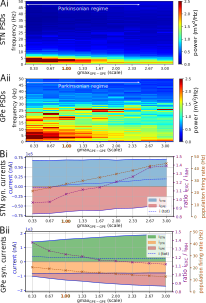
\includegraphics[height=\dimexpr \textheight - 10\baselineskip\relax]{ch_detailed_model/figs_split/fig_endogenous_sweep-gmax-gpe-gpe_A-psd-currents.png}
\caption{
\textbf{Increasing the strength of collateral GPe-GPe inhibition shifts excitation-inhibition balance in STN and GPe in opposite directions.}
Behavior of autonomous STN-GPe network for increasing values of GPe-GPe synaptic conductance. All other parameters were fixed. Default value used in other simulations ({\color{brown} $g_{max}$ scale = 1}) is marked on horizontal axis.
\textbf{A}: Mean PSD of the somatic membrane voltages of STN (Ai) and GPe (Aii) neurons.
\textbf{B}: Balance of excitation and inhibition in the STN (Bi) and GPe (Bii) based on synaptic currents recorded in three neurons. Mean population firing rate (brown), E/I ratio (purple), and net synaptic current (blue). Shaded areas represent estimated total synaptic current from one pre-synaptic population during a simulation.
}
\label{fig:endogenous_sweep-gmax-gpe-gpe_A-psd-currents}
\end{figure}

\begin{figure}
\centering
\includegraphics[width=\textwidth]{ch_detailed_model/figs_split/fig_endogenous_sweep-gmax-gpe-gpe_B-rasters.png}
\caption{
\textbf{Increasing the strength of collateral GPe-GPe inhibition shifts excitation-inhibition balance in STN and GPe in opposite directions.}
Behavior of the autonomous STN-GPe network for increasing values of GPe-GPe synaptic conductance.
\textbf{A-B}: Representative spike trains and phase vectors for STN (green) and GPe population (red) for two values of the GPe to GPe conductance (scale 0.33; 2.0 in A; B respectively). Panels iii shows phase vectors of the STN and GPe populations (in green; red, respectively, mean population vectors plotted as thick solid lines and cell vectors as thin transparent lines) reflecting phase locking to the instantaneous GPe phase.
}
\label{fig:endogenous_sweep-gmax-gpe-gpe_B-rasters-vectors}
\end{figure}

\begin{figure}
\centering
\includegraphics[width=\textwidth]{ch_detailed_model/figs_split/fig_endogenous_sweep-gmax-gpe-gpe_C-metrics.png}
\caption{
\textbf{Phase relationships and aggregate spike metrics in the autonomous STN-GPe network for increasing values of GPe-GPe synaptic conductance.}
\textbf{A}: Population vector length and angle of STN and GPe population (green; red, respectively).
\textbf{B}: Metrics that characterize bursting in STN neurons: median burst rate, intra-burst firing rate, and coefficient of variation of ISIs across all STN cells.
}
\label{fig:endogenous_sweep-gmax-gpe-gpe_C-metrics}
\end{figure}

%
%
%
%
%
%

%
%
\subsection{Strength and time-course of GPe-STN inhibition controls bursting and phase-locking in STN neurons}
%
\label{sec:endogenous_sweep-gpe-stn-gmax-gabaAB}

%
%
%
%
Following dopamine depletion the inhibitory GPe-STN connection is strengthened by a proliferation of synapses and increased decay kinetics of GABA currents \cite{fan_proliferation_2012}. Moreover, the expression of both GABA\textsubscript{A} \cite{fan_proliferation_2012} and GABA\textsubscript{B} \cite{shen_dopamine_2005} receptors is upregulated leading to larger evoked synaptic currents. To investigate the effects of increased inhibition and altered kinetics of inhibitory post-synaptic currents (IPSC) in STN neurons on network activity patterns, an increase in the GABA\textsubscript{A} and GABA\textsubscript{B} conductances was simulated and the relative contribution of both currents was altered.
%
%
%

%
Increasing the conductance of both GABA\textsubscript{A} and GABA\textsubscript{B} synapses lead to an increase in low-frequency bursting of STN neurons (Fig.~\ref{fig:endogenous_sweep-gmax-gpe-stn_A-psd-currents}.A, \ref{fig:endogenous_sweep-gmax-gpe-stn_B-rasters-vectors}.A-B). Bursting was periodic at low frequencies ($\sim$ 2-5 Hz) but was not synchronized between cells (Fig.~\ref{fig:endogenous_sweep-gmax-gpe-stn_B-rasters-vectors}.Bi). Increasing the conductance also shifted the firing mode of STN neurons towards longer bursts with higher intra-burst firing rate against a lower background firing rate, characterized by a high coefficient of variation of ISIs (Fig~\ref{fig:endogenous_sweep-gmax-gpe-stn_A-psd-currents}.B, \ref{fig:endogenous_sweep-gmax-gpe-stn_C-metrics}.B). Bursting with high intra-burst firing rates is mediated by a shift toward net inhibition in STN neurons (Fig~\ref{fig:endogenous_sweep-gmax-gpe-stn_A-psd-currents}.Bi), leading to increased availability of voltage-sensitive $Na^+$ and $Ca^{2+}$ channels through de-inactivation at hyperpolarized membrane voltages \cite{gillies_membrane_2005,baufreton_enhancement_2005,hallworth_globus_2005}. The GPe neuron model does not possess the same high density of $Ca^{2+}$ channels that underlies plateau potentials and strong bursting, and therefore has a lower tendency towards burst firing.
While STN neurons were more weakly entrained to the beta oscillation they preferentially fired in an interval leading the GPe by approximately 65 degrees (Fig~\ref{fig:endogenous_sweep-gmax-gpe-stn_B-rasters-vectors}.Aiii-Biii, \ref{fig:endogenous_sweep-gmax-gpe-stn_C-metrics}.A). The shift toward low-frequency, fast bursting coincided with an increase in synchronization in the network, as measured by the population vector length of the STN and GPe.
%
%
%
%

%
\begin{figure}
\centering
\includegraphics[height=\dimexpr \textheight - 9\baselineskip\relax]{ch_detailed_model/figs_split/fig_endogenous_sweep-gmax-gpe-stn_A-psd-currents.png}
\caption{
\textbf{Increasing the level of GPe-STN inhibition shifts STN to a low-frequency burst firing mode.}
Behavior of autonomous STN-GPe network for increasing values of GPe-STN synaptic conductance. All other parameters were fixed. Default value used in other simulations ({\color{brown} $g_{max}$ scale = 1}) is marked on horizontal axis.
\textbf{A}: Mean PSD of the somatic membrane voltages of STN (Ai) and GPe (Aii) neurons.
\textbf{B}: Balance of excitation and inhibition in the STN (Bi) and GPe (Bii) based on synaptic currents recorded in three neurons. Mean population firing rate (brown), E/I ratio (purple), and net synaptic current (blue). Shaded areas represent estimated total synaptic current from one pre-synaptic population during a simulation.
}
\label{fig:endogenous_sweep-gmax-gpe-stn_A-psd-currents}
\end{figure}

\begin{figure}
\centering
\includegraphics[width=\textwidth]{ch_detailed_model/figs_split/fig_endogenous_sweep-gmax-gpe-stn_B-rasters.png}
\caption{
\textbf{Increasing the level of GPe-STN inhibition shifts STN to a low-frequency burst firing mode.}
Behavior of the autonomous STN-GPe network for increasing values of the GPe to STN synaptic conductance.
\textbf{A-B}: Representative spike trains and phase vectors for STN (green) and GPe population (red) for two values of the GPe to GPe conductance (scale 0.33; 2.0 in A; B respectively). Panels iii shows phase vectors of the STN and GPe populations (in green; red, respectively, mean population vectors plotted as thick solid lines and cell vectors as thin transparent lines) reflecting phase locking to the instantaneous GPe phase.
}
\label{fig:endogenous_sweep-gmax-gpe-stn_B-rasters-vectors}
\end{figure}

\begin{figure}
\centering
\includegraphics[width=\textwidth]{ch_detailed_model/figs_split/fig_endogenous_sweep-gmax-gpe-stn_C-metrics.png}
\caption{
\textbf{Phase relationships and aggregate spike metrics in the autonomous STN-GPe network for increasing values of GPe-STN synaptic conductance.}
\textbf{A}: Population vector length and angle of STN and GPe population (green; red, respectively).
\textbf{B}: Metrics that characterize bursting in STN neurons: median burst rate, intra-burst firing rate, and coefficient of variation of ISIs across all STN cells.
}
\label{fig:endogenous_sweep-gmax-gpe-stn_C-metrics}
\end{figure}

%
%
%
%

%

%

%
To investigate the effect of IPSC kinetics on the generation of beta oscillations within the network, the relative strength of the GABA\textsubscript{A} and GABA\textsubscript{B}-mediated current was changed by decreasing the GABA\textsubscript{B} conductance by 50\% and increasing the GABA\textsubscript{A} conductance progressively (Fig~\ref{fig:endogenous_sweep-gaba-AB-gpe-stn_AC-psd-all}). As this increased the level of inhibition in STN neurons, it resulted in a small shift in the oscillation frequency across the parameter sweep (Fig~\ref{fig:endogenous_sweep-gaba-AB-gpe-stn_AC-psd-all}.A).
%
The simulation results showed that the slow nature of the GABA\textsubscript{B}-mediated current prevented GPe neurons from patterning their targets with short duration IPSC required for strong entrainment in the 20-30 Hz range. When the GABA\textsubscript{A} conductance was increased, and the GABA\textsubscript{B} conductance decreased accordingly, both STN and GPe neurons entrained strongly to the beta rhythm as evident in phase histograms and spike trains (Fig.~\ref{fig:endogenous_sweep-gaba-AB-gpe-stn_B-rasters-phases}). When the experiment of Fig.~\ref{fig:endogenous_sweep-gmax-ctx-stn_A-psd-currents} was repeated in the adjusted network with a higher GABA\textsubscript{A} to GABA\textsubscript{B} ratio, the oscillation frequency in both STN and GPe also showed a clear sensitivity to the strength of the Poisson distributed cortical excitatory input (Fig~\ref{fig:endogenous_sweep-gaba-AB-gpe-stn_AC-psd-all}.B).

%
\begin{figure}
\centering
\includegraphics[height=\dimexpr \textheight - 9\baselineskip\relax]{ch_detailed_model/figs_split/fig_endogenous_sweep-gaba-AB_AC-psd-all.png}
\caption{
\textbf{Endogenous oscillations in the STN-GPe network are strengthened by shifting the GPe-STN synaptic current from slow GABA\textsubscript{B} receptors to fast GABA\textsubscript{A} receptors.}
\textbf{A} Power of population activity in the STN and GPe for increasing values of the GABA\textsubscript{A} to GABA\textsubscript{B} conductance ratio of GPe-STN synapses.
\textbf{B}: Power of population activity in the STN and GPe for increasing CTX-STN conductance and at higher GABA\textsubscript{A}:GABA\textsubscript{B} ratio. The GABA\textsubscript{B} conductance of GPe to STN synapses was halved, and the GABA\textsubscript{A} conductance was doubled.
}
\label{fig:endogenous_sweep-gaba-AB-gpe-stn_AC-psd-all}
\end{figure}

\begin{figure}
\centering
\includegraphics[width=\textwidth]{ch_detailed_model/figs_split/fig_endogenous_sweep-gaba-AB_B-rasters-phases.png}
\caption{
\textbf{Endogenous oscillations in the STN-GPe network are strengthened by shifting the GPe-STN synaptic current from slow GABA\textsubscript{B} receptors to fast GABA\textsubscript{A} receptors.}
\textbf{B-C}: Representative spike trains and phase histograms of STN (green) and GPe neurons (red) in baseline model without scaling of conductances (A-B) and model where GABA\textsubscript{A} conductance was scaled by a factor 6 and GABA\textsubscript{B} conductance was scaled by factor 0.2 (C-D), chosen so that the E/I ratio was close to that in the baseline model (A-B: baseline model, E/I ratio was 0.89; 0.97 in STN, GPe respectively; C-D: scaled conductances, ratio was 0.89; 0.93).
}
\label{fig:endogenous_sweep-gaba-AB-gpe-stn_B-rasters-phases}
\end{figure}

%
%
\subsection{STN-GPe network shows resonant properties and phase locks to cortical beta inputs}
\label{sec:patterned-loop_sweep-burst-freq}

%
The degree of phase locking of the STN-GPe network to synchronous cortical rhythms and its sensitivity to intrinsic network parameters was then examined. The network was simulated with cortical inputs modeled as spike trains exhibiting sparse, synchronous bursts.
%
The frequency of the synchronous cortical inputs was first increased from 3 Hz to 60 Hz and the frequency response and phase locking strength of the STN-GPe loop was estimated (Fig.~\ref{fig:exogenous_ctx-resonance-response_A-power} - \ref{fig:exogenous_ctx-resonance-response_B-vectorlength}). Spectral power and phase locking, measured by the population vector length, were strongest when the cortical oscillation frequency was close to the network's endogenous oscillation frequency (Fig.~\ref{fig:exogenous_ctx-resonance-response_A-power}.C, \ref{fig:exogenous_ctx-resonance-response_B-vectorlength}.A), indicating a resonance effect. Spectral power at the oscillation frequency was increased considerably above that observed for Poisson distributed cortical inputs (compare Fig.~\ref{fig:exogenous_ctx-resonance-response_A-power}.A-AB to Fig.~\ref{fig:endogenous_sweep-gmax-ctx-stn_A-psd-currents}.Ai-Aii). Moreover, the frequencies that were amplified by the STN-GPe network corresponded well to the beta-band, i.e. 13-30 Hz (Fig.~\ref{fig:exogenous_ctx-resonance-response_A-power}.C).
%
%
To study the dependence of the resonance peak on the excitation-inhibition balance in the STN, the cortical input strength was then varied while the oscillation frequency remained fixed (Fig.~\ref{fig:exogenous_ctx-resonance-response_B-vectorlength}.B-C). The range of synaptic conductances was chosen so that the STN population firing rate traversed the experimentally reported range of 17-37 Hz \cite{kita_cortical_2011,mallet_disrupted_2008} in the dopamine depleted state during cortical activation (Fig.~\ref{fig:exogenous_ctx-resonance-example_A-psd-currents}.C).
%
%
Maximum phase locking coincided with frequency of maximum endogenous oscillation power observed in the absence of oscillatory inputs (Fig.~\ref{fig:exogenous_ctx-resonance-response_B-vectorlength}.B-C). The results demonstrate how the resonant frequency of the network can be shifted by changing the excitation-inhibition balance, biasing the network toward a slower or faster oscillation.
GPe neurons synchronized stronger to the oscillatory input compared to STN neurons (Fig.~\ref{fig:exogenous_ctx-resonance-response_A-power}.C, \ref{fig:exogenous_ctx-resonance-response_B-vectorlength}.A, \ref{fig:exogenous_ctx-resonance-example_B-rasters}), which showed a tendency to burst, mirroring the results for spontaneous synchronization in the autonomous STN-GPe network. Analogous to the autonomous loop, when the slow bursting behaviour was reduced by shifting the GPe to STN synaptic current from GABA\textsubscript{B} to faster GABA\textsubscript{A} receptors, synchronization and phase locking of both STN and GPe neurons was greatly increased.
%
%
%
%
%
%
%

%

\begin{figure}
\centering
\includegraphics[width=\textwidth]{ch_detailed_model/figs_split/fig_exogenous_resonance-psd-vectorlength_A-power.png}
\caption{
\textbf{Frequency response of STN-GPe network in response to cortical oscillatory bursting inputs.}
\textbf{A-B}: Power of population activity in the STN (A) and GPe (B) for increasing oscillatory bursting frequency.
\textbf{C}: Mean power of population activity in the STN (green) and GPe (red) neurons, averaged within a 5 Hz wide frequency band centered on the cortical oscillation frequency.
}
\label{fig:exogenous_ctx-resonance-response_A-power}
\end{figure}

\begin{figure}
\centering
\includegraphics[height=\dimexpr \textheight - 10\baselineskip\relax]{ch_detailed_model/figs_split/fig_exogenous_resonance-psd-vectorlength_B-vectorlength.png}
\caption{
\textbf{Phase locking of the STN-GPe network to cortical oscillatory bursting inputs.}
\textbf{A}: Population vector length, indicating strength of phase locking to the cortical oscillation of STN (green) and GPe (red) neurons.
\textbf{B-C}: Change in population vector length (solid lines) for a fixed cortical oscillation frequency (20 Hz, 25 hz, 30 Hz in green, blue, orange, respectively) and increasing CTX-STN input synaptic conductance, reflected in an increased ratio of excitation to inhibition (E/I ratio). Endogenous oscillation power in network without oscillatory cortical input is plotted for comparison (dotted lines, power integrated in 5 Hz band centered on cortical frequency in equivalent simulation with cortical inputs). %
}
\label{fig:exogenous_ctx-resonance-response_B-vectorlength}
\end{figure}

%

\begin{figure}
\centering
\includegraphics[width=\textwidth]{ch_detailed_model/figs_split/fig_exogenous_ctx-resonance-example_A-psd-currents.png}
\caption{
\textbf{Response of STN-GPe network to 20 Hz cortical oscillatory bursting for increasing coupling strength.}
\textbf{A-B}: Power of population activity in STN (A) and GPe (B) as a function of the synaptic conductance of CTX-STN inputs. The peak at 20 Hz reaches a maximum when synapses are at 70\% of their baseline strength, whereas the peak in low-frequency power (2-5 Hz) occurs at 50\%.
\textbf{C}: Balance of excitation and inhibition in the STN based on synaptic currents recorded in three neurons. Population firing rate (brown), E/I ratio (purple), and net synaptic current (blue).
}
\label{fig:exogenous_ctx-resonance-example_A-psd-currents}
\end{figure}

\begin{figure}
\centering
\includegraphics[width=\textwidth]{ch_detailed_model/figs_split/fig_exogenous_ctx-resonance-example_B-rasters.png}
\caption{
\textbf{Spiking patterns in response to 20 Hz oscillatory bursting in cortical neurons.}
\textbf{A}: Cortical oscillatory bursting pattern illustrated using representative spike trains. In each cycle of the oscillation 10\% of cells were selected at random to fire a burst in phase with the oscillation, with a variation of 1 ms on the onset and spike timings.
\textbf{B}: Representative spike trains of STN (A) and GPe neurons (B) in simulation with synaptic conductances scaled to 70\%, corresponding to maximum phase locking and 20 Hz power.
}
\label{fig:exogenous_ctx-resonance-example_B-rasters}
\end{figure}

%
%
\subsection{Influence of phase relationship between cortical and striatal beta inputs}
\label{sec:patterned-loop_sweep-ctx-msn-phase}
%
%
%
%
%
%
%
%
%

%
Striatal microcircuits exhibit beta-band oscillations in healthy primates \cite{feingold_bursts_2015} and parkinsonian rodent models \cite{mccarthy_striatal_2011,sharott_population_2017} and have been hypothesized to be part of the pacemaking circuit that generates them. In the previous section, the STN-GPe network was shown to generate weak beta-band oscillations in the absence of exogenous beta inputs  (Fig.~\ref{fig:endogenous_sweep-gmax-ctx-stn_A-psd-currents},~\ref{fig:endogenous_sweep-gmax-gpe-gpe_A-psd-currents},~\ref{fig:endogenous_sweep-gmax-gpe-stn_A-psd-currents}), and to phase lock to cortical beta-band inputs which amplified oscillatory activity (Fig.~\ref{fig:exogenous_ctx-resonance-response_A-power} - \ref{fig:exogenous_ctx-resonance-response_B-vectorlength}). A potential role of the pallido-striatal loop could be to amplify beta-band oscillations in the STN-GPe network to a more pathological level, as part of a double resonant loop converging on the GPe. A suggested mechanism is that altered striatal activity in PD could shift the phase of firing of the GPe relative to the STN to one that supports STN phase locking through increasing the availability of $Na^{+}$ and $Ca^{2+}$ channels post-inhibition and pre-excitation \cite{baufreton_enhancement_2005,mallet_parkinsonian_2008,mallet_dichotomous_2012}. Alternatively, oscillations that originate in striatal circuits could be transmitted via the striato-pallidal projection and thus introduced into the STN-GPe network \cite{mccarthy_striatal_2011,corbit_pallidostriatal_2016}. Of the two loops converging on GPe neurons, inhibitory striatal afferents would be better suited to interrupt ongoing activity and influence the phase compared to excitatory STN afferents. Hence, the iMSN to GPe projection could play an important role in patterning neural activity in the STN-GPe network.
%

Phase vector plots in the previous section show that STN and GPe neurons settle into a particular phase relationship where STN leads GPe by 60-90 degrees which contributed to sustaining beta-band oscillations. It was hypothesized that inhibitory inputs from the striatum would either disrupt this phase relationship, thereby suppressing beta-band oscillations, or reinforce them depending on where in the phase of the beta oscillation they arrive. To investigate this hypothesis, surrogate striatal spike trains exhibiting beta frequency bursts were generated and the phase with respect to the incoming cortical oscillation was increased in increments of 45 degrees by varying the onset time of bursts. As iMSN-GPe synapses exhibit short-term facilitation, bursts administered through this projection led to an increase in inhibition to the GPe that was greater than the relative increase in spike rate. To compensate for this effect and maintain a physiological firing rate range of the GPe neurons, the peak conductance of iMSN-GPe synapses was reduced by 60\%.

%
Varying the phase of striatal relative to cortical bursts revealed that populations connected by an inhibitory projection, i.e. iMSN, GPe, and STN maintained a rigid phase relationship with respect to the cortical oscillation (Fig.~\ref{fig:exogenous_sweep-ctx-msn-phase_B-rasters}: population vectors in green, red, purple formed a rigid frame that rotated relative to the cyan-colored cortical population vector). The local maximum in phase locking occurred when excitatory CTX and inhibitory GPe afferents to STN fired in anti-phase, occurring when the CTX-iMSN phase difference was set to 225 degrees (Fig.~\ref{fig:exogenous_sweep-ctx-msn-phase_A-psd-currents}.B, \ref{fig:exogenous_sweep-ctx-msn-phase_B-rasters}.B, \ref{fig:exogenous_sweep-ctx-msn-phase_C-metrics}.B). This supports the feedback inhibition hypothesis where cortical patterning is promoted when GPe-STN inhibition is offset in phase relative to cortical excitation in PD \cite{baufreton_enhancement_2005,mallet_parkinsonian_2008,mallet_dichotomous_2012}. The changing phase relationship of cortical spiking relative to the three other populations also shifted the balance of excitatory and inhibitory currents in the STN (Fig.~\ref{fig:exogenous_sweep-ctx-msn-phase_A-psd-currents}.Bi). Maximum phase locking occurred where the STN was maximally inhibited (E/I ratio $\approx$ 1.1, population firing rate $\approx$ 21 Hz), whereas minimum phase locking coincided with maximum excitation (E/I ratio $\approx$ 1.3, population firing rate $\approx$ 40 Hz). In the GPe this relationship between phase locking strength and firing rate was reversed (Fig.~\ref{fig:exogenous_sweep-ctx-msn-phase_A-psd-currents}.Bii) whereas the relationship with E/I ratio showed no clear trend. The optimal phase relationship of 225 degrees further strengthened phase locking to the applied beta rhythm compared to the situation with only cortical oscillatory inputs. Maximum vector length was increased by a factor of two, confirming increased synchronization, in both populations when compared to the case where only cortical beta frequency inputs were simulated. Maximum power at the oscillation frequency was also increased by a factor of approximately 2.7 in STN and 5.2 in GPe.
%
%
%
%
%
%
%
%
%
%
%
%
%
%
%


%

\begin{figure}
\centering
\includegraphics[height=\dimexpr \textheight - 10\baselineskip\relax]{ch_detailed_model/figs_split/fig_exogenous_sweep-ctx-msn-phase_A-psd-currents.png}
\caption{
\textbf{The phase relationship between cortical and striatal beta-band inputs to the STN-GPe network affects the strength of phase-locking by setting the relative timing of excitatory and inhibitory STN afferents.}
\textbf{A}: Power of population activity in STN (Ai) and GPe (Aii), showing weakening and strengthening of oscillations as relative phases of inputs are rotated.
\textbf{B}: Balance of excitation and inhibition in the STN (Bi) and GPe (Bii) based on synaptic currents recorded in three neurons. Population firing rate (brown), E/I ratio (purple), and net synaptic current (blue). Shaded areas represent estimated total synaptic current from one pre-synaptic population during a simulation.
}
\label{fig:exogenous_sweep-ctx-msn-phase_A-psd-currents}
\end{figure}

\begin{figure}
\centering
\includegraphics[width=\textwidth]{ch_detailed_model/figs_split/fig_exogenous_sweep-ctx-msn-phase_B-rasters.png}
\caption{
\textbf{The phase relationship between cortical and striatal beta-band inputs to the STN-GPe network affects the strength of phase-locking by setting the relative timing of excitatory and inhibitory STN afferents.}
Representative spike trains and phase vectors of STN (green) and GPe population (red) for CTX-iMSN phase difference of $90^\circ$ (A) and $225^\circ$ (B). Panels iii shows phase vectors of the STN, GPe, CTX, iMSN populations (in green; red; blue; purple, respectively; mean population vectors plotted as thick solid lines and cell vectors as thin transparent lines).
}
\label{fig:exogenous_sweep-ctx-msn-phase_B-rasters}
\end{figure}

\begin{figure}
\centering
\includegraphics[width=\textwidth]{ch_detailed_model/figs_split/fig_exogenous_sweep-ctx-msn-phase_C-metrics.png}
\caption{
\textbf{The phase relationship between cortical and striatal beta-band inputs to the STN-GPe network affects bursting tendency and temporal spike dispersion in the STN.}
\textbf{A}: Population vector length and angle of STN (green) and GPe (red) population.
\textbf{B}: Metrics that characterize bursting in STN neurons: median burst rate, intra-burst firing rate, and coefficient of variation of ISIs across all STN cells.
}
\label{fig:exogenous_sweep-ctx-msn-phase_C-metrics}
\end{figure}

%
%
\subsection{Mechanism of phase locking}

%
%
%
%

%
%
%

To further illustrate the interaction between synaptically coupled STN and GPe neurons in the model under conditions of synchronous oscillatory beta-band activity, the mechanism of phase locking of STN cells is presented in Fig.~\ref{fig:cell-phaselocking-mechanisms}. Pooled cortical spike trains (Fig.~\ref{fig:cell-phaselocking-mechanisms}.A-B, green) illustrate how sparse cortical beta bursts (Fig.~\ref{fig:exogenous_ctx-resonance-example_B-rasters}.A) result in distributed synaptic inputs to individual STN neurons that are not tightly phase locked, but have a combined firing rate that is modulated at the beta frequency. While these exogenous cortical inputs had high spike timing variability, STN and GPe spikes became highly structured and tightly locked to the beta oscillation through the feedback inhibition mechanism. The cortical beta modulation is transmitted to the STN and then to the GPe through their excitatory projections (see phase vectors in Fig.~\ref{fig:exogenous_sweep-ctx-msn-phase_B-rasters}). When the inhibitory feedback arrives back in STN this shuts down spiking (Fig.~\ref{fig:cell-phaselocking-mechanisms}.A) and simultaneously primes the cell for the next period of increased cortical excitation by de-inactivating $Ca^{2+}$ channels (Fig.~\ref{fig:cell-phaselocking-mechanisms}.C) and $Na^{+}$ channels. As the cortical firing rate rises again, synaptic currents (Fig.~\ref{fig:cell-phaselocking-mechanisms}.B) combine with dendritic $Ca^{2+}$ currents to overcome any lingering inhibition and cause the next wave of phase-locked STN spikes. The striatal beta inputs further decreased spiking variability of GPe neurons by narrowing their time window of firing through phasic inhibition (purple phase vector in Fig.~\ref{fig:exogenous_sweep-ctx-msn-phase_B-rasters}).

%

%
\begin{figure}
\centering
\includegraphics[height=\dimexpr \textheight - 15\baselineskip\relax]{ch_detailed_model/figs/fig_cell-phaselocking-mechanisms.png}
\caption{\textbf{Mechanisms contributing to phase locking of STN cells to cortical beta oscillations.} Recordings of synaptic currents and T-type calcium (CaT) channel inactivation from an identified phase-locked STN cell during a simulation with high phase locking. Inactivation variables were recorded from each compartment with CaT ion channels and averaged over all compartments in the cell. Zero-crossings of the instantaneous beta phase are indicated using vertical dotted lines. \textbf{A}: Somatic membrane voltage during phase-locked interval (blue). Spike trains from excitatory (green) and inhibitory (red) afferents to the cell were pooled. \textbf{B}: Total excitatory and inhibitory synaptic current (in green; red, respectively) and pooled spike trains underneath. \textbf{C}: Mean CaT channel inactivation across the cell's dendritic tree. High values correspond to de-inactivation. Transient de-inactivation approximately one half period after an inhibitory barrage engages depolarizing T-type $Ca^{2+}$ current and contributes to phase-locked spiking.}
\label{fig:cell-phaselocking-mechanisms}
\end{figure}

%
%
%

%

%
%
%
%
%
%
%
%
%
%
%

%
%
%
\section{Discussion}
\label{sec:ch3-discussion}
%
%
%
%
%
%
%
%
%
%

%
%
A new model of the STN-GPe network is presented that incorporates biophysically detailed multi-compartment cell models. The individual STN and GPe cell models capture the interaction of intrinsic and synaptic membrane currents with nonuniform subcellular distributions across the dendritic structure, which can not be captured in single compartment models. The model illustrates how phase locking of STN and GPe neurons, and increased bursting of STN neurons, can arise from the interaction of these currents when their relative strengths and temporal relationships are altered. The STN-GPe model network showed an intrinsic susceptibility to beta-band synchrony that manifest as weak, autonomously-generated endogenous oscillations and selective amplification of exogenous beta-band synaptic inputs at the network's preferred oscillation frequency.  The frequency at which endogenous beta oscillatory activity occurred varied with the ratio of excitatory to inhibitory currents to the STN. Varying the phase relationships between external beta-frequency inputs to the network through cortical and striatal pathways further increased or suppressed the level of amplification of cortical beta inputs by modulating the temporal dispersion of action potentials in STN neurons and thereby influencing the precision of phase locking.
%
Varying synaptic strengths within the network affected the balance of excitation and inhibition in both STN and GPe neurons and produced a rich set of behaviors, not only modulating firing rates but also affecting synchronization and bursting properties of neurons. Homeostatic mechanisms mediated by feedback connections and short-term synaptic plasticity dynamics served to stabilize the excitation-inhibition balance in the GPe and reduced the sensitivity of its population firing rate to variations in pre-synaptic rates.

%
\subsection{Oscillatory properties of the multi-compartmental STN-GPe network}
%
In the autonomous STN-GPe network, under conditions of Poisson distributed external synaptic inputs, STN neurons exhibited weak synchronization to the endogenous beta rhythm but retained a weak phase preference with respect to the stronger oscillation in the GPe population (Fig.~\ref{fig:endogenous_sweep-gmax-ctx-stn_B-rasters-vectors} - ~\ref{fig:endogenous_sweep-gmax-gpe-stn_B-rasters-vectors}). The synchronization strength of STN neurons was found to depend on the relative strength of GABA\textsubscript{A} and GABA\textsubscript{B} receptors in STN dendrites (Fig.~\ref{fig:endogenous_sweep-gaba-AB-gpe-stn_AC-psd-all}, \ref{fig:endogenous_sweep-gaba-AB-gpe-stn_B-rasters-phases}), with an increase in the proportion of fast-acting GABA\textsubscript{A} receptors resulting in an increase in the strength of oscillation. The endogenous oscillation frequency of the STN-GPe network was further influenced by the balance of excitatory and inhibitory currents in the STN. This balance affected the net level of excitatory drive in the network, shifting the oscillation frequency towards the higher beta range for increased levels of excitatory drive (Fig.~\ref{fig:endogenous_sweep-gmax-ctx-stn_A-psd-currents}.A, \ref{fig:endogenous_sweep-gaba-AB-gpe-stn_AC-psd-all}.B).
Besides affecting population firing rates and the frequency of synchronous oscillations, the excitation-inhibition balance also strongly influenced the firing pattern of STN neurons: for a low ratio of excitation to inhibition and sufficiently strong inhibitory currents, STN neurons transitioned to a firing mode characterized by low-frequency tight bursts (high intra-burst firing rate, Fig.~\ref{fig:endogenous_sweep-gmax-ctx-stn_A-psd-currents}-~\ref{fig:endogenous_sweep-gmax-gpe-stn_C-metrics}). Low-frequency bursting was periodic at 2-5 Hz but was not synchronized between cells. This shift in firing pattern towards sparse, tight bursting is in correspondence with changes in burst-related measures such as intra-burst firing rate and sub-beta band power that are most predictive of akinetic-bradykinetic symptoms in humans \cite{sharott_activity_2014} and monkeys \cite{sanders_parkinsonism-related_2013}. The firing rate and pattern of GPe neurons was less sensitive than that of STN neurons to variations in its excitatory or inhibitory drive due to the contribution of negative feedback control by homeostatic mechanisms that operated in synergy to stabilize its E/I ratio. However, GPe neurons did synchronize more strongly under conditions of low excitatory drive from the STN enabling them to act more autonomously and synchronize through inhibitory collaterals within the GPe network.
%
%

%
%
%
%
%
When beta-band spiking inputs were applied to the STN-GPe network via cortico-STN afferents, the STN-GPe network phase locked to the beta rhythm. Frequencies near the autonomous oscillation frequency for a given E/I ratio were preferentially amplified, reflected in increased phase locking and power of the somatic membrane voltage at that frequency (Fig.~\ref{fig:exogenous_ctx-resonance-response_A-power} - \ref{fig:exogenous_ctx-resonance-response_B-vectorlength}). This is supportive of experimental observations that oscillatory activity in STN is contingent on cortical oscillations \cite{magill_dopamine_2001}, likely transmitted though the hyperdirect pathway \cite{tachibana_subthalamo-pallidal_2011}. Phase locking and beta frequency power were further strengthened by the addition of striatal oscillatory inputs with a particular phase relationship to cortical oscillatory inputs (Fig.~\ref{fig:exogenous_sweep-ctx-msn-phase_A-psd-currents} - \ref{fig:exogenous_sweep-ctx-msn-phase_B-rasters}).
Maximum phase-locking occurred when GPe spiking was aligned in anti-phase with cortical inputs to the STN (Fig.~\ref{fig:exogenous_sweep-ctx-msn-phase_B-rasters}.B, \ref{fig:exogenous_sweep-ctx-msn-phase_C-metrics}.A). When excitation and inhibition occurred in anti-phase, inhibition was likely more effective at transiently hyperpolarizing the membranes of STN neurons, suggested by the local minimum in their E/I ratio (Fig.~\ref{fig:exogenous_sweep-ctx-msn-phase_A-psd-currents}.Bi). Strong hyperpolarization can evoke low-latency, temporally precise responses to an excitatory stimulus by de-inactivating $Ca^{2+}$ and $Na^{+}$ channels, and thereby priming them to respond to excitatory cortical inputs \cite{bevan_gabaergic_2007}. This mechanism may be responsible for the increase in phase locking under this phase relationship.
In contrast, phase alignment of cortical and GPe neurons, corresponding to coincident firing, desynchronized STN neurons (Fig.~\ref{fig:exogenous_sweep-ctx-msn-phase_B-rasters}.A). These findings are in agreement with recent experimental observations which demonstrate that co-stimulation of GABAergic and glutamergic STN afferents disperses STN spiking and has a desynchronizing effect on the population \cite{steiner_connectivity_2019}.

Overall, the simulation results are consistent with the hypothesis of cortical patterning and resonance of beta activity within the STN-GPe network through feedback inhibition, whereby GPe inhibition arriving in anti-phase to cortical excitation promotes phase locking of STN neurons to beta-band cortical inputs \cite{baufreton_enhancement_2005}. The model predicts that exaggerated phase locking of the STN-GPe
loop to external oscillatory inputs arises in Parkinsonian conditions as a result of a new balance of excitatory to inhibitory inputs to the STN and GPe.
Moreover, it predicts that this exaggerated phase locking is not only contingent on cortical
oscillations arriving through the hyperdirect pathway, but that striatal oscillations arriving
through the indirect pathway are also crucial in setting an anti-phase relationship
between cortex and GPe activity that maximizes cortical patterning of the STN.
%

%
%
%
%

\subsection{Relation of mechanism of oscillations to other models of oscillatory activity in the STN-GPe network}
\label{sec:ch3-disc:osc-mech-others}

%
%
%

%
The mechanism by which oscillatory neural activity can be generated in the STN-GPe network, by alternating phases of excitation and inhibition in a delayed negative feedback loop, has been described in previous models \cite{terman_activity_2002,holgado_conditions_2010,kumar_role_2011}. The mechanism of oscillation in the model presented here is consistent with this, and the model additionally illustrates the dual role of precisely timed GPe inhibition in transiently reducing STN neuron excitability and hyperpolarising them such that they are primed to respond with bursting to excitatory cortical inputs (Fig.~\ref{fig:cell-phaselocking-mechanisms}). Furthermore, it highlights the sensitivity of the network oscillation to the excitation-inhibition balance in each population and synaptic current properties.

%
In the multicompartment model, endogenously generated beta frequency oscillations were generated within the STN-GPe network when the strength of short duration GABA\textsubscript{A}-mediated currents was increased. Since the slow timescale, signaling cascade-mediated GABA\textsubscript{B} currents are typically not modeled, this result can be easily reconciled with results from single-compartment and firing rate models where high gain within the closed-loop is a necessary condition for strong endogenously-generated oscillations in the STN-GPe network \cite{holgado_conditions_2010,pavlides_improved_2012,park_neural_2011,wei_role_2015}. The strength of the endogenous oscillations in the current model was relatively weak, except when inhibitory GPe-STN currents were strongly dominated by fast-acting GABA\textsubscript{A}-mediated currents and GABA\textsubscript{B}-mediated slow currents were weak. The oscillation frequency of the network could be modulated by varying the ratio of excitation to inhibition in STN and GPe, and increased as this ratio increased (Fig.~\ref{fig:exogenous_ctx-resonance-response_B-vectorlength}) .

%
The oscillation frequency of the network has been shown to be sensitive to model parameters in previous computational models of the BGTC network. Specifically, in mean field models of the STN-GPe loop the oscillation frequency showed a strong sensitivity to transmission delays and neuronal membrane time constants \cite{holgado_conditions_2010,lienard_beta-band_2017}, and a weaker sensitivity to coupling strengths \cite{holgado_conditions_2010,pavlides_computational_2015,liu_neural_2017}, also demonstrated in a spiking model \cite{wei_role_2015}. In the multicompartment model presented here, where active ion channels on the dendrites contribute to synaptic integration, synaptic strength and effective membrane time constant are interdependent since the membrane charging speed is affected by transient activation of ion channels as a response to synaptic inputs. In biological neurons the balance of excitation and inhibition is tightly regulated through multiple adaptive processes \cite{turrigiano_too_2011}, and likely maintains the range of possible oscillation frequencies within a narrow range.

%
%
%

%
Other than the condition where GPe-STN currents were dominated by fast-acting GABA\textsubscript{A} currents, strongly synchronized beta-band oscillations appeared only when exogenous beta-band inputs were introduced to the network (Fig.~\ref{fig:exogenous_ctx-resonance-response_A-power}, \ref{fig:exogenous_sweep-ctx-msn-phase_A-psd-currents}, \ref{fig:exogenous_sweep-ctx-msn-phase_B-rasters}). These results, therefore, support a role for resonance with oscillations throughout other basal ganglia loops in the generation of increased STN-GPe beta activity in Parkinson's disease. Such an oscillatory drive can be provided either by an extrinsic oscillator, assumed to originate within the cortex in the present model, or by reverberation of oscillations in connected feedback loops such as the pallido-striatal loop \cite{corbit_pallidostriatal_2016}, intra-striatal loops \cite{mccarthy_striatal_2011}, or the larger thalamocortical loop \cite{pavlides_computational_2015,kang_interaction_2013,reis_thalamocortical_2019,dovzhenok_origin_2012}.
%
The model exhibited clear resonance in response to excitatory synaptic inputs to the STN within the beta frequency range (Fig.~\ref{fig:exogenous_ctx-resonance-response_A-power} - \ref{fig:exogenous_ctx-resonance-response_B-vectorlength}). The frequency at which the maximum resonance occurred increased with increasing ratio of excitation to inhibition, similar to the increase in frequency observed in the case of endogenously generated oscillations. Resonance phenomena in the beta-band have previously been reported in computational models of basal ganglia networks, consistent with the modeling results presented here: \cite{pavlides_computational_2015} fitted mean field rate models to experimental data from nonhuman primates and found that the models that best explained the data relied on a strong cortical oscillation to sustain beta-band oscillations ($\sim 15$ Hz) in the network. \cite{ahn_synchronized_2016} using 10 single compartment STN and GPe neurons observed multiple resonances in the beta-band when varying the strength of striato-pallidal and pallida-subthalamic inhibition, with resonant peaks occurring consistently between 18-21 Hz. Similarly, \cite{fountas_role_2017} found that STN neurons in their model exhibited high spontaneous beta-band power (18-30 Hz) and synchronized selectively with cortical input in this frequency range.

%
%
%
%

%
%

%
%

%
%
%

%
%
%

%
%
%
%
%
%

%
\subsection{Model complexity and limitations}
\label{sec:ch3-limitations}

%
%
%
%
%
One of the main advantages of the biophysically detailed model presented here is that the model can capture the nonuniform distribution of afferent inputs from different pre-synaptic populations across the dendritic tree (Table~\ref{tab:stn_synaptic_currents},~\ref{tab:gpe_synaptic_currents}). This targeting of specific regions of the dendrites by different populations can lead to variations in synaptic integration properties within the structure. This feature is potentially of particular importance in the generation of pathological oscillations given that neuronal phase response curves, used to quantify the tendency of neurons to synchronize to their inputs, differ when stimuli are applied to different subcellular regions in STN and GPe neurons \cite{schultheiss_phase_2010,farries_phase_2012}. Hence, a model that incorporates a full complement of ion channel and the synapse groups that interact with them may be expected to yield a more realistic representation of how synchronization arises in the network. In future studies, this could also contribute to a better understanding of neuronal currents contributing to the local field potential in synchronized and asynchronous states, as synaptic and ionic transmembrane currents combine to form the extracellular currents that underpin this signal \cite{buzsaki_origin_2012}.
%

%
%
A second advantage of such detailed multicompartment models is that parameters have a clear relationship to the underlying biophysical system and are more meaningful in terms of physiological processes compared to models where parameters are lumped, as in single-compartment conductance-based models, or abstracted as in mean-field or generalized integrate-and-fire models. This allows for a more direct translation of experimental findings to parameter variations in the model. On the other hand, detailed cell models are more sensitive to correct estimation of these parameters which is limited by measurements performed for the purpose of model fitting as well as the fitting procedures themselves.

%
%
Biophysically detailed models offer new ways to study factors contributing to the development of synchrony. Such models provide a means to investigate the relative contributions of physiological mechanisms to the development of synchrony while controlling other factors in a manner that is not possible in vivo. Though the model presented incorporates a higher level of physiological detail than previous models of the STN-GPe network, several simplifications were  necessary due to the model complexity, which should be considered.

\subsubsection*{Biological realism and variability}
%

To model the effects of dopamine depletion on neuron physiology,
downregulation of HCN channel currents with dopamine depletion was modeled as a decrease in its peak conductance. However, dopamine is known to interact with several more ion channels that are involved in linearizing the current-firing rate curve and regularizing autonomous pacemaking of STN neurons \cite{ramanathan_d2-like_2008,yang_d2_2016,loucif_depolarisation_2008}. These channels are not included in the STN cell model used here \cite{gillies_membrane_2005}. Recent evidence suggests that the loss of autonomous spiking is a necessary condition for the exaggerated cortical patterning of STN related to motor dysfunction \cite{mciver_chemogenetic_2018}. Better characterization of the ion channels involved in pacemaking and their response to dopamine depletion will enable the systematic exploration of their contribution to STN response properties and pathological firing patterns.

Furthermore, variability in morphological, electrical, and biophysical properties of neurons within
populations was not fully captured.
%
In the GPe, two distinct populations have been identified based on their molecular profile and axonal connectivity \cite{mallet_dichotomous_2012}. Only the prototypic sub-population projecting mainly to STN and preferentially firing in anti-phase to it was modelled here, with the arkypallidal sub-populations projecting back to striatum omitted. Moreover, the GPe cell model used was only one representative candidate out of a large set of models with varying ion channel expression and morphology that matched a corresponding database of electrophysiological recordings \cite{gunay_channel_2008}.
%
Similarly, the STN model represents a stereotypic characterization rather than a reconstruction of a specific STN cell and does not capture variability in firing properties and receptor expression. In particular, STN neurons in vivo are known to have variable expression of GABA\textsubscript{B} receptors \cite{galvan_differential_2004} which cause strong hyperpolarization responses and longer pauses in some but not all STN neurons \cite{hallworth_globus_2005} and a strong rebound burst response \cite{galvan_differential_2004} in a subset of these. A model that accounts for the biological variability in GABA\textsubscript{B} expression and that of channels underlying the rebound response may reveal a wider range of responses to increased inhibition among STN neurons. In such a model, beta rhythms could be transmitted to a subset of STN neurons whereas others would show longer pauses with stronger rebound bursts. Moreover, the GABA\textsubscript{B} synapse model used does not fully account for activation of extrasynaptic GABA\textsubscript{B}R due to GABA spillover \cite{galvan_differential_2004} which is mediated by tonic high-frequency \textit{and} coincident firing of afferents \cite{bevan_cellular_2006}. A model where multiple GABAergic synapses act on a shared pool of extrasynaptic GABA\textsubscript{B}R might increase the importance of synchronized pre-synaptic activity in switching STN neurons to a burst-firing mode.
%
%

\subsubsection*{Neuronal firing patterns and their analysis}

%
The main sources of firing rate variability in the model were randomness in the input spiking patterns, the presence of surrogate Poisson spike sources in STN and GPe, membrane noise, and randomness in connection patterns and the position of synapses. However, as discussed above, these factors do not capture firing pattern variations arising from variability in morpho-electric cell types between and within sub-populations, and from sub-population specific projection patterns.

%
The effect of the correlation between cortical and striatal inputs to the network was explored by varying the relative phases of both populations when firing in a synchronous oscillatory pattern (Fig.~\ref{fig:exogenous_sweep-ctx-msn-phase_A-psd-currents} - \ref{fig:exogenous_sweep-ctx-msn-phase_B-rasters}). Uncorrelated firing between both populations was also explored (Fig.~\ref{fig:endogenous_sweep-gmax-ctx-stn_A-psd-currents}-\ref{fig:exogenous_ctx-resonance-example_B-rasters}). In reality, beta activity in both populations is likely to be correlated as the striatum receives topographic inputs from the same cortical areas projecting to the STN. Such correlation could lead to transient synchronization effects not explored here, that could promote or counteract additional oscillatory synchronization depending on the exact phase relationships.
%
%
%
%
%
The effect of varying connectivity patterns between neuronal populations was not directly explored here. The development of neural synchronization and oscillatory activty are known to be dependent on network topology \cite{zhao_synchronization_2011}, and this effect has previously been studied in a single compartment model of the STN-GPe network \cite{terman_activity_2002}. The network topology used in the present study is closest to the random, sparsely-connected topology in Terman et al., (2002) which was shown to develop synchronized bursting patterns at lower frequencies. Choosing different randomly-generated connection matrices did not qualitatively change the results, however altering the connection topology would likely lead to different synchronization properties. Moreover, it is known that connection patterns within the basal ganglia are altered with dopamine depletion, particularly within the striatum \cite{cho_dopamine_2002}, leading to a loss of input specificity in neuronal responses \cite{bronfeld_loss_2011}. These alterations in connection patterns and resulting effects on spike correlations were not taken into account as cortico-striatal connectivity was not considered in the model. As arkypallidal GPe neurons were not modelled, the pallido-striatal feedback loop was not captured. This additional feedback loop has also been suggested as a candidate pacemaker circuit for beta-band oscillations \cite{corbit_pallidostriatal_2016}, however, blocking of striatal inputs was not found to reduce the power of beta oscillations in rat GPe \cite{tachibana_subthalamo-pallidal_2011}.
%


%
%
%
%
%
%
%
%
%
Phase synchronization between spike trains was measured by calculating the vector length
of spike trains in the STN and GPe populations based on a band-pass filtered and Hilbert-transformed
reference signal \cite{lachaux_measuring_1999}. This is a frequency-specific measure of
phase synchronization and it was used here to measure spike synchronization in the beta band
within populations. A measure of phase synchronization assumes that the signals are also
oscillatory in nature, in contrast to alternative, more general measures of spike train
synchronization. Because GPe neurons showed a stronger oscillatory characteristic and
power in the beta band (see power spectral densities in Fig.~\ref{fig:endogenous_sweep-gmax-gpe-gpe_A-psd-currents},\ref{fig:endogenous_sweep-gaba-AB-gpe-stn_AC-psd-all},\ref{fig:exogenous_ctx-resonance-response_A-power},\ref{fig:exogenous_ctx-resonance-example_A-psd-currents}) this resulted in higher measures of phase synchronization in the GPe population
compared to the STN. Were synchronization analysis to be performed over a broader
frequency band, or without assuming oscillatory signals, different synchronization
characteristics may be observed. For example, a frequency-dependent measure of
synchronization could be obtained using the composite spike train coherence \cite{terry_how_2008},
applied in a combinatorial fashion \cite{mcmanus_muscle_2016}.
%
%
%
%

%
%
Burst detection was performed using a simple threshold on the ISIs and did not take
into account variations in the background firing rate in the criterion for distinguishing
bursts from background firing. Because of this, the detected burst rates in Fig.~\ref{fig:endogenous_sweep-gmax-gpe-stn_C-metrics},\ref{fig:endogenous_sweep-gmax-gpe-gpe_C-metrics},
\ref{fig:exogenous_sweep-ctx-msn-phase_C-metrics} are strongly correlated with the
mean population firing rates. Alternative burst detection algorithm exist that do take this
into account. For instance, burst detection based on the Poisson surprise method \cite{legendy_bursts_1985}
distinguishes bursts based on the probability of observing a given sequence of spikes
in a random Poisson spike train. Such a burst detection algorithm would decrease the number of
bursts observed at high background firing rates and would lead to a detection rate
more strongly correlated with the CV measurements in Fig.~\ref{fig:endogenous_sweep-gmax-gpe-stn_C-metrics},
\ref{fig:endogenous_sweep-gmax-gpe-gpe_C-metrics},\ref{fig:exogenous_sweep-ctx-msn-phase_C-metrics}.

\subsubsection*{Model fitting}

%
%
%
%
%
%
%
%
%

%
%
%
%
%
%
%

%
%
%
%
%
%
%
%

The parameters representing biophysical quantities in the network model were based on
experimentally reported values found in the literature where available (Section~\ref{sec:ch3-methods}). Synaptic strengths were hand-tuned to obtain population firing rates falling within experimentally
reported ranges, and are therefore fitted in an \textit{ad hoc} manner rather than using a formalized
optimization procedure and cost function. Besides the considerable computational resources
required to perform numerical optimization with a large and detailed network model, a lack of
publicly available electrophysiology data made the use of numerical optimization unsuitable
for the purpose of this study.
In previously published network models of the basal ganglia, optimization is most commonly performed
at the level of neuron models, and the strength of synaptic inputs and bias currents
are then hand-tuned (e.g. \cite{terman_activity_2002,kumar_role_2011,corbit_pallidostriatal_2016,lindahl_untangling_2016,fountas_role_2017}).
The same approach was followed here, given that the neuron models used were optimized using
multi-objective optimization approaches based on patch-clamp recordings \cite{gillies_membrane_2005,gunay_channel_2008}.
Models consisting of single-compartment neurons are more amenable to numerical
optimization due to their lower computational complexity (e.g. \cite{hahn_modeling_2010}),
however the sparsity of data available to constrain optimizations compared to the number
of parameters in the model, makes such optimization prone to overfitting.
While the same can be said for hand-tuning based on data about mean population firing rates,
two observations suggest that at least the behavior of the current model is not the
result of an unstable local minimum in its parameter space. First, as indicated by the
parameter sweeps of synaptic conductances (Fig.~\ref{fig:endogenous_sweep-gmax-ctx-stn_A-psd-currents}-
\ref{fig:endogenous_sweep-gmax-gpe-stn_B-rasters-vectors}), there is a gradual transition
in the network behavior, in terms of its firing rates and oscillation frequencies.
Second, it was verified that altering the randomly-generated connection matrices
while conserving the numbers of inputs to each cell did not strongly affect
the observed firing rates, nor the oscillation or bursting patterns exhibited by the network.
However, the network behavior may still be highly sensitive to other parameters,
e.g. the biophysical parameters of the neuron models used.

\subsubsection*{Relevance of beta-band oscillations}

%
Finally, while there is consistent evidence of increased beta-band oscillatory activity in Parkinson’s disease \cite{sharott_dopamine_2005,mallet_disrupted_2008} and a reduction of pathological beta-band activity with interventions that improve symptoms in patients and animal models of the disease \cite{kuhn_reduction_2006,weinberger_beta_2006,eusebio_deep_2011,ray_local_2008}, strong evidence in support of a causal role for pathological beta activity in the symptoms of Parkinson’s disease has yet to be established. Indeed, recent studies failed to find evidence of any causal link between artificially induced beta-band activity and motor impairment in parkinsonian rats \cite{swan_beta_2019}, nor between the reduction of beta-band activity and alleviation of motor symptoms \cite{pan_neuronal_2016}. A lack of causality, however, may not necessarily be incompatible with the use of beta-band oscillations as a clinical biomarker, particularly for akinetic-bradykinetic forms of Parkinson's disease at advanced stages of disease progression. Initial trials of adaptive or closed-loop deep brain stimulation strategies targeted at suppression of beta-band activity have been successful in demonstrating simultaneous reductions in patient symptoms \cite{little_adaptive_2013,velisar_dual_2019}.  Beta-band power may thus still be a suitable biomarker to indirectly gauge underlying physiological changes that are more directly related to network dysfunction such as alterations in synaptic strengths and functional connectivity within the network.

%

%
\subsection{Conclusion}

In summary, a biophysically detailed model of the parkinsonian STN-GPe network is presented which captures nonuniform distribution of ion channels and synapses in neuronal dendrites. The network model exhibited an intrinsic susceptibility to synchronous neural oscillations within the frequency range of pathological beta-band activity observed in Parkinson's disease. Oscillations in the autonomous STN-GPe network, however, were too weak to support a pacemaker role as the sole origin of beta-band oscillations in the wider BGTC network in Parkinson's disease. In particular in the STN, autonomous beta-band oscillations and phase locking of individual cells were weak unless slower GABA\textsubscript{B}-mediated currents were substantially reduced. Beta-band oscillations were considerably amplified by a relatively sparse cortical beta input, with clear resonance occurring within the beta frequency range. The frequency at which the resonant peak occurred increased with increasing ratio of excitatory to inhibitory STN inputs. beta-band oscillations were further amplified by striatal beta inputs that promoted anti-phase firing of cortex and GPe. These results support the cortical patterning and network resonance hypothesis for the generation of pathological beta-band oscillatory activity in Parkinson's disease in a multi-compartment model of the STN-GPe network. They also illustrate the potential of the pallido-striatal feedback loop in further amplifying beta oscillations within the network.
%
In the next chapter, the model presented here is extended to include axon models and the
effects of DBS on beta-band oscillatory activity in the network are investigated.


% Integration with FE Model of DBS electrode
\chapter{TODO: Awaiting publication}
% \chapter{Network effects of high-frequency and phase-locked DBS in a biophysically detailed model of the STN-GPe loop}
% \chaptermark{DBS model}
% \label{ch4:dbs-model}
% \input{ch_dbs_fem/ch_dbs_fem_integration}

This chapter is awaiting publication as a journal article and will be published here later.

% Larger model using reduced cell models
\chapter{Neuronal morphology reduction applied to a detailed STN-GPe network model}
\chaptermark{Reduced network model}
\label{ch5:reduced-model}
%
%
%
%
%

%
%

%
%
%
\section{Introduction}
%

%
%
%
%
%
%
%
%
%

Beta-band oscillatory activity and exaggerated bursting in the STN-GPe network
are key features of parkinsonian pathophysiology that are correlated with its
akinetic-bradykinetic motor symptoms \cite{sharott_dopamine_2005,mallet_disrupted_2008,kuhn_high-frequency_2008,sanders_parkinsonism-related_2013,sharott_activity_2014}. Moreover, improvements in those symptoms correlate
with their suppression by DBS. Hence, capturing these features is essential
for computational models whose purpose it is to optimize DBS stimulation protocols.
The biophysically detailed network model of the STN-GPe loop presented in
Chapter~\ref{ch3:detailed-model} exhibited spontaneous beta-band synchronization and
resonance behavior in Parkinsonian conditions, and synchronization in the network
occurred together with strong burst firing in STN neurons. However, because of
the biophysical detail captured by the model, it consists of a large number of
state variables and high computational complexity.
This leads to long simulation times that make the model impractical
for the efficient exploration of DBS parameter settings, where simulation of large
numbers of neurons at very small timescales is required.
%
%
%
%
%
%
%
Moreover computational complexity limits the ability to scale up
the size of the network to realistic numbers of neurons, equaling approximately
13,000 cells in the rat subthalamic nucleus (STN) and 30,000 in the external
globus pallidus (GPe), unilaterally \cite{oorschot_absolute_1999,abdi_prototypic_2015}.

At the same time, the high level of biophysical detail captured by the model
confers it with several key advantages. First, the neuron models used
can reproduce spiking features that are mediated by the interaction between
dendritic ion channels and synaptic currents. Indeed, bursting in STN neurons
is a phenomenon mediated by the generation of  voltage plateaus originating
from $Ca^{2+}$ influx in distal dendrites \cite{gillies_membrane_2005}.
In addition to network topology and synaptic strengths, dendritic processing
of synaptic inputs also influences the synchronization properties of neurons,
both by passive propagation and by the engagement of active ion channels
\cite{schultheiss_phase_2010,goldberg_response_2007}.
%
Another major advantage of detailed multi-compartment models is that the effects of
extracellular electrical stimulation can be modeled using spatially varying
extracellular potentials. This captures its distributed interaction with the
membrane rather than assuming a single equivalent source modifying the neuron's output,
often located at the soma.
%


To preserve the advantages of the biophysically detailed model it is
desirable to have an intermediate level of description that retains
its straightforward relation to the underlying biophysiology of the system
while reducing the computational complexity of the model to achieve computational
efficiency. One way to address this problem, is the use of methods for
the systematic reduction of detailed morphological neuron models into
equivalent cable models. Such methods were explored
early in the development of neuronal cable models, starting with the
`3/2 rule' for collapsing passive branching structures into
analytically equivalent cylinders \cite{rall_branching_1959,rall1964theoretical}.
This rule states that neurites originating at a branch point can be replaced
by an equivalent cylinder that preserves passive outward voltage attenuation
if the branch point obeys the 3/2 power rule. In short, the sum of the 3/2 power
of child branch diameters must equal the 3/2 power of the parent branch diameter,
biophysical properties must be uniform, and the child branches must terminate
at the same electrotonic distance from the branch point.
These limitations were relaxed in subsequent reduction methods, producing
equivalent cables for passive dendrites with arbitrary geometries, in terms
of outward voltage attenuation  \cite{clements1989cable,stratford1989modelling,douglas1992exploring,ohme1998equivalent,fleshman1988electrotonic,evans2000analysis}.
%
However, because local input impedances are altered by those methods,
voltage transients in response to dendritic current sources are not
preserved. This means that the local effects and inward propagation of
transients evoked by active ion channels or synaptic currents are not preserved.
To address the case of nonlinear ionic and synaptic conductances in the dendrites,
heuristic methods were developed that preserve certain key electrical properties
but these often require additional fitting or manual fine tuning steps
\cite{traub_model_1991,bush_reduced_1993,pinsky_intrinsic_1994,davison_reduced_2000,marasco_fast_2012}.

%
%
%
%
Despite their ability to substantially reduce the computational complexity of
branching neuron models, morphology reduction methods are limited in their ability
to accurately preserve the full spectrum of responses of detailed models \cite{hendrickson_capabilities_2011,elbasiouny_development_2014}.
Most importantly, all morphology reduction methods suffer from the input impedance problem
\cite{deschutter2000computational} where the local input impedance seen at points on the
dendrites is different from that in the original model. As a result, dendritic current
sources such as synapses will generally not produce identical voltage transients
and, therefore, their coupling to voltage-sensitive ionic conductances is altered.
Moreover, after collapsing dendritic branches, synapses that were originally spatially and
electrically isolated are mapped to the same location, reducing voltage
compartmentalization and introducing mutual shunting effects.
As a result of these limitations, neuronal responses that depend strongly on
dendritic input impedance and activation of dendritic active channels are
generally not accurately reproduced when the reduction eliminates a high
degree of branching \cite{hendrickson_capabilities_2011,elbasiouny_development_2014}.
%
Nevertheless, intermediate levels of reduction that preserve a certain
degree of branching can be used to reproduce key features of the neuron's responses
\cite{hendrickson_capabilities_2011,elbasiouny_development_2014}.
If these features are sufficient to preserve key properties of
neuronal network behavior, morphology reduction would be a suitable strategy
to study the network effects of physiological and electrical interventions such
as deep brain stimulation (DBS). The capabilities of reduced morphology models
to reproduce single cell responses of their more detailed counterparts
were investigated systematically in \cite{hendrickson_capabilities_2011} for GPe neurons and in \cite{elbasiouny_development_2014} for motor neurons.
However, their ability to reproduce neuronal network activity and network
synchronization properties has not yet been investigated. %

%
From the perspective of network synchronization,
one way to quantify how well the features of a neuron's response properties
are captured by an equivalent model are phase response curves (PRC).
%
%
%
%
%
%
In general, PRC quantify the phase perturbation of an oscillating system
in response to an input arriving at a specific phase of its ongoing oscillation.
In neurons, therefore, PRC give the phase advance or delay of the following spike
as a function of the phase at which an input arrives during the inter-spike interval (ISI).
An important theoretical result is that the shape of the PRC predicts the
tendency of neurons to synchronize to oscillatory inputs, and can also predict
synchronization patterns arising in mutually connected populations of
oscillating neurons, depending on their connection types \cite{hansel_synchrony_1995,ermentrout_type_1996,goldberg_response_2007,achuthan_phase-resetting_2009,bogaard_interaction_2009,abouzeid_type-ii_2009}.
%
%
%
%
%
%
%
%
Moreover the shape of the PRC is determined by both passive filtering
properties of dendrites and nonlinearities introduced by active conductances
\cite{goldberg_response_2007,gutkin_phase-response_2005,crook_dendritic_1998},
which are present in GPe and STN neuron dendrites. It may, therefore, be expected
that PRC provide a suitable way to compare the characteristics of candidate
model neurons when the aim is to investigate network synchronization properties.
%
%
%
%
%
%
%


%
Therefore the aim of this study was to reduce the biophysically detailed network
model of the STN-GPe loop presented in Chapter~\ref{ch3:detailed-model} to
a more tractable number of compartments while maintaining key features
of network activity and its frequency response. To achieve this, a morphology
reduction algorithm was applied that reduced the detailed multi-compartmental
neuron models to equivalent cable models consisting of fewer compartments.
To gauge whether the essential input-output characteristics of the model neurons
were captured before simulating the complete network, two methods were used.
First, responses of model neurons to current clamp protocols designed to elicit
stereotypical responses were compared to ascertain that crucial features such as bursting
and spontaneous oscillations were conserved.
%
%
Second, phase response curves of the model neurons were compared
to measure how model neurons synchronized to their synaptic inputs.
%
%
Finally, the behaviour of the reduced network model was compared with that
of the full model presented in Chapter~\ref{ch3:detailed-model} to investigate
whether synchronization properties, neuronal activity patterns, and the network
response to cortical oscillatory inputs were preserved.

%
%
%

%
%
%
%
%
%
%
%

%
%
%
%
%
%
%

%
%
%
%
%
%
%
%
%
%
%
%

%
%
%
%
%
%
%
%
%
%
%
%

%
%
%
\section{Methods}
%
%

%
%
%

\subsection{Morphology reductions}

%
%
%
%
%
%
%
%
%


An algorithm for reducing the number of compartments of conductance-based
neuronal cable models by constructing equivalent cables was developed.
The algorithm for clustering compartments and calculating properties
of the equivalent cables was adapted from the algorithms described in
\cite{bush_reduced_1993,marasco_fast_2012,douglas1992exploring}.
%
Dendritic regions were first defined in the STN and GPe neuron models based
on their distance from the soma \cite{douglas1992exploring}. Starting at the trunk section of each
primary dendrite $D$ attached to the soma, compartments located at distance $x$ from the
soma, where $ n \Delta L \leq x \le (n+1) \Delta L $ were assigned to cluster $D_n$.
The spacing $\Delta L$ was set to 50 micron in STN neurons and 1 micron in GPe neurons.
In GPe neurons, the spacing was much smaller because dimensions of the original
\cite{gunay_channel_2008} GPe neuron model were normalized to 1 micron resulting
in very short lengths of dendritic branches (see discussion).
%

%
%
%
%
%
%
%
%
%
%
%
%
%
%
%
%
%
%
%

Next, each cluster of compartments $D_n$ was represented by an equivalent cable,
with dimensions and biophysical properties determined using the equations described
in \cite{marasco_fast_2012}. The equations are based on those of \cite{bush_reduced_1993}
and are designed to yield equivalent cables with axial resistance per unit length equaling
that of the collapses branches connected in parallel. In each cluster, sequentially
connected compartments were first combined yielding cables with equivalent
length $L_{seq}$ and diameter $d_{seq}$:

\begin{align}
    L_{seq} &= \sum_i^N L_i \\
    d_{seq} &= \sqrt{\frac{ 4 L_{seq} R_a }{ \pi \sum_i^N R_i }}
\end{align}

where $L_i$ is the length of sequential compartment i, $Ra$ is the axial
resistivity in $\Omega$cm (typically assumed constant in a neuron, as in the
models used here), and $R_i$ is the absolute axial resistance in $\Omega$
defined as $R_i = \frac{4 R_a L_i}{\pi d^2}$. This
ensures that the axial resistance $R_i$ is conserved in the equivalent cable.
Then, the resulting parallel cables in the cluster were combined using equivalent length and diameter

\begin{align}
    L_{br} &= \frac{ \sum_i^N S_i L_i }{ \sum_i^N S_i } \\
    d_{br} &= \sqrt{ \sum_i^N d_i^2 }
\end{align}

resulting in an equivalent axial resistance equal to a parallel circuit of merged
axial resistances.
Finally, all membrane conductances $\overline{g}_k$ and capacitances $c_{m,k}$
in the original cable were scaled by the ratio of original to equivalent
surface area $c_k$ of cluster $k$:

\begin{align}
    c_k                     &= \frac{\sum_i^N S_i}{S^{eq}_k} \\
    \overline{g}^{eq}_k     &= \overline{g}_k c_k \\
    c_{m,k}^{eq}                &= c_{m,k} c_k
\end{align}

where $S_i$ is the surface area of compartment $i$ belonging to cluster $k$, $S^{eq}_k$ is
the surface of the equivalent cable for cluster $k$, and $ \overline{g}^{eq}_k $
and $c^{eq}_{m,k}$ are the equivalent membrane conductances and capacitance in cluster $k$.

Using these parameter choices for the reduction algorithm, the number of compartments
in the STN cell model was reduced from 189 to 30. In the GPe cell model the number of
compartments was reduced from 141 to 19. As a result, the total number of compartments
in the STN-GPe network model was reduced from 23550 to 3400 representing a reduction
by 85.5\%.

\subsection{Network model}

The structure and connectivity of the STN-GPe network model was as described in
%
Chapter~\ref{ch3:detailed-model}, except for the neuron models used to
represent STN and GPe cells. For the cell models, the reduced STN and GPe
cell models were substituted for the original, detailed morphology models.
Synapse locations were determined randomly according to the same
spatial distributions as in the original network model.
%
%
%
While all spike trains emitted by noisy spike generators
were identical, the membrane noise current in each neuron was not necessarily the same
as random number generators were initialized differently in each simulation.
%
%
The cell populations and their connectivity patterns were unchanged:
the network consisted of four populations of neurons (Fig.~\ref{fig:network_diagram}):
the STN and GPe neurons and their cortical (CTX) and striatal (MSN) inputs, modeled as spike generators.
The STN and GPe populations consisted of 50 and 100 cells, respectively,
with 10\% of cells in each of those populations modeled as Poisson spike generators
as an additional source of random noise in the network. The cortical and
striatal populations consisted of 1,000 and 2,000 cells, respectively,
modeled as spike generators.

%
%
%
%
%
Connection patterns between the populations were determined stochastically by
randomly selecting a fixed number of afferents from the pre-synaptic population
for each post-synaptic cell. The same connectivity patterns were used as in the
detailed network model.


\subsection{Simulation details}

The network and cell models were simulated in the NEURON simulation environment \cite{hines_neuron_1997}
and implemented in Python. The default fixed time step integrator with a
time step of 0.025 ms was used for all simulations.
Network simulations were run on the UCD Sonic cluster using 12 parallel processes per simulation
on a single computing node consisting of two Intel Intel Xeon Gold 6152 CPUs (22 cores per CPU)
and 384 GB memory. The reduced network model was simulated for 7 seconds in 110 seconds CPU time, which
represents a reduction of 79\% over the detailed model which took 521 seconds of total
CPU time to simulate.

\subsection{Electrotonic properties}
%
Input and transfer impedances were calculated using the NEURON impedance
tools that use the analytical solutions for linear cable models described
in~\cite{butz_transient_1974,koch_simple_1985}. For the calculation of input
and transfer impedances, all nonlinear ionic conductances
were set to their steady state values for a transmembrane potential of -65 mV.
%

\subsection{Phase response curves}
%

%
The phase response curve describes the phase advance (positive)
or delay (negative) of an oscillating system in response to an input as a function
of the phase at which it arrives \cite{gutkin_phase-response_2005}.
In neurons, therefore, it describes the advance or delay of the next spike time
as a function of the stimulus time in the inter-spike interval (ISI).
%
PRCs were measured using synaptic inputs in STN and GPe neuron models during
positive current injection, while cells were firing at 20 Hz.
%
In the STN neuron models, glutamergic synaptic inputs were located distally and
proximally to the soma conforming to experimentally reported synapse distributions \cite{bevan_glutamate-enriched_1995,mathai_reduced_2015,pan_neuronal_2016}. In the GPe
models, a glutamergic synapse was placed distally to the soma \cite{shink_differential_1995}.
In both models, an inhibitory GABAergic synapse was placed in the perisomatic region,
proximal to the soma \cite{smith_topographical_1990,chan_hcn2_2004,sadek_single-cell_2007}.
Synaptic inputs were modeled as bi-exponential synapses with reversal potentials of
0 mV and -80 mV to model glutamergic and GABAergic synapses respectively. Rise and decay
time constants were 1 ms and 3 ms for glutamergic synapses, and 1 ms and 12 ms for
GABAergic synapses, respectively.
%
A single synaptic stimulus was administered in each ISI, its phase $\phi$ was recorded,
and the phase advance or delay $\Delta \phi$ of the following spike was recorded.
This resulted in a sample $ (\phi, \Delta \phi)$ where:

%
%
%
\begin{align}
    \phi &= (t_s - t_{spk,i-1}) / T_{mean} \\
    \Delta \phi &= 1 - (T / T_{mean})
\label{eq:prc-samples}
\end{align}

with $t_s$ equal to the arrival time of the spike at the stimulated synapse,
$t_{spk,i-1}$ the last spike time of the neuron, $T$ the inter-spike interval measured
between $t_{spk,i-1}$ and the next spike time $t_{spk,i}$ after the synaptic stimulus,
and $T_{mean}$ the mean inter-spike-interval over the stimulation/measurement period.

Sampling the PRC during positive current injection rather than during spontaneous
firing enabled a more rapid sampling of the PRC than if cells were allowed to spike
at their lower resting rates, and brought the excitation level and firing rate closer
to the situation in the network.
%
The ISI was sampled with a sampling interval of 2 ms, and 10 measurements for each time
point in the ISI were obtained during a single simulation run.
This resulted in a total simulation time of approximately 12500 ms
(50 ms / 2 ms $\times$ 10 repetitions $\times$ 50 ms) per PRC. The stimulus times in
successive ISIs were randomized to obtain 10 measurements per
time point within the ISI while introducing variability in the neuron's state variables.
The reference ISI used to calculate stimulus phases was equal to the mean ISI
during measurement of a PRC.
%
%



%
%
%
\section{Results}

%
%
%
%

%
%
%
%
%
%
%

%
%
%
\subsection{Electrical characterization of neuron models}
%

%
%
%
%
%

%
%
%
%
%
%
%
%

The model reduction yielded reduced morphologies consisting of three equivalent
cylinders representing the dendrites in both the STN and GPe neuron models
(Fig.~\ref{fig:stn-full-vs-red_Zin-Ztr}, \ref{fig:gpe-full-vs-red_Zin-Ztr}).
The input impedance seen at the soma was maintained using this method,
with an accuracy of $\leq$ 0.1 \% (Fig.~\ref{fig:stn-full-vs-red_Zin-Ztr}.A, \ref{fig:gpe-full-vs-red_Zin-Ztr}.A).
However, the local input impedance seen at points along the dendrites deviated from the
detailed models with increasing distance
from the soma because of the higher neurite diameter and membrane conductances introduced by
the equivalent cable method. Transfer impedances between different areas of the cell and the soma,
characterizing the impact of local current sources on the somatic membrane voltage, were well
maintained in the reduced models (Fig.~\ref{fig:stn-full-vs-red_Zin-Ztr}.B, \ref{fig:gpe-full-vs-red_Zin-Ztr}.B).

\begin{figure}[ht]
\centering
\includegraphics[height=\dimexpr \textheight - 9\baselineskip\relax]{ch_reduced_model/figs/fig_stn-full-vs-red_Zin-Ztr.png}
\caption{
\textbf{Morphological and electrical characteristics of detailed and reduced STN neuron models.}
\textbf{A}: Local input impedance seen at different points in the dendritic tree, as a function
of distance from the soma.
\textbf{B}: Local transfer impedance to the soma for current sources located at different points
in the dendritic tree.
\textbf{C}: Schematic diagram of the detailed STN neuron morphology. Paths along dendrites where
input and transfer impedances were measured are highlighted in blue.
\textbf{D}: Schematic diagram of the reduced STN neuron morphology. Dendrites are represented by
three equivalent cylinders. Paths where input and transfer impedances were measured are highlighted
in orange.
}
\label{fig:stn-full-vs-red_Zin-Ztr}
\end{figure}


\begin{figure}[ht]
\centering
\includegraphics[height=\dimexpr \textheight - 9\baselineskip\relax]{ch_reduced_model/figs/fig_gpe-full-vs-red_Zin-Ztr.png}
\caption{
\textbf{Morphological and electrical characteristics of detailed and reduced GPe neuron models.}
\textbf{A}: Local input impedance seen at different points in the dendritic tree, as a function
of distance from the soma.
\textbf{B}: Local transfer impedance to the soma for current sources located at different points
in the dendritic tree.
\textbf{C}: Schematic diagram of the detailed STN neuron morphology. Paths along dendrites where
input and transfer impedances were measured are highlighted in blue.
\textbf{D}: Schematic diagram of the reduced STN neuron morphology. Dendrites are represented by
three equivalent cylinders. Paths where input and transfer impedances were measured are highlighted
in orange.
}
\label{fig:gpe-full-vs-red_Zin-Ztr}
\end{figure}

%
%
%
\subsection{Stereotypical responses of neuron models}
%
%
%
%
%
%
%
%
%

%
%
%

%
%
%

%
%
%
%
%
%
%
%
%
%
%

Comparing the responses of detailed and reduced STN and GPe models to current
clamp protocols designed to elicit stereotypical responses show that these
are well captured by the reduced cell models (Fig.~\ref{fig:stn-full-vs-red_protos-clamp} - \ref{fig:gpe-full-vs-red_protos-clamp}).

%
%
%
%
%
%
%
%
%
%
%
%
%
%
%
%
%
STN model neurons fire spontaneously at approximately 9 Hz (Fig.~\ref{fig:stn-full-vs-red_protos-clamp}.Ai - Aii), capturing their
behavior in vitro where they fire between 5-15 Hz \cite{gillies_membrane_2005}),
mediated by the persistent sodium current (NaP channel).
Both STN neuron models show a rebound burst response in response to offset of
hyperpolarizing current (Fig.~\ref{fig:stn-full-vs-red_protos-clamp}.Bi, Bii),
and a plateau potential in response to a depolarizing input delivered while the
cell is hyperpolarized (Fig.~\ref{fig:stn-full-vs-red_protos-clamp}.Ci, Cii).
%
%
%

%

%
The automatic reduction method preserved the stereotypical responses well without
manual fine tuning of parameters. The spontaneous firing rate was 12.5\% lower in the
reduced model compared to the original cell model. This could be rectified by increasing
the density of the persistent sodium (NaP) current in the reduced cell model by 1.7\%.
The rebound burst response was preserved, but its length was reduced from 17 to 10 spikes
caused by earlier termination of $Ca^{2+}$ influx in dendritic ion channels.
%
%
%
%
The plateau potential (Fig.~\ref{fig:stn-full-vs-red_protos-clamp}.C) was also preserved
in the reduced model but shortened in duration by one spike, as its underlying
currents are the same as those for the rebound burst.
%
%
%

\begin{figure}[ht]
\centering
\includegraphics[width=\textwidth]{ch_reduced_model/figs/fig_stn-full-vs-red_protos-clamp.png}
\caption{\textbf{Stereotypical responses of the \cite{gillies_membrane_2005} STN neuron model recorded in detailed and reduced cell models.}
Responses of the detailed and reduced cell models are shown in column i and ii, respectively.
\textbf{A}: Spontaneous firing in absence of stimulation. Firing rate is 9.14 Hz in original cell model
and 8.0 Hz in reduced cell model.
\textbf{B}: Rebound burst response. Burst is shortened from 17 to 10 spikes in reduced cell model.
\textbf{C}: Plateau potential activated at hyperpolarized potentials. Number of spikes on the plateau
is reduced by one in the reduced cell model.}
\label{fig:stn-full-vs-red_protos-clamp}
\end{figure}

%
%

GPe neurons in vitro fire spontaneously at 15 Hz with a characteristic
action potential shape \cite{gunay_channel_2008}, which was well captured by the
detailed and reduced model neurons (Fig.~\ref{fig:gpe-full-vs-red_protos-clamp}.Ai, Aii).
%
Other features of GPe projection neurons that were captured with high precision by the original
model neuron \cite{gunay_channel_2008} and the reduced model are rapid firing (36 Hz)
with spike height adaptation in response to a positive current pulse
(100 pA, Fig.~\ref{fig:gpe-full-vs-red_protos-clamp}.Bi, Bii),
and a characteristic sag in the membrane voltage in response to hyperpolarizing current
(-100 pA), mediated by HCN current (Fig.~\ref{fig:gpe-full-vs-red_protos-clamp}.Ci, Cii).

\begin{figure}[ht]
\centering
\includegraphics[width=\textwidth]{ch_reduced_model/figs/fig_gpe-full-vs-red_protos-clamp.png}
\caption{
\textbf{Stereotypical responses of the \cite{gunay_channel_2008} GPe neuron model recorded in detailed and reduced cell models.}
Responses of the detailed and reduced cell models are shown in column i and ii, respectively.
\textbf{A}: Spontaneous firing in absence of stimulation. Firing rate is 15 Hz in both models.
\textbf{B}: Spike height adaptation during positive current injection.
\textbf{C}: Characteristic sag mediated by HCN current during negative current injection.
}
\label{fig:gpe-full-vs-red_protos-clamp}
\end{figure}

%
%
%
\subsection{Neuronal synchronization properties characterized by phase response curves}
%
%
%
%
%
%
%

%
%

To measure how the detailed and reduced models synchronized to their synaptic inputs, PRC
were measured using synaptic inputs located at biologically realistic locations
in the cells' dendritic trees (Ch.~\ref{sec:ch3-methods}, Fig.~\ref{fig:network_diagram}).
%
%

%
In the STN neuron models, excitatory PRC were positive for synaptic inputs
arriving in the middle segment of the ISI and had smaller negative regions
near the start and end of the ISI (Fig.~\ref{fig:stn-full-vs-red_PRC-curves}.A, B). %
Although small negative regions at the start of the ISI are commonly permitted in
classification of type I PRC, due to stimulation during the downstroke of the
action potential, the negative region at the end of the ISI indicates a type II PRC.
When the excitatory synapse was placed farther down the dendrite, more distally to the soma,
the negative region at the end of the ISI became larger and covered a larger phase
interval and the magnitude of the phase shift was reduced. This vertical scaling
of the PRC as the synapse is moved to a more distant location in the dendrite
reflects increased attenuation of post-synaptic potentials originating at distant
sites.
%
Excitatory PRCs were well preserved in the reduced cell model
(Fig.~\ref{fig:stn-full-vs-red_PRC-curves}.Aii, Bii), with only small deviation
between polynomial fits to the PRC samples.
%
Inhibitory PRC were negative for synaptic inputs arriving in the middle segment
of the ISI and had positive regions at the start and end of the ISI
(Fig.~\ref{fig:stn-full-vs-red_PRC-curves}.C). Phase shifts elicited by stimuli
arriving late in the ISI showed a large variance, reflecting a large residual
influence of past stimuli on ion channels governing the membrane voltage. %
This was the case in both the detailed and reduced cell model, resulting
in a larger mismatch between PRC for later phases, while the match in early
phases was close (Fig.~\ref{fig:stn-full-vs-red_PRC-curves}.C).

\begin{figure}[ht]
\centering
\includegraphics[width=\textwidth]{ch_reduced_model/figs/fig_stn-full-vs-red_PRC-curves.png}
\caption{\textbf{Phase response curves of detailed and reduced GPe neurons in response to synaptic inputs.}
PRC of detailed and reduced cell models are shown in column i and ii, respectively.
\textbf{A}: PRC in response to excitatory synaptic inputs located distally in the dendritic tree.
\textbf{B}: PRC in response to inhibitory synaptic inputs located proximally to the soma.
\textbf{C}: PRC in response to excitatory synaptic inputs located proximally in the dendritic tree.}
\label{fig:stn-full-vs-red_PRC-curves}
\end{figure}

%
%

In the GPe neuron model, excitatory dendritic PRCs were clearly biphasic with a large
negative region starting at the last 30th percentile of the ISI
(Fig.~\ref{fig:gpe-full-vs-red_PRC-curves}.A, B).
The inhibitory PRC was largely symmetric with the excitatory one, showing a large negative
region followed by a smaller positive region in the last 40th - 30th percentile.
Both types of PRC were again well matched by the reduced GPe model (Fig.~\ref{fig:gpe-full-vs-red_PRC-curves}.Aii, Bii, Cii),
indicating that the phase response was preserved between the two models.

\begin{figure}[ht]
\centering
\includegraphics[width=\textwidth]{ch_reduced_model/figs/fig_gpe-full-vs-red_PRC-curves.png}
\caption{\textbf{Phase response curves of detailed and reduced GPe neurons in response to synaptic inputs.}
PRC of detailed and reduced cell models are shown in column i and ii, respectively.
\textbf{A}: PRC in response to excitatory synaptic inputs located distally in the dendritic tree.
\textbf{B}: PRC in response to inhibitory synaptic inputs located proximally to the soma.
\textbf{C}: PRC in response to excitatory synaptic inputs located proximally in the dendritic tree.}
\label{fig:gpe-full-vs-red_PRC-curves}
\end{figure}

%
%
%
%

%
%
%
\subsection{Simulation of the STN-GPe network using reduced cell models}
%

%
%

In order to assess the effectiveness of the reduced cell models to capture
the characteristics of the original neuron models essential to their
network behavior, the cell models were substituted in the network model of the
STN-GPe loop presented in Chapter~\ref{ch3:detailed-model} and network activity
and firing patterns were compared. The frequency response of both networks
in the beta-band in particular was investigated. Given the correlation
between the improvement in Parkinsonian motor symptoms and the suppression
of beta-band oscillatory activity in the STN-GPe network
\cite{kuhn_reduction_2006,weinberger_beta_2006,eusebio_deep_2011,ray_local_2008},
the frequency response in this band should be maintained in the reduced network if the model is
to be used to optimize DBS stimulation prototocols.

%
%

%
%
%
%
The first key behavior exhibited by the detailed network model of Chapter~\ref{ch3:detailed-model}
was its ability to show weak spontaneous oscillations in the beta-band range with the
oscillation frequency depending on degree of excitation by cortical inputs
(Fig.~\ref{fig:endogenous_sweep-gmax-ctx-stn_A-psd-currents}, \ref{fig:endogenous_sweep-gaba-AB-gpe-stn_AC-psd-all}).
This behavior was retained in the reduced network model, with differences observed
in the power of beta-band and low-frequency (2-5 Hz) oscillations
(Fig.~\ref{fig:net-full-vs-red_spont_sweep-g-ctx-stn}).

In the detailed network model, increasing the strength of cortical excitation
revealed a parameter region at intermediate synaptic strengths where strong
low-frequency bursting (2-5 Hz) in the STN co-occurred with weak synchronization
(Fig.~\ref{fig:net-full-vs-red_spont_sweep-g-ctx-stn}, $ 0.4 < gmax < 0.9 $).
Although this parameter region is present in the reduced network model,
the power of low-frequency oscillations is lower (Fig.~\ref{fig:net-full-vs-red_spont_sweep-g-ctx-stn},
right column). The reduction in low-frequency power was related to the fact
that the reduced STN neuron models were less prone to bursting
(Fig.~\ref{fig:net-full-vs-red_spont_sweep-g-ctx-stn}.C): with a synaptic
strength corresponding to the maximum low-frequency power ($gmax_{CTX-STN} = 0,7$)
in the detailed model, STN neurons showed a mean burst rate of 0.5 bursts/sec
in the reduced model compared to 1.5 bursts/sec in the detailed model.
%

\begin{figure}[ht]
\centering
\includegraphics[width=\textwidth]{ch_reduced_model/figs/fig_net-full-vs-red_sweep-g-ctx-stn_spont.png}
\caption{
\textbf{Effect of cortical excitation on firing patterns and oscillation frequency in the STN-GPe network.}
Power spectral densities and spike raster plots for the detailed network model (column i, left) and network using reduced neuron models (column ii, right). Mean power spectral density (PSD) of somatic membrane voltages of STN neurons \textbf{(A)} and GPe neurons \textbf{(B)}. Representative spike trains for STN \textbf{(C)} and GPe population \textbf{(D)} for intermediate level of cortical excitation corresponding to low-frequency bursting regimen.
}
\label{fig:net-full-vs-red_spont_sweep-g-ctx-stn}
\end{figure}

%
%

The second key behavior of the detailed network model was resonance of the STN-GPe feedback loop
with cortical beta-band activity arriving via CTX-STN afferents.
The resonance behavior was qualitatively retained by the reduced network model
(Fig.~\ref{fig:net-full-vs-red_sweep-f-burst}) but the resonance peaks in the STN and GPe
populations were shifted toward the lower frequency range by approximately 6 Hz (Fig.~\ref{fig:net-full-vs-red_sweep-f-burst}.C,D) and increased in magnitude.
%
The phase vector lengths were also increased (Fig.~\ref{fig:net-full-vs-red_sweep-f-burst}.C),
indicating stronger phase synchronization to the cortical oscillation in STN and GPe spike trains.
This occurred despite the close match in phase response curves, indicating that
PRC alone are not a good predictor of synchronization strength. For example, between 15-18 Hz
there is a large discrepancy in the strength of phase synchronization between the full
and reduced models. This discrepancy could be explained, however, by differences in
excitability and firing rates between the two models:
the decrease in resonance frequency and increase in resonance strength was
accompanied by lower firing rates in STN neurons but not in GPe neurons (Fig.~\ref{fig:net-full-vs-red_sweep-f-burst_currents-EI}.C). Moreover, the
total synaptic currents delivered to STN and GPe neurons were decreased (Fig.~\ref{fig:net-full-vs-red_sweep-f-burst_currents-EI}.A-B, shaded areas).

The downward shift in resonance frequency in the reduced model mirrors the
results of Chapter~\ref{ch3:detailed-model} where the the frequency of maximal
phase locking decreases with the ratio of excitation to inhibition and the strength
of phase locking increases (Fig.~\ref{fig:exogenous_ctx-resonance-response_B-vectorlength}.B-C).
Although STN neurons in the reduced model have a lower firing rate and the net
synaptic current is smaller in the frequency range of resonance, the estimated E/I ratio is not
consistently lower (Fig.~\ref{fig:net-full-vs-red_sweep-f-burst_currents-EI}.A).
%
This paradoxical observation could be due to inaccurate estimation of the E/I ratio
based on recordings in only 6 \% of cells or it could be due to the increased effectiveness
of inhibition in the electrically compact reduced neuron model.
%
%
%
%
%
%
%
%
%
%
%
%

\begin{figure}[ht]
\centering
\includegraphics[width=\textwidth]{ch_reduced_model/figs/fig_net-full-vs-red_sweep-f-burst-ctx.png}
\caption{
\textbf{Frequency response and phase locking of the STN-GPe network to cortical oscillatory bursting inputs.}
\textbf{A,B}: Mean power spectral density (PSD) of somatic membrane voltages of STN neurons \textbf{(A)} and GPe neurons \textbf{(B)} for the detailed network model (column i, left) and network using reduced neuron models
(column ii, right).
\textbf{C}: Population vector length, indicating strength of phase locking to cortical oscillations of increasing frequencies. Detailed network model in dark green, red for STN, GPe respectively. Reduced model in bright green, purple for STN, GPe respectively.
\textbf{D}: Frequency response of the STN and GPe populations, measured by taking the mean PSD values in a 5 Hz window centered on the cortical oscillation frequency.
}
\label{fig:net-full-vs-red_sweep-f-burst}
\end{figure}

\begin{figure}[ht]
\centering
\includegraphics[width=\textwidth]{ch_reduced_model/figs/fig_net-full-vs-red_sweep-f-burst-ctx_currents-EI.png}
\caption{
\textbf{Total synaptic current delivered to STN and GPe neurons and its effect on firing rates.}
\textbf{A-B}: Balance of excitation and inhibition in the STN (A) and GPe (B) based on synaptic currents recorded in three neurons. Results for detailed model in column i (left) and reduced model in column ii (right).
Population firing rate (green), E/I ratio (red), and net synaptic current (blue). Shaded areas represent estimated total synaptic current from one pre-synaptic population during a simulation. Total synaptic current delivered
is lower for both excitatory and inhibitory synapses in STN and GPe. The balance of excitation and inhibition
and population firing rate are not strongly affected in the GPe model but they are in the STN model.
\textbf{C}: Differences in population firing rates for increasing cortical oscillation frequency, in detailed model (dots), and reduced model (triangles).
}
\label{fig:net-full-vs-red_sweep-f-burst_currents-EI}
\end{figure}

%
%

A third key behavior of the detailed network model was that the strength of
beta-band resonance in the STN-GPe feedback loop could be varied by increasing
the level of cortical excitation (see Chapter~\ref{ch3:detailed-model}, Fig.~\ref{fig:exogenous_ctx-resonance-example_A-psd-currents}).
%
The reduced network model also exhibited this behavior but the point where
maximal 20 Hz resonance occurred was at a higher value of CTX-STN synapse strength
(Fig.~\ref{fig:net-full-vs-red_ctx-burst_sweep-g-ctx-stn}).
The shift of the resonance peak was related to features of the spiking patterns of STN neurons:
comparing spike features at a synaptic scale factor of 0.7 (Fig.~\ref{fig:net-full-vs-red_ctx-burst_sweep-g-ctx-stn}.C, D),
STN spiking is sparser in the reduced model (17.7 Hz, 23.0 Hz in reduced/detailed model,
respectively), the mean intra-burst firing rate is higher (101 Hz vs 87 Hz)
and bursts appear shorter without a prominent tail with reduced firing rate
(Fig.~\ref{fig:net-full-vs-red_ctx-burst_sweep-g-ctx-stn}.C).
%

%
%
%
%
%

\begin{figure}[ht]
\centering
\includegraphics[width=\textwidth]{ch_reduced_model/figs/fig_net-full-vs-red_sweep-g-ctx-stn_f-burst-20.png}
\caption{
\textbf{Cortico-subthalamic excitation level determines strength of beta-band resonance in the STN-GPe loop.}
Power spectral densities and spike raster plots for the detailed network model (column i, left) and network using reduced neuron models (column ii, right). Mean power spectral density (PSD) of somatic membrane voltages of STN neurons \textbf{(A)} and GPe neurons \textbf{(B)}. Note different color scales in \textbf{(B)}. Representative spike trains for STN \textbf{(C)} and GPe population \textbf{(D)} for intermediate level of cortical excitation corresponding to low-frequency bursting regimen. Varying the strength of CTX-STN synapses changes the strength of 20 Hz resonance but maximum resonance occurs at different points in the detailed and reduced network models.
}
\label{fig:net-full-vs-red_ctx-burst_sweep-g-ctx-stn}
\end{figure}

%
%
%
\section{Discussion}
%
%
%
%
%
%
%
%
%
%
%
%
%
%

%
%
%
%
%
%

%
%
%
%
%
%


%
A reduced model of the STN-GPe network that retains key properties of a biophysically
detailed model is presented. The model was generated in an automated fashion based
on cellular morphology reduction algorithms applied to the multi-compartment cell
models that make up the detailed network model. The reduced network model represents
a reduction in state variables of 85.5 \% and computation time of 79 \% over the
detailed model. This study demonstrates that reduced models of neuronal networks
can be constructed with relative ease based on detailed characterizations of the component cells.
The reduced network model retains the same phenomenological behavior with
only small differences in quantitative properties such as mean population firing rates.
Such reduced models are computationally more efficient and may be more appropriate
to explore the network behavior under different input and parameter settings when
the use of more complex models is not feasible. Furthermore, they offer the prospect
of fast implementations of network models that can enable real-time
optimization of stimulation parameters in the clinic.

%
\subsection{Neuronal morphology reduction}
%
%
%

The algorithm for the reduction of detailed neuronal morphologies into equivalent cable
structures used here followed the approach of conserving the axial resistance per
unit length but not the surface area, first described in~\cite{bush_reduced_1993}.
This algorithm was extended in \cite{marasco_fast_2012} using empirical scaling
rules to handle the case of dendritic active and synaptic conductances.
This approach was chosen because active dendritic conductances were present
in the STN and GPe neuron models. However, the algorithm was modified
by altering the way compartments were clustered and merged into equivalent
cables. Rather than recursively merging cylindrical compartments as in
\cite{marasco_fast_2012}, yielding an equivalent cable with uniform diameter,
the clustering approach of \cite{douglas1992exploring} was followed, preserving
the gradual tapering of neurite diameters with distance from the soma.
It was found that this method yielded a better match in burst responses
mediated by dendritic ion channels in STN neurons. This was related to the
higher local input impedance in the distal dendrites obtained using this method.

\cite{hendrickson_capabilities_2011} and \cite{elbasiouny_development_2014}
previously investigated the capabilities of reduced morphology models to conserve the
response properties of detailed models. They concluded that responses that depend
strongly on  dendritic input impedance and activation of dendritic active channels are not
accurately reproduced by such models. However, they show that their accuracy can be improved by
limiting the level of reduction, maintaining a degree of branching in the equivalent cables.
%
%
%
The results support these conclusions: the choice of a reduction method resulting
in tapering equivalent cables as well as the conservation of dendritic branching
all served to obtain a better match in input impedance properties.
Specifically, it was found to be necessary to limit the reduction to the merging of sections
starting at each dendritic trunk section, resulting in a branched model rather than
a single equivalent cable (data not shown). Despite these choices, the bursting
response of STN neurons, which is mediated by dendritic active currents, was still
not fully preserved in the reduced cell model.

%
%
\subsubsection{GPe model}
An alternative morphology reduction algorithm was used in \cite{hendrickson_capabilities_2011}
to construct equivalent cable models of the same detailed GPe model used in
this study \cite{gunay_channel_2008}. The algorithm used in that study preserves the total
surface area of equivalent cables and outward passive attenuation of voltages,
yielding cables with larger diameters without monotonic outward tapering \cite{destexhe_simplified_2001,tobin_creation_2006}. This algorithm was not
used in this study because tapering diameters were found necessary to match responses
of the STN model. It is possible that this requirement is less important in the
GPe model because ion channel densities are distributed uniformly in that model,
and it has no characteristic responses mediated solely by distally distributed
ion channels.
%
Stereotypical responses of the GPe model were faithfully reproduced by the
reduced model presented here (Fig.~\ref{fig:gpe-full-vs-red_protos-clamp})
and phase response curves also showed an excellent match (Fig.~\ref{fig:gpe-full-vs-red_PRC-curves}).
Note that in the original \cite{gunay_channel_2008} GPe neuron model, the diameter and length of each
compartment were normalized to 1 micron in length. This limitation
was preserved since it was necessary to match the neuron's responses
to the published ones using the published parameter values.
As a result, the cell is spatially and electrically compact, reflected in
the relatively small variation in transfer and input impedances throughout the
dendritic structure (Fig.~\ref{fig:gpe-full-vs-red_Zin-Ztr}.A,B).
%
Responses of the detailed GPe neuron model published by \cite{gunay_channel_2008}
were also reproduced by the reduced model of \cite{hendrickson_capabilities_2011}.
Moreover, a single-compartment version of this model was derived in \cite{fujita_influences_2012}
and infinitesimal PRC, a different type of PRC valid under the assumptions of weakly coupled oscillator
theory, are derived. This single-compartment model also reproduced the stereotypical
responses tested here.
%

%
%
\subsubsection{STN model}
The reduced STN neuron model showed small differences in its responses compared
to the detailed model (Fig.~\ref{fig:stn-full-vs-red_protos-clamp}). Burst and
plateau responses were shortened in duration leading to a smaller number
of spikes per burst. This shortening was related to the dynamics of generation
and termination of the $Ca^{2+}$-mediated plateau originating in the distal
regions of the dendrites. These dynamics are regulated by the interplay of
voltage-gated CaT, CaL, and sKCa channels with local membrane voltage dynamics
\cite{gillies_membrane_2005}. In the reduced model, the reduced input impedance
in distal dendrites results in lower-amplitude membrane voltage depolarizations,
leading to altered dynamics of voltage-dependent channel gating variables.
Specifically, due to decreased gate open fractions, the amplitude of
ionic currents is lowered (data not shown), resulting in shortening
of the self-sustaining CaT-mediated plateau.
%
%
Phase response curves matched well with those of the detailed model when fitted curves were
compared. However, there was a large variability in phase shifts
in some regions of the PRC. Particularly for inhibitory stimuli arriving
at late phases, and distal excitatory phases arriving at early phases
the variability was high (Fig.~\ref{fig:stn-full-vs-red_PRC-curves}.B, C).
This variability is related to the randomization of stimulus timings
during measurement of the PRC: because stimulus timings are randomized
in successive ISIs, their residual influence in the following ISI
varies between PRC samples. This residual influence is determined both
by passive dissipation of stimulus-induced PSP and the interaction
with ion channel currents through voltage-gated states. Because several
gating variables have long time constants, the residual influence of
the associated ionic currents is considerable in some sampled ISIs.
%
%
%
%
%
%
%
Hence, while the phase response characteristic of STN neurons
is preserved by the morphology reduction method, the altered electrical properties
resulting from the collapsing of neurites limit its ability to faithfully
reproduce responses in the reduced model.


%
%
%
%
%
%
%
Synaptic phase response curves of rat STN neurons were measured experimentally
by \cite{farries_phase_2012}. In that study, excitatory PRC were pure type I,
causing only phase advancement, unlike in the current model. There are multiple factors
that could explain the discrepancy of the measured PRC. The negative part of the
PRC that occurs for phases $>$ 1 in the current study occurs because the definition of
$\Delta \phi$, which is measured with respect to the mean ISI (equation \ref{eq:prc-samples}).
Moreover, samples occurring at phases slightly smaller than 1 in this study can have an associated
PSP occurring at $t > T_{mean}$, resulting in a $\Delta \phi$ that is also by definition negative.
This is because stimulus times are defined here as the time of spike arrival at the synapse,
whereas in \cite{farries_phase_2012} the stimulus time was taken to be the time halfway through the PSP.
However, the negative part of STN PRC occurring at $0.8 < \phi < 1.0 $ is clearly different
from the study by \cite{farries_phase_2012} and is not accounted for by differences in
the calculation method. This could result from the fact that PRC were measured in this study
while STN neurons were in a more excited state (made to fire at 20 Hz), whereas in
the study by \cite{farries_phase_2012} they were measured during slower spontaneous firing.
Moreover, the magnitude of post-synaptic potentials are different.
The different membrane polarization level as a result of these factors could cause interactions
with voltage-gated channels that do not occur during spontaneous firing.
Alternatively, there could be differences in the membrane dynamics captured by the
\cite{gillies_membrane_2005} STN neuron model and present in the biological neurons
recorded by \cite{farries_phase_2012}.

A single compartment model of the STN projection neuron by \cite{otsuka_conductance-based_2004}
also has the capability to generate plateau potentials and rebound bursts,
and an earlier single-compartment model by \cite{terman_activity_2002} likewise
exhibits the rebound burst response. These cell models were not used in the network
model presented here because of the lack of a branching dendritic structure, resulting
in different processing properties of synaptic inputs, as shown in other neuron types \cite{hendrickson_capabilities_2011,elbasiouny_development_2014}.
In particular, the propensity of single-compartment models to burst when embedded
in network models was found to be lower compared to branch models, based on
other simulation experiments (data not shown). This is likely related to
the ability of different dendritic regions to act as semi-independent subunits
that are electrically separated in multi-compartment models \cite{wybo_electrical_2019}.
However, to establish this quantitatively, detailed comparisons of the
responses to synaptic inputs between single-compartment and multi-compartment
neuron models with various degrees of reduction should be performed.

%
\subsection{Network model}

%
Key oscillatory and synchronization properties of the detailed STN-GPe network
model were conserved in the reduced model (Fig.~\ref{fig:net-full-vs-red_spont_sweep-g-ctx-stn} -
\ref{fig:net-full-vs-red_ctx-burst_sweep-g-ctx-stn}).
%
Endogenously generated oscillations in the network (Fig.~\ref{fig:net-full-vs-red_spont_sweep-g-ctx-stn}),
resonance with cortical oscillatory bursting activity (Fig.~\ref{fig:net-full-vs-red_sweep-f-burst}),
and modulation of resonance strength by the level of excitation (Fig.~\ref{fig:net-full-vs-red_ctx-burst_sweep-g-ctx-stn}) were exhibited by both models.
%
However, the changes in electrical properties of the cell models introduced changes
in the integration of synaptic currents and their interaction with intrinsic ionic currents
through the local membrane voltage. The total synaptic current delivered during
network simulation was smaller in the reduced cell models (Fig.~\ref{fig:net-full-vs-red_sweep-f-burst_currents-EI}).
In STN neurons this was accompanied by a shift in the balance of currents toward
slightly higher excitation and, paradoxically, a lower firing rate.
The decrease in synaptic current delivered is likely related to the mutual shunting of
synapses \cite{segev_what_2006} lumped closer together in the dendritic trees
of the reduced models compared to the detailed morphologies, were they were more
spatially and electrically distant due to the higher degree of branching (Fig.
\ref{fig:stn-full-vs-red_Zin-Ztr}, \ref{fig:gpe-full-vs-red_Zin-Ztr}).
Furthermore, the reduction in firing rate could be due to the increased effectiveness of
perisomatic inhibition in the more compact reduced neuron model.
%

%
The downward frequency shift of the resonance peak in the reduced network model
(Fig.~\ref{fig:net-full-vs-red_sweep-f-burst}), and the higher level of excitatory
drive required to reach peak 20-Hz resonance (Fig.~\ref{fig:net-full-vs-red_spont_sweep-g-ctx-stn})
mirror the results of Chapter~\ref{ch3:detailed-model}: since the firing rates are
lower in the reduced model at equal synaptic strengths, the discrepancy between
Fig.~\ref{fig:net-full-vs-red_ctx-burst_sweep-g-ctx-stn}.A and B can be partly explained by noting that
region of E/I values sampled wile increasing the synaptic conductance is moved to the left on the curves of
Fig.~\ref{fig:exogenous_ctx-resonance-response_B-vectorlength}.
%
However, this does not explain the stronger beta-band power in the reduced network model
compared to the detailed model (Fig.~\ref{fig:net-full-vs-red_ctx-burst_sweep-g-ctx-stn}.Aii - Bii).
Because power spectra were computed from somatic membrane voltages in each population,
spectral power at 20 Hz is related to the sinusoidal character of the STN neuron's membrane voltages:
the shorter bursts with increased intra-burst firing rate and sparser firing between bursts
in the reduced model ((Fig.~\ref{fig:net-full-vs-red_ctx-burst_sweep-g-ctx-stn}.Ci - Cii))
contribute to sharpening of the sinusoidal profile.

%
%
%

%
\subsection{Limitations and future work}
%
%
%
%
%

%
%
%
%
%
%
%

%
When reducing a detailed morphology to an equivalent cable model, the properties of
the resulting model depend strongly on the reduction algorithm used, the trade-offs
inherent in the algorithm, and the choice of its parameters such as the degree of reduction.
Further studies are needed to show which reduction algorithms and parameter choices
are the most suitable to reproduce specific aspects of neuron and neuronal network behavior.
Furthermore, the optimal method might also depend on the specific complement of ion channels present in
the cell and its spatial distribution in the dendritic tree. An additional concern
when choosing a reduction method is the size of the network and its connectivity,
which determine the number of synapses modeled on each cell. As this number increases,
more synapses are lumped together in the same or neighboring compartments, warranting
different degrees of reduction to avoid excessive mutual shunting effects. Firing rates
and patterns should also be taken into account, as they determine the degree of temporal
overlap of post-synaptic potentials.

%
Another open question is the use of reduced morphology models to study the effects
of extracellular electrical stimulation. Given that all morphology reduction algorithms
alter aspects of the electrical cable representation of the cell, reproducing the effect
of a distributed time-varying voltage source might prove challenging.
Moreover, like synapses, extracellular stimulation
activates ion channels through local membrane voltage fluctuations \cite{johnson_quantifying_2008}
that are dependent on the cell's electrotonic properties such as local input impedance.
Hence, reproducing the effects of electrical stimulation is another goal that warrants
careful selection of reduction algorithms and characterization of its effects.


%
%
An alternative approach to bottom-up reduction of neuron models is state space reduction
of membrane dynamics, as in \cite{fitzhugh_impulses_1961} and \cite{morris_voltage_1981}.
In this approach, the number of state variables describing the membrane dynamics in each
neuronal compartment is reduced by analyzing their trajectories in phase space %
and projecting them to a lower dimensional space. This reduction approach has only been
applied to single compartment neuron models so far. Extending it to multi-compartmental
neuron models could potentially preserve the influence of neuron geometries on their
responses to electrical stimulation. However, the reduction of voltage-dependent dynamics
of individual ion channel states to lower-dimensional trajectories would then also
have to account for the effect of extracellular time-varying voltage sources.
%
%
%
Another approach that foregoes coupling the electrical model to the neural network model
during the simulation is to use the insights about cellular activation from a detailed model
(as in Chapter~\ref{ch4:dbs-model}) to make assumptions about which cellular structures are activated.
%
Eliminating the requirement for coupling the electrical model to the neuronal cable models
can substantially reduce the computation time.


%
Phase response curves have been used to predict the synchronization properties
of neuronal networks based on network topology and connection types
\cite{achuthan_phase-resetting_2009,netoff_synchronization_2005,acker_synchronization_2003}.
In the current study however, they were used after the morphology reduction process, %
in combination with voltage responses, to assess the quality of the reduction
before the network behavior was simulated. Moreover, PRC were not used
as part of a parameter selection scheme or optimization routine to determine
the reduction parameters.
To serve as a predictor of the quality of a model reduction algorithm or parameter set, %
PRC of cells reduced using different algorithms and different degrees of reduction
would need to compared, together with the resulting network behavior.
The error between PRCs and predicted synchronization properties can then be quantified
using appropriate distance functions. In future studies, PRC could
then be integrated in the cost function of an optimization routine to search the
parameter space of the reduction algorithm for the optimal degree of reduction
and clustering scheme for dendritic regions.

%
%
%
%
The results suggest a reduction in computation time that is proportionate to the reduction
in the number of state variables. However, the effects of computational resource
allocation and load balance between computing nodes during parallel simulations was not systematically
explored. Substantial speed-ups may be obtained when the load balance is optimized
for each model \cite{migliore_parallel_2006}. Hence it is possible that in the best-case
scenario for load balance in each model, the speed-up achievable is larger than
observed here.
%
%
%
%
%
%
However, if in the best-case scenario, the reduction in computation time is
proportional to the number of state variables, and if dendritic branching
must be retained to preserve cellular responses and synaptic integration properties,
as suggested by \cite{hendrickson_capabilities_2011,elbasiouny_development_2014} for
different neuron models, the improvements in computation time can not be expected to
exceed one order of magnitude. Taking these numbers into account, it is suggested
that the advantages and limitations are carefully considered before opting to
use morphology  reduction methods.
%


%
\subsection{Conclusion}
%

In summary, a bottom-up model reduction method for network models based
on the substitution of equivalent cable models for morphologically detailed
cell model is presented. The method was used to reduce a biophysically
detailed model of the STN-GPe network to an equivalent network model with
a reduced number of state variables and lower computational complexity.
While key properties of the original network model were
preserved, firing patterns and the response to synchronous inputs were
subtly altered: burst responses were shortened, influencing power spectra
of neuronal activation patterns, and there was a frequency shift in the
resonance peak shown in the frequency response of the original model.
%
%
These differences in firing patterns can be related back to the inability of
the morphology reduction method to precisely preserve neuronal responses that
are strongly dependent on dendritic ion channel engagement, which is most
evident in the burst responses generated by STN neurons.
%
Moreover, these results shows that small differences in individual cell properties
pre- and post-reduction can lead to differences in emergent activity patterns.
The observed differences in the spiking patterns and frequency response
of the network were quantitatively small however, and may be improved in the future by
adding compensatory changes in synaptic scaling or electrical cell parameters
that need to be further investigated. These results indicate that neuronal
morphology reduction methods can be a valuable approach to study the responses
of large networks of cells that maintain a close relationship to the underlying
physiology. Due to their reduced computational complexity, the resulting
network models could be used for the design and testing of DBS protocols in
silico, when subcellular biophysical interactions need to be accounted for.



% Discussion of thesis as a whole
\chapter{Conclusions}
\label{ch6:conclusions}

%
%
%
%
%
%
%
%
%

%
%
%

%
%
%
%
%
%
%
%
%
%
%
%
%

%
%
%
%
%
%
%

%
%
%
%
%
%
%
%

%
%

Next to in vivo experimentation, computational modeling is a valuable
approach to test interventions in neuronal circuits \textit{in silico} that avoids
the risks and costs associated with animal and human studies. Not only can it serve
as a translational tool to bring insights from neuroscience to clinical
applications, it can also serve as a safe environment for the design and
testing of DBS control algorithms \cite{modolo_model-driven_2011,beuter_closed-loop_2014,huys_computational_2016}.
Building on this approach, the primary aim of this thesis was to develop a detailed
computational model of the basal ganglia network that can be used to investigate the
pathophysiology of Parkinson’s disease and therapeutic interventions that aim to correct
it. To achieve these aims, a key requirement of the computational model was that it
captures the essential biophysical properties that shape pathological neuronal unit
and network activity, and the effects exerted by DBS upon it.
Moreover, the model should be implemented
in a computationally efficient manner that allows time-efficient simulation of the
network behavior under different parameter settings. The resulting model
can then be used to elucidate mechanisms of pathophysiology and the mechanism
of action of DBS, jointly at the cellular and network level.
The insights gained using the model can be used in a translational fashion, to improve
the efficacy of established DBS protocols and to guide the design of
novel stimulation protocols. %

%
A novel biophysically detailed model of the parkinsonian STN-GPe network was developed
that meets the requirements set forth in the aims. The model was implemented for
parallel execution across multiple processors. This enabled network simulations
on time scales of several hours, and demonstrates the feasibility of biophysically
detailed network modeling by leveraging distributed computer architectures.
%
The model was used to investigate the mechanisms underlying the emergence of
pathological beta-band oscillatory activity in the STN-GPe network,
which is correlated with akinetic-bradykinetic motor symptoms of Parkinson's disease.
%
It was shown that the STN-GPe feedback loop has an intrinsic susceptibility
to beta-band oscillations that is manifest in weak autonomously generated oscillations
that are strengthened by resonant interactions with cortical beta-band oscillatory
inputs. Resonance is established by phase-locking to cortical oscillatory
inputs in the dopamine depleted condition and is further amplified by striatal beta
inputs that promote anti-phase firing of the cortex and GPe.
The deleterious phase relationships between population spiking activity
in BG nuclei that enable strong phase locking are mediated by abnormal
synaptic transmission and modulation of ion channel conductances by dopamine depletion.
These changes affect the balance of excitation and inhibition in neurons,
their excitability, and their effective time constants of synaptic integration.
%
%
%
The detailed network model of the STN-GPe feedback loop was extended
using 3D neuron morphologies positioned inside a 3D reconstruction of the rat brain
and axon cable models were included for each cell. The resulting anatomically detailed
network model was used to elucidate mechanism of local cellular activation
by DBS, and of orthodromic and antidromic action potential propagation
during ongoing parkinsonian network activity. The results revealed mixed
excitatory/inhibitory effects of HFS DBS on STN somata depending on the orientations
and positions of neural elements, and strong antidromic activation of GPe neurons.
Moreover it was shown how the decoupling between somatic and axonal spiking
in STN neurons was sensitive to differential short-term depression in the
synapses of stimulated afferents.
%
Furthermore, based on the insights about deleterious phase relationships in PD,
a phase-locked DBS protocol was tested in the network
that disrupts phase locking in STN neurons by changing the relative phases of
afferent spiking activity. Phase-locked DBS consisted of low-frequency (20 Hz)
pulses delivered in anti-phase relative to 20 Hz cortical oscillatory inputs.
The suppression of beta-band oscillations in the LFP using this low-frequency
protocol suggests that phase-locked DBS could be an alternative to the
established HFS DBS that is less disruptive to ongoing network activity.
%
%
%

%
%
%

%
%
%
%
%
%
%
%
%
%

\section{Summary of contributions}
%

\subsection{Detailed STN-GPe network model}

The network model developed for this thesis was the first model of the STN-GPe
network in the basal ganglia that consists of biophysically detailed
multi-compartment neuron models. Despite the level of detail included
in the model, because of its parallel implementation it does not come with
a prohibitive cost in terms of execution time compared to networks consisting of
single-compartment neuron models.
%
%
%
%
%
%
%
%
The use of detailed multi-compartment neuron models allowed us to take into
consideration for the first time the interplay of active dendritic channel currents
and synaptic currents in shaping pathological unit and network activity.
These interactions were captured by delivering synaptic inputs to precise locations
in the dendritic trees where they activate locally expressed ion channels.
This revealed how strong burst firing modes in the STN were replaced by sparser
spiking and higher frequency beta-band activity depending on the balance of dendritic
excitation and inhibition, which regulated the availability of burst-generating
$Ca^{2+}$ channels.
%

%
%
%
%
%
The model showed an intrinsic susceptibility to beta-band oscillations
that was manifest in weak autonomously generated oscillations within the reciprocally
connected STN-GPe loop and in selective amplification of exogenous beta-band spiking
inputs near the network's endogenous oscillation frequency. Specifically, the frequency
response of the STN-GPe network showed a resonance peak in the beta-band range and the
frequency at which the peak occurred was determined by the ratio of excitation to
inhibition in the STN. As this ratio decreased, which is
supported experimentally by cortical de-afferentiation and strengthening of GPe synapses
after dopamine depletion, the resonance peak increased in magnitude and shifted toward the
lower beta-band range. Hence, the model hypothesizes a new mechanism by which
beta-band resonance arises in the STN-GPe loop.

The model also provided new insights into the role of phase relationships and
synaptic receptors in generating pathological activity. Autonomously generated oscillations
were strong only when GPe-STN synaptic inputs were dominated by
short time constant GABA\textsubscript{A}-receptor mediated currents while
GABA\textsubscript{B}-mediated currents were weak. However, strong bursting in STN
neurons required higher inhibition of the STN and the presence of slower
GABA\textsubscript{B} mediated currents. This indicates an important role for
GABA\textsubscript{B} receptors in the pathophysiology of Parkinson's Disease
in STN neurons. The weak autonomous oscillations in the presence of strong
GABA\textsubscript{B} currents and bursting did not support
a key pacemaker role for the STN-GPe network in the generation of beta-band
oscillations. Moreover, beta-band resonance in the STN-GPe network could be either suppressed
or amplified by beta-band striatal inputs to the GPe, depending on the
phase relationships in the network. Resonance was amplified by striatal beta
inputs that promoted anti-phase firing of the cortex and GPe, resulting in
maximum transient inhibition of STN neurons. This highlights the role of
phase relationships between populating spiking activity in shaping
the interaction of beta-band oscillations converging onto the STN-GPe loop
through different pathways.

%
The mechanism of oscillation in the model presented is consistent with that
of previous models where alternating phases of excitation and inhibition
in the delayed negative feedback loop consisting of STN and GPe give rise to
a sustained oscillation pattern (see Section~\ref{sec:ch3-disc:osc-mech-others}).
However, the detailed model further illustrates the role of precisely timed
excitation and inhibition in STN, orchestrated by the direct and indirect pathways,
in transiently de-inactivating somatic and dendritic ion channels to establish
strong phase-locking to its excitatory inputs.
Moreover, it highlights the sensitivity of the oscillation and bursting patterns
generated by the network to the excitation-inhibition balance in each population and synaptic current properties.
%

The model gives a mechanistic account of the generation of exaggerated
oscillatory activity in the STN-GPe network that is poorly understood
from experimental data alone, where the observable variables reflect
the state of the network more indirectly. %
Moreover, the computational model allows precise control over variables
that are hard to control in vivo or in vitro, such as the excitation-inhibition
balance in cells and the phase relationships between spiking inputs to the network.
This enables the investigation of the individual contributions of these
variables to network pathophysiology, which is difficult to do in vitro or in vivo.

\subsection{DBS model}
%
%
%
%
%
To leverage the biophysically detailed network model for the understanding
and design of DBS control algorithms, it was extended into a 3D anatomical
model. The 3D model was constructed by placing cell morphologies within
BG nuclei in an atlas-based reconstruction of the rat brain. Moreover,
it included multi-compartment models of the axonal projections between
the STN and GPe, and of the hyperdirect pathway originating in the cortex.
This was the first study where the distributed effects of DBS on
detailed neuronal morphologies were investigated during ongoing network
activity. Importantly, this allowed us to characterize for the first time the
effect of stimulus-locked action potentials in multiple fiber bundles,
propagating orthodromically and antidromically along axons in the network
and disrupting intrinsic population spiking both downstream and upstream
of the stimulation site.
%
%
%
%

%
%
%
%
%
Simulation results indicated that antidromic recruitment of GPe neurons
via the GPe-STN projection could play an important role in the network
effects of DBS. Furthermore, the results further clarified seemingly contradictory
data in the literature reporting either excitatory or inhibitory effects
of DBS on somatic spiking activity. Entrainment of STN somata to HFS DBS
was variable, and cells were either excited or inhibited, depending on
local neurite orientations and location with respect to the electrode. Moreover, there
were different degrees of dissociation between somatic and axonal spiking
between neurons. The degree of dissociation was shown to
depend on differential short-term depression in excitatory and inhibitory
afferents to the STN, confirming existing hypotheses based on experimental
recordings. Finally, the model gave new insights into the mechanism
of closed-loop, phase-locked stimulation protocols that are
emerging as candidates to replace traditional high-frequency DBS.
Application of a low-frequency stimulation protocol that was phase-locked to the
cortical beta-band oscillations entering the network revealed an optimal
phase of stimulation for the suppression of beta-band oscillations in the LFP.
Specifically, stimulating 180 degrees out-of-phase with respect to the
onset of cortical bursts dispersed STN spiking throughout the oscillation
period resulting in the suppression of phase-locking.

Hence, the model yielded new insights into the possible mechanisms
of phase-locked stimulation, which is a promising candidate therapy for
Parkinson's disease that is actively being investigated \cite{holt_phase-dependent_2019}.
Moreover, the model and the resulting insights could be used in future
studies to optimize the control parameters and electrode placements
for phase-locked stimulation as well as other closed-loop DBS control algorithms

\subsection{Reduced STN-GPe network model}
%
%
%
%
%
To capture the biophysical properties that determine pathological neuronal activity
in the STN-GPe network and its interaction with DBS, morphological neuron models
were assumed to provide a sufficient level of detail. However, such models
consist of a large number of state variables, which burden them with high computational
complexity and potentially a superfluous level of detail.
Because the aim was to create a model that provides the \textit{essential}
level of detail to capture these properties, a reduced network model was
developed based on the original detailed model. The reduced model
had a lower number of state variables, determined by the number of neuronal
compartments, and is more suitable for the exploration of parameter
spaces in the network description and DBS protocols.
%
Reduction of the network model followed a bottom-up approach, in contrast
to established methods for reducing the number of state variables to represent
neuronal network activity which are top-down, e.g. mean field models.
The approach followed was to substitute reduced morphology models for the
original cell models in the network. While the effect of morphology reduction
on single-cell responses is studied in various cell types, this was the first
study were its effect on network-level activity is investigated. Results showed that,
while individual cell responses and synchronization properties could be preserved, the
network-level activity and its response to synchronous inputs were subtly
altered. Autonomous oscillations in the network, and resonance with oscillatory
inputs were preserved. However, bursting was less pronounced, the strength
of oscillations was increased, and there was a frequency shift in the resonance
peak exhibited by the network. This was related to differences in the processing
of synaptic inputs in the reduced neuron models as a results of changes
in the electrical structures of the cells. The reduced network model can
be extended in the future to incorporate the effects of DBS based on the
findings in Chapter~\ref{ch4:dbs-model}.

%
%
%

\section{Modeling approach}
\label{sec:ch6-discussion-modeling-approach}
%
The modeling approach followed in this thesis was that of biophysically
detailed, multi-compartment cable neuron models. The rationale for choosing
this methodology was twofold. First, it allowed to capture the spatially distributed
effect of the electric field on neuron morphologies, which depends strongly
on second-order spatial gradients of the field along neurite elements \cite{rattay_basic_1999}
and possible interactions with dendritic voltage-gated ion channels \cite{rattay_which_2010}.
Second, modeling dendrites allows to take into account somato-dendritic interactions
occurring in neurons as a result of the interplay between intrinsic and
synaptic currents. These effects are known to underlie pathological bursting
in STN neurons \cite{gillies_membrane_2005,beurrier_subthalamic_1999,otsuka_excitatory_2001,song_characterization_2000},
and influence the processing of synaptic inputs \cite{hanson_sodium_2004,chan_hcn2_2004},
as well as the synchronization properties of STN and GPe neurons \cite{schultheiss_phase_2010,farries_phase_2012}.

%
Because of the biophysically detailed modeling approach, and the fact that
most available experimental data about basal ganglia pathophysiology
comes from rodent experiments, models were developed to represent the rat brain.
This allowed the use of reconstructed neuron morphologies, detailed anatomical brain atlases,
and experimentally validated biophysical parameters for the neuron and electrical models.
The use of animal models for the investigation of PD pathophysiology
and therapies is standard practice.
Because of the evolutionary conservation of basal ganglia nuclei in vertebrates
\cite{grillner_basal_2016}, the expression of Parkinsonian pathophysiology
after dopaminergic lesioning, and many motor and non-motor symptoms are
replicated between species \cite{blesa_classic_2012}.
Moreover, evidence suggests that the mechanism for generation of pathological
oscillatory activity is conserved between rodents and primates \cite{sherman_neural_2016}.
If this is indeed the case, then insights into the mechanisms of pathological
synchronization, as presented in this thesis, should remain valid.
Although differences in brain anatomy between species require different
electrode configuration and placement, stimulation protocols designed to
desynchronize neural populations based on these insights should be
expected to be transferable.
%
%


%
%
%
%
%
%
%
The approach to model fitting was to start from available cell models that
were already fitted to electrophysiology data, and subsequently constrain the resulting
network model using available data about synaptic physiology and connection patterns
reported in the neurophysiology literature. This was followed by hand-tuning
of synaptic weights to obtain mean population firing rates in agreement with experimentally
reported data in rats.
This hand-tuning procedure is \textit{ad hoc}, in contrast to established numerical
optimization routines, and is used widely in the field of computational neuroscience.
The main obstacles to numerical optimization are a lack of high-quality datasets
available for model fitting with standardized descriptions of experimental conditions
and the computational resources required to evaluate large network models in each
step of an optimization procedure. In addition, little is known about the convergence
properties of optimization procuedures for network models with high-dimensional
parameter landscapes consisting of parameters that have heterogeneous non-linear
effects on network dynamics and cost functions that balance many, possibly competing objectives.
%
%
The lack of such high-quality datasets in combination with the lack of suitable
optimization routines with guaranteed convergence properties, and of established
regularization techniques leads to a high risk of overfitting. This problem is
compounded in detailed models by the higher number of free parameters, particularly
those that cannot be constrained due to a lack of experimental data, leading
to higher model variance.
%
%
%
On the other hand, biophysically detailed models have the
advantage that their variables have a direct relationship to biophysical
quantities and can therefore more easily be compared to experimental data.
Because of the explicit modeling of biophysical processes, unrealistic parameter
values may result in non-biological behaviors occurring only in vitro, such as depolarization
block occurring when excitatory inputs are too strong. Hence, unlike in abstract
neuron models, unrealistic parameter values can be identified and rejected more
easily.
%
This property reduces the likelihood that the models presented here
are severely overfit with respect to synaptic weights, the primary free parameters.
Moreover, parameter sweeps were performed where possible to inspect the network
behaviour in the local region of the parameter landscape, along axes corresponding
to synaptic weight parameters belonging to one projection type. At least
along these axes, the networks showed gradual transitions in their behavior
indicating that hand-tuned parameters did not correspond to unstable local minima.
Similar controls were carried out by altering the randomly-generated connection matrices.
%
%
%
%
%
However, network activity patterns as shown in this thesis could be highly sensitive to other parameters.
The introduction of structured connectivity patterns for example can strongly influence
oscillation patterns, as shown in an early model of the STN-GPe network~\cite{terman_activity_2002}.
A second important source of variability in network behaviour is the neuron models used,
and how well their biophysical properties capture the in vivo distribution of neuron responses
within a population.
This is an active area of research, and it is well known that multi-objective optimization methods
typically used for neuron model fitting can generate many candidate parameter sets that score equally well
on the objective function \cite{van_geit_automated_2008}, but show difference responses
to novel stimulation patterns. Similarly, these equally performing model candidates may also show
different synchronization properties and lead to different network activity patterns.
%
%
%
%

%
%
%
%
%

%
%
%
%
%
%
%
%
%
%

\section{Future research}
%
%


The network model used as the basis of the three modeling studies in this thesis
consists of the two interconnected nuclei where parkinsonian pathophysiology is
most prominent and where DBS has proven to be the most effective. Although
the network model captured a high degree of biophysical detail, many directions
can be explored to extend the model for further optimization and design of
DBS protocols. %

\subsection{Extending the STN-GPe network model}
%
%
%
%
%
%
%
%
%
In order to understand the relation between neural activity patterns and parkinsonian
motor symptoms, the output stages of the basal ganglia projecting to motor command
structures in the brain stem and cortex should be modeled. Only when the link
between basal ganglia activity and motor processing can be made, can stimulation
protocols truly be optimized in terms of their ability to restore normal motor-related activity.
To achieve this, a functional dimension should be added to network models
by imposing relationships between the inputs and outputs
of the network that represent motor-related activity and processing.
This could be achieved based on neural recordings at the input
and output stages, and using learning rules for spiking neural networks
that modify synaptic weights \cite{abbott_building_2016} to learn
input-output relationship that satisfy particular motor requirements.
Such a functional understanding would enable
better strategies for neuromodulation, incorporating specific cost functions
in terms of the activity patterns that should be restored in the network.
One major challenge is that learning rules for biological spiking neural networks
are not well understood, and that they would have to optimize multiple
cost functions. Besides input-output relationships, biological
constraints on activity patterns exhibited by the network should be satisfied.
To address this challenge, learning methods for complex cost functions in structured
architectures developed for non-spiking neural networks are being reconciled
with those for spiking networks \cite{marblestone_toward_2016,abbott_building_2016,depasquale_using_2016}.
This should enhance the understanding of the relationship between
parkinsonian pathophysiology and the disruption of motor processing,
and should lead to the development of more effective stimulation protocols. %

%
A second way to extend the presented network models, is to integrate
the multiple feedback loops in the basal ganglia-thalamocortical network
that are thought to play a role in the generation and propagation of pathological
oscillations. In particular the thalamo-cortical loop is considered to be a key
feedback loop \cite{pavlides_computational_2015,reis_thalamocortical_2019} and
links the core basal ganglia nuclei of the GP and STN to the cortex,
which is believed to drive the generation of pathological beta-band oscillations
\cite{sherman_neural_2016} and is key to its suppression \cite{li_resonant_2007,li_therapeutic_2012}.
Modeling the feedback loops rather than including cortical beta-band activity
as an external input will allow investigation of the effect of multiple
circuit resonances in the basal ganglia and how these are affected by DBS.



\subsection{DBS model and protocols}
%

%
%
%
%
%
%
%
%

%
%
%
%
%
%
To improve efficacy of existing high-frequency DBS protocols, the model presented
in Chapter~\eqref{ch4:dbs-model} can be used to investigate optimal placement of
electrodes and contact activation,
in combination with a more detailed volume conductor model taking into account
different tissue properties. This would allow more precise targeting of neuronal
elements and investigation of their differential contributions to the modulation %
of network activity.

Furthermore, the analysis of STN-GPe network activity in Chapter~\ref{ch3:detailed-model}
and the application of phase-locked stimulation in Chapter~\ref{ch4:dbs-model} suggested
that altering phase-relationships between basal ganglia nuclei is a promising
method to attenuate pathological oscillations. Indeed, preliminary data in rats
shows that phase-locked stimulation in the STN can desynchronize local neuronal
activity within several stimulation cycles \cite{holt_phase-dependent_2019}.
Moreover, multi-site HFS designed to disrupt phase relationships within populations
is more effective that continuous high-frequency DBS in parkinsonian monkeys \cite{tass_coordinated_2012}.
The current model could be used to investigate multi-site phase-locked
stimulation protocols that alter phase-relationships by activating different
neuronal elements, with mixed orthodromic and antidromic propagation effects,
in a way which would not be possible with simpler single cell models.


\subsection{Data-driven biological modeling}
%
%
%
%
%
%
%
%
%
%
%
%
%
%
%
%
%
%
%
A key issue that needs to be addressed in future models is that of biological variability
in cellular properties and, in particular, how it is affected by dopamine depletion
in Parkinson's disease. First, there is considerable heterogeneity in
morpho-electric cell types in the brain \cite{ramaswamy_neocortical_2015,zeng_neuronal_2017},
including within basal ganglia nuclei \cite{mallet_dichotomous_2012,sharott_different_2009,sharott_population_2017}.
Subtypes of cells can have different morphological properties,
ion channel expression, intracellular signaling pathways, and
take part in fine-grained connection motifs within brain nuclei.
All these properties contribute to variability in responses and firing
patterns in these neurons, which reflect their different functional
roles in the network. However, network models more often than not consist of
identical copies of the same cell model within nuclei with uniform connection motifs.
If this diversity in cellular properties is not captured, the emergent
activity patterns and the network's responses to interventions may not
reflect critical features of the biological network in vivo.
%
The problem of variability can be addressed using high-throughput
electrophysiology methods such as automated patch-clamp, and optimization
procedures for the automatic construction of neuron models based on large datasets \cite{gouwens_systematic_2018,pozzorini_automated_2015}.
%
%
Large-scale simultaneous extracellular recordings could also be used to validate
the network model behavior. In this thesis, spiking patterns in the network
were validated based on reported population firing rates and manual tuning
of synaptic connection strengths. However, using the aforementioned learning
rules that adapt synaptic weights based on complex %
cost functions, this process could be automated and the fit could be improved
by including complex measures based on signal and spike train analysis.

A second area where data-driven modeling will be key to the success of
network models in designing anti-parkinsonian interventions is the mapping of
physiological changes in the basal ganglia following dopamine depletion,
and capturing them in models. Dopamine depletion affects a variety of
signaling cascades involved in regulating ion channel function and the expression
of membrane-bound proteins, synaptic remodeling, and dendritic branching.
However, these changes are often not characterized in a robust quantitative manner
but instead known through sparse observations in unclear experimental conditions.
Larger datasets and the development of standards for experimental data collection
and reporting can help to quantify the effects of these changes on cellular dynamics.
Network models can then help to relate this to large-scale network dynamics and motor processing.
%

In summary, data-driven modeling is essential to accelerate the iterative cycle of
model-based hypothesis generation, hypothesis testing, and model refinement.
The speed up of this process will be facilitated by the development and adoption
of new technologies for high-throughput data collection and processing in quantitative biology.

\section{Closing remarks}
%
%
%
%
%
%

The work presented in this thesis demonstrates that valuable insights about neuronal
network dynamics and network mechanisms of neurostimulation can be obtained
using biophysically detailed models. Despite the effort to capture the wealth of
biophysical data available about BG physiology and neurobiology, the models
can be extended to include additional data and biological processes that could
reveal new dynamics arising from the interplay of biophysical processes at different scales.
In particular, the role of biochemical signaling cascades and the dynamics of
neurotransmitter release, receptor binding, and synaptic integration in different
classes of synapses remain under-explored.
%
Given the  advent of big data platforms as pioneered by the
\href{https://www.humanbrainproject.eu}{Human Brain Project} and
\href{https://portal.brain-map.org/}{Allen Brain Atlas}, incorporation of this
level of detail is possible on a scale that has not been feasible before now.
Moreover, biophysically detailed modeling will undoubtedly become more appealing
in the future, with the availability of next-generation simulators
that exploit parallel computing architectures \cite{akar_arbor_2019,kumbhar_coreneuron_2019}.
The work presented in this thesis can be a stepping stone for researchers wishing to
go down this path to develop future therapies for managing the symptoms of neurological disorders.

%
%
%
%
%
%
%


%###############################################################################
% APPENDICES
%###############################################################################
% What goes in the appendices? Any material which impedes the smooth development of your presentation, but which is important to justify the results of a thesis. Generally it is material that is of too nitty-gritty a level of detail for inclusion in the main body of the thesis, but which should be available for perusal by the examiners to convince them sufficiently. Examples include program listings, immense tables of data, lengthy mathematical proofs or derivations, etc.

%\appendixpage* % if wanted
\appendix

% Figure numbering A.X, B.X in appendices
\setcounter{figure}{0}
\renewcommand{\thefigure}{\Alph{chapter}\arabic{figure}}

\chapter{Supplementary Figures}
%
%
%
%
%

\begin{figure}
\centering
\includegraphics[width=\textwidth]{ch_appendix/figs/fig_pls_ang-180_rastergrams.png}
\caption{
\textbf{Somatic and axonal activation by PLS DBS with \ang{180} phase shift}
DBS pulses were administered with a \ang{180} phase shift with respect to the onset of periodic cortical bursts (20 Hz).
\textbf{A-C}: Representative spike trains recorded at somatic and axon terminal compartments the CTX (A, blue), STN (B, green) and GPe (C, red) populations. PLS DBS was applied during the entire period shown.
}
\label{fig:pls_ang-180_rastergrams}
\end{figure}

\begin{figure}
\centering
\includegraphics[width=\textwidth]{ch_appendix/figs/fig_pls_ang-0_rastergrams.png}
\caption{
\textbf{Somatic and axonal activation by PLS DBS with \ang{180} phase shift}
DBS pulses were aligned (\ang{0} phase shift) with the onset of periodic cortical bursts (20 Hz).
\textbf{A-C}: Representative spike trains recorded at somatic and axon terminal compartments the CTX (A, blue), STN (B, green) and GPe (C, red) populations. PLS DBS was applied during the entire period shown.
}
\label{fig:pls_ang-0_rastergrams}
\end{figure}

\chapter{Code and software}
%
%
%
\section*{List of software developed}
%
%
%

The following is a list of models, software tools and scripts developed for this thesis
and the locations where the source code can be found.

\begin{itemize}
    \item A collection of cell models and tools for model building, simulation and analysis will be made available at \url{https://github.com/lkoelman/bg_models_tools}

    \item The code for Chapter \ref{ch3:detailed-model} will be made available at \url{https://github.com/lkoelman/stn-gpe_model}

    \item The code for Chapter \ref{ch4:dbs-model} will be made available at \url{https://github.com/lkoelman/stn-gpe_dbs_model}

    \item The code for Chapter \ref{ch5:reduced-model} will be made available at \url{https://github.com/lkoelman/stn-gpe_reduced_model}.

\end{itemize}

%
%
%
\section*{List of software used}

The following software was used for the implementation and analysis of neuronal network
and cell models in this thesis:

\begin{itemize}
    \item The NEURON simulation environment by \cite{hines_neuron_1997} (\url{https://neuron.yale.edu/neuron/})
    \item PyNN: a Python package for simulator-independent specification of neuronal network models by \cite{davison_pynn_2008} (\url{http://neuralensemble.org/PyNN/})
    \item Blender, an open source 3D creation suite (\url{https://www.blender.org/})
    \item NeuroMorphoVis, a Blender add-on for building, visualizing and analyzing digital reconstructions of neuronal morphology skeletons by \cite{abdellah_neuromorphovis_2018} (\url{https://github.com/BlueBrain/NeuroMorphoVis})
\end{itemize}


%###############################################################################
% BIBLIOGRAPHY
%###############################################################################
% The bibliography comes after the appendices.

% \backmatter % in documentclass 'book' -> no chapter numbering

% include bibliography in ToC
% \addcontentsline{toc}{chapter}{Bibliography}

% Using BibTeX or Natbib
\bibliographystyle{plainurl} % harvard == agsm
\bibliography{bibliography/bibliography_manual,bibliography/bibliography_zotero}
% \bibliography{file1,file2,file3} without .bib extensions

% Using BibLaTeX
% https://www.overleaf.com/learn/latex/Bibliography_management_with_biblatex
% \printbibheading % done automatically
% \printbibliography

\end{document}

